\documentclass[]{book}
\usepackage{lmodern}
\usepackage{amssymb,amsmath}
\usepackage{ifxetex,ifluatex}
\usepackage{fixltx2e} % provides \textsubscript
\ifnum 0\ifxetex 1\fi\ifluatex 1\fi=0 % if pdftex
  \usepackage[T1]{fontenc}
  \usepackage[utf8]{inputenc}
\else % if luatex or xelatex
  \ifxetex
    \usepackage{mathspec}
  \else
    \usepackage{fontspec}
  \fi
  \defaultfontfeatures{Ligatures=TeX,Scale=MatchLowercase}
\fi
% use upquote if available, for straight quotes in verbatim environments
\IfFileExists{upquote.sty}{\usepackage{upquote}}{}
% use microtype if available
\IfFileExists{microtype.sty}{%
\usepackage{microtype}
\UseMicrotypeSet[protrusion]{basicmath} % disable protrusion for tt fonts
}{}
\usepackage[margin=1in]{geometry}
\usepackage{hyperref}
\hypersetup{unicode=true,
            pdftitle={CellTrails: Reconstruction, Visualization, and Analysis of Branching Trajectories from Single-cell Expression Data},
            pdfauthor={Daniel C. Ellwanger // dcellwanger.dev{[}at{]}gmail.com},
            pdfborder={0 0 0},
            breaklinks=true}
\urlstyle{same}  % don't use monospace font for urls
\usepackage{natbib}
\bibliographystyle{apalike}
\usepackage{color}
\usepackage{fancyvrb}
\newcommand{\VerbBar}{|}
\newcommand{\VERB}{\Verb[commandchars=\\\{\}]}
\DefineVerbatimEnvironment{Highlighting}{Verbatim}{commandchars=\\\{\}}
% Add ',fontsize=\small' for more characters per line
\usepackage{framed}
\definecolor{shadecolor}{RGB}{248,248,248}
\newenvironment{Shaded}{\begin{snugshade}}{\end{snugshade}}
\newcommand{\KeywordTok}[1]{\textcolor[rgb]{0.13,0.29,0.53}{\textbf{#1}}}
\newcommand{\DataTypeTok}[1]{\textcolor[rgb]{0.13,0.29,0.53}{#1}}
\newcommand{\DecValTok}[1]{\textcolor[rgb]{0.00,0.00,0.81}{#1}}
\newcommand{\BaseNTok}[1]{\textcolor[rgb]{0.00,0.00,0.81}{#1}}
\newcommand{\FloatTok}[1]{\textcolor[rgb]{0.00,0.00,0.81}{#1}}
\newcommand{\ConstantTok}[1]{\textcolor[rgb]{0.00,0.00,0.00}{#1}}
\newcommand{\CharTok}[1]{\textcolor[rgb]{0.31,0.60,0.02}{#1}}
\newcommand{\SpecialCharTok}[1]{\textcolor[rgb]{0.00,0.00,0.00}{#1}}
\newcommand{\StringTok}[1]{\textcolor[rgb]{0.31,0.60,0.02}{#1}}
\newcommand{\VerbatimStringTok}[1]{\textcolor[rgb]{0.31,0.60,0.02}{#1}}
\newcommand{\SpecialStringTok}[1]{\textcolor[rgb]{0.31,0.60,0.02}{#1}}
\newcommand{\ImportTok}[1]{#1}
\newcommand{\CommentTok}[1]{\textcolor[rgb]{0.56,0.35,0.01}{\textit{#1}}}
\newcommand{\DocumentationTok}[1]{\textcolor[rgb]{0.56,0.35,0.01}{\textbf{\textit{#1}}}}
\newcommand{\AnnotationTok}[1]{\textcolor[rgb]{0.56,0.35,0.01}{\textbf{\textit{#1}}}}
\newcommand{\CommentVarTok}[1]{\textcolor[rgb]{0.56,0.35,0.01}{\textbf{\textit{#1}}}}
\newcommand{\OtherTok}[1]{\textcolor[rgb]{0.56,0.35,0.01}{#1}}
\newcommand{\FunctionTok}[1]{\textcolor[rgb]{0.00,0.00,0.00}{#1}}
\newcommand{\VariableTok}[1]{\textcolor[rgb]{0.00,0.00,0.00}{#1}}
\newcommand{\ControlFlowTok}[1]{\textcolor[rgb]{0.13,0.29,0.53}{\textbf{#1}}}
\newcommand{\OperatorTok}[1]{\textcolor[rgb]{0.81,0.36,0.00}{\textbf{#1}}}
\newcommand{\BuiltInTok}[1]{#1}
\newcommand{\ExtensionTok}[1]{#1}
\newcommand{\PreprocessorTok}[1]{\textcolor[rgb]{0.56,0.35,0.01}{\textit{#1}}}
\newcommand{\AttributeTok}[1]{\textcolor[rgb]{0.77,0.63,0.00}{#1}}
\newcommand{\RegionMarkerTok}[1]{#1}
\newcommand{\InformationTok}[1]{\textcolor[rgb]{0.56,0.35,0.01}{\textbf{\textit{#1}}}}
\newcommand{\WarningTok}[1]{\textcolor[rgb]{0.56,0.35,0.01}{\textbf{\textit{#1}}}}
\newcommand{\AlertTok}[1]{\textcolor[rgb]{0.94,0.16,0.16}{#1}}
\newcommand{\ErrorTok}[1]{\textcolor[rgb]{0.64,0.00,0.00}{\textbf{#1}}}
\newcommand{\NormalTok}[1]{#1}
\usepackage{longtable,booktabs}
\usepackage{graphicx,grffile}
\makeatletter
\def\maxwidth{\ifdim\Gin@nat@width>\linewidth\linewidth\else\Gin@nat@width\fi}
\def\maxheight{\ifdim\Gin@nat@height>\textheight\textheight\else\Gin@nat@height\fi}
\makeatother
% Scale images if necessary, so that they will not overflow the page
% margins by default, and it is still possible to overwrite the defaults
% using explicit options in \includegraphics[width, height, ...]{}
\setkeys{Gin}{width=\maxwidth,height=\maxheight,keepaspectratio}
\IfFileExists{parskip.sty}{%
\usepackage{parskip}
}{% else
\setlength{\parindent}{0pt}
\setlength{\parskip}{6pt plus 2pt minus 1pt}
}
\setlength{\emergencystretch}{3em}  % prevent overfull lines
\providecommand{\tightlist}{%
  \setlength{\itemsep}{0pt}\setlength{\parskip}{0pt}}
\setcounter{secnumdepth}{5}
% Redefines (sub)paragraphs to behave more like sections
\ifx\paragraph\undefined\else
\let\oldparagraph\paragraph
\renewcommand{\paragraph}[1]{\oldparagraph{#1}\mbox{}}
\fi
\ifx\subparagraph\undefined\else
\let\oldsubparagraph\subparagraph
\renewcommand{\subparagraph}[1]{\oldsubparagraph{#1}\mbox{}}
\fi

%%% Use protect on footnotes to avoid problems with footnotes in titles
\let\rmarkdownfootnote\footnote%
\def\footnote{\protect\rmarkdownfootnote}

%%% Change title format to be more compact
\usepackage{titling}

% Create subtitle command for use in maketitle
\newcommand{\subtitle}[1]{
  \posttitle{
    \begin{center}\large#1\end{center}
    }
}

\setlength{\droptitle}{-2em}
  \title{CellTrails: Reconstruction, Visualization, and Analysis of Branching
Trajectories from Single-cell Expression Data}
  \pretitle{\vspace{\droptitle}\centering\huge}
  \posttitle{\par}
  \author{Daniel C. Ellwanger // dcellwanger.dev{[}at{]}gmail.com}
  \preauthor{\centering\large\emph}
  \postauthor{\par}
  \predate{\centering\large\emph}
  \postdate{\par}
  \date{Package: 0.99.12 // Manual: 2018-06-16}

\usepackage{booktabs}

\usepackage{amsthm}
\newtheorem{theorem}{Theorem}[chapter]
\newtheorem{lemma}{Lemma}[chapter]
\theoremstyle{definition}
\newtheorem{definition}{Definition}[chapter]
\newtheorem{corollary}{Corollary}[chapter]
\newtheorem{proposition}{Proposition}[chapter]
\theoremstyle{definition}
\newtheorem{example}{Example}[chapter]
\theoremstyle{definition}
\newtheorem{exercise}{Exercise}[chapter]
\theoremstyle{remark}
\newtheorem*{remark}{Remark}
\newtheorem*{solution}{Solution}
\begin{document}
\maketitle

{
\setcounter{tocdepth}{1}
\tableofcontents
}
\chapter*{Preface}\label{preface}
\addcontentsline{toc}{chapter}{Preface}

This manual describes the practical use of the \emph{CellTrails}
implementation, an unsupervised algorithm for the \emph{de novo}
chronological ordering, visualization and analysis of single-cell
expression data. \emph{CellTrails} makes use of a geometrically
motivated concept of lower-dimensional manifold learning, which exhibits
a multitude of virtues that counteract intrinsic noise of single cell
data caused by drop-outs, technical variance, and redundancy of
predictive variables. \emph{CellTrails} enables the reconstruction of
branching trajectories and provides an intuitive graphical
representation of expression patterns along all branches simultaneously.
It allows the user to define and infer the expression dynamics of
individual and multiple pathways towards distinct phenotypes.

We are pleased that you consider using \emph{CellTrails} in your
research. A detailed theoretical description of the algorithm and its
application to biological uses has been published in:

Ellwanger, DC, M Scheibinger, RA Dumont, PG Barr-Gillespie, and S
Heller. 2018. ``Transcriptional Dynamics of Hair-Bundle Morphogenesis
Revealed with Celltrails.'' \emph{Cell Reports} 23 (10): 2901--14.

\chapter{Prerequisites}\label{prerequisites}

\section{Terminology}\label{terminology}

In the following, we use a general termonology to describe the
biological data of interest. We analyze quantitative \emph{expression
values} (e.g., RT-qPCR Log2Ex, RNA-Seq log2 counts, usf.) of
\emph{features} (e.g., genes, transcripts, spike-in controls, usf.),
which were obtained from individual \emph{samples} (e.g., single cells).

\section{Load Library}\label{load-library}

Before ready to use, the \emph{CellTrails} libraries must be loaded into
the \emph{R} environment:

\begin{Shaded}
\begin{Highlighting}[]
\KeywordTok{library}\NormalTok{(CellTrails)}
\end{Highlighting}
\end{Shaded}

\section{Third-party Software: yEd}\label{third-party-software-yed}

We strongly recommend to download and install the graph visualization
software \emph{yEd} (\url{http://www.yworks.com/products/yed}). It
provides great capabilities to perform planar embedding, visualization,
and analysis of a trajectory graph produced by \emph{CellTrails}.

\section{Input: SingleCellExperiment}\label{input-singlecellexperiment}

\emph{CellTrails} organizes its data in an object of Bioconductor's
\emph{\href{http://bioconductor.org/packages/SingleCellExperiment}{SingleCellExperiment}}
\citep{R-SingleCellExperiment} class. It provides all attributes
required for smooth and user-friendly data processing and analysis of
single cell data and enables interoperability between packages. Please,
refer to the
\emph{\href{http://bioconductor.org/packages/SingleCellExperiment}{SingleCellExperiment}}
vignette for details.

\subsection{Shape of Expression Data}\label{shape-of-expression-data}

\emph{CellTrails} expects the expression data to be normalized and
log-transformed; it is not required that features were filtered at this
point. The expression data is expected to be available from the
\texttt{logcounts} assay entry. If this entry is empty (check for its
existence with function \texttt{assays}), the function
\texttt{logcounts\textless{}-} can be used to store the log-normalized
data in a
\emph{\href{http://bioconductor.org/packages/SingleCellExperiment}{SingleCellExperiment}}
object.

If your expression data is not stored in an object of class
\emph{\href{http://bioconductor.org/packages/SingleCellExperiment}{SingleCellExperiment}},
we suggest to initiate an object from a numerical matrix composed of the
log-normalized expression values; features should be listed in rows, and
samples in columns.

\subsection{Spike-in Controls}\label{spike-in-controls}

There is no need to remove spike-in controls from your
\emph{\href{http://bioconductor.org/packages/SingleCellExperiment}{SingleCellExperiment}}
object. \emph{CellTrails} automatically ignores spike-in controls for
its analysis, if they were properly annotated in the object using the
function \texttt{isSpike}.

\section{Example Datasets}\label{S-exdat}

\textbf{exSim}

In this vignette, simulated data (with log-transformed Negative Binomial
distributed expression counts) and real expression data are used to
illustrate the functionality of the \emph{CellTrails} package.

The first dataset, \texttt{exSim}, is composed of expression values of
15,000 features measured in 100 samples; 80 spike-in transcripts were
added.

\begin{Shaded}
\begin{Highlighting}[]
\CommentTok{# Create example expression data}
\CommentTok{# with 15,000 features and 100 samples}
\KeywordTok{set.seed}\NormalTok{(}\DecValTok{1101}\NormalTok{)}
\NormalTok{emat <-}\StringTok{ }\KeywordTok{simulate_exprs}\NormalTok{(}\DataTypeTok{n_features=}\DecValTok{15000}\NormalTok{, }\DataTypeTok{n_samples=}\DecValTok{100}\NormalTok{)}

\CommentTok{# Create SingleCellExperiment object}
\NormalTok{exSim <-}\StringTok{ }\KeywordTok{SingleCellExperiment}\NormalTok{(}\DataTypeTok{assays=}\KeywordTok{list}\NormalTok{(}\DataTypeTok{logcounts=}\NormalTok{emat))}

\CommentTok{# Annotate ERCC spike-ins }
\KeywordTok{isSpike}\NormalTok{(exSim, }\StringTok{"ERCC"}\NormalTok{) <-}\StringTok{ }\DecValTok{1}\OperatorTok{:}\DecValTok{80}
\KeywordTok{show}\NormalTok{(exSim)}
\end{Highlighting}
\end{Shaded}

\begin{verbatim}
## class: SingleCellExperiment 
## dim: 15000 100 
## metadata(0):
## assays(1): logcounts
## rownames(15000): feature_1 feature_2 ... feature_14999
##   feature_15000
## rowData names(0):
## colnames(100): sample_1 sample_2 ... sample_99 sample_100
## colData names(0):
## reducedDimNames(0):
## spikeNames(1): ERCC
\end{verbatim}

\textbf{exBundle}

The second dataset, \texttt{exBundle}, contains transcript expression
profiles of 183 genes expressed during sensory hair cell bundle
maturation and function, which were quantified in the chicken utricle
sensory epithelium at embryonic day 15 using multiplex RT-qPCR.
Experimental metadata was generated during tissue preparation (cell
origin) and cell sorting (uptake of FM1-43 dye indicating cell
maturity). This data set is the foundation used for the development of
\emph{CellTrails}. If you use this dataset for your research, please
cite \citet{ellwanger2018}.

\begin{Shaded}
\begin{Highlighting}[]
\CommentTok{# Load bundle data}
\NormalTok{exBundle <-}\StringTok{ }\KeywordTok{readRDS}\NormalTok{(}\KeywordTok{system.file}\NormalTok{(}\StringTok{"exdata"}\NormalTok{, }\StringTok{"bundle.rds"}\NormalTok{, }\DataTypeTok{package=}\StringTok{"CellTrails"}\NormalTok{))}
\end{Highlighting}
\end{Shaded}

\chapter{Overview}\label{overview}

The following illustrates the typical sequence of steps performed during
a \emph{CellTrails} analysis and lists the available functions,
respectively.

\begin{itemize}
\tightlist
\item
  Selection of trajectory features

  \begin{itemize}
  \tightlist
  \item
    \texttt{filterTrajFeaturesByDL}
  \item
    \texttt{filterTrajFeaturesByCOV}
  \item
    \texttt{filterTrajFeaturesByFF}
  \end{itemize}
\item
  Lower-dimensional manifold learning

  \begin{itemize}
  \tightlist
  \item
    \texttt{embedSamples}
  \item
    \texttt{findSpectrum}
  \item
    \texttt{latentSpace}
  \item
    \texttt{plotManifold}
  \end{itemize}
\item
  Clustering

  \begin{itemize}
  \tightlist
  \item
    \texttt{findStates}
  \item
    \texttt{states}
  \item
    \texttt{plotStateSize}
  \item
    \texttt{plotStateExpression}
  \end{itemize}
\item
  Determination of the trajectory topology

  \begin{itemize}
  \tightlist
  \item
    \texttt{connectStates}
  \item
    \texttt{showTrajInfo}
  \item
    \texttt{trajComponents}
  \item
    \texttt{selectTrajectory}
  \item
    \texttt{plotStateTrajectory}
  \end{itemize}
\item
  Chronologically ordering of samples

  \begin{itemize}
  \tightlist
  \item
    \texttt{fitTrajectory}
  \item
    \texttt{plotTrajectoryFit}
  \end{itemize}
\item
  Trajectory visualization

  \begin{itemize}
  \tightlist
  \item
    \texttt{write.ygraphml}
  \item
    \texttt{read.ygraphml}
  \item
    \texttt{trajLayout}
  \item
    \texttt{plotMap}
  \end{itemize}
\item
  Identification of paths (trails) on the trajectory

  \begin{itemize}
  \tightlist
  \item
    \texttt{landmarks}
  \item
    \texttt{userLandmarks}
  \item
    \texttt{addTrail}, \texttt{removeTrail}
  \item
    \texttt{trailNames}
  \item
    \texttt{trails}
  \item
    \texttt{plotTrail}
  \end{itemize}
\item
  Inference of expression dynamics of trails

  \begin{itemize}
  \tightlist
  \item
    \texttt{fitDynamic}
  \item
    \texttt{plotDynamic}
  \end{itemize}
\item
  Intra- and inter-trail expression dynamic comparison

  \begin{itemize}
  \tightlist
  \item
    \texttt{contrastTrailExpr}
  \end{itemize}
\end{itemize}

By calling the function \texttt{showTrajInfo}, an informative overview
of the data relevant for, or stored by \emph{CellTrails} is printed. We
suggest to use this function multiple times during a \emph{CellTrails}
analysis, as it provides useful insights into the analysis' progress.

\begin{Shaded}
\begin{Highlighting}[]
\KeywordTok{showTrajInfo}\NormalTok{(exBundle)}
\end{Highlighting}
\end{Shaded}

\begin{verbatim}
## [[ CellTrails ]] 
## logcounts: 183 features, 1008 samples
## Pheno data: 
##   sampleNames: "Cell-1-1" "Cell-1-2" ... "Cell-11-82" (1008)
##   phenoNames: "fm143" "origin" (2)
## Feature data: 
##   featureNames: "ABCA5" "ARF1" ... "USH2A" (183)
##   rowData: none
## Trajectory data: 
##   trajFeatureNames: "ABCA5" "ARF1" ... "USH2A" (183)
##   latentSpace: none
##   states: none
## Trajectories: none
##   trajSampleNames: "Cell-1-1" "Cell-1-2" ... "Cell-11-82" (1008)
##   trajResiduals: MSE=NA
##   landmarks: none
##   trajLayout: none
## Trail data: 
##   trailNames: none
\end{verbatim}

The entries \emph{logcounts} and \emph{Feature data} correspond to the
expression matrix and feature information provided and annotated by the
user, respectively. \emph{Pheno data} contains metainformation for each
sample stored by the user and by \emph{CellTrails}. The entries
\emph{Trajectory data}, \emph{Trajectories} and \emph{Trail data} denote
\emph{CellTrails} specific information and will be described in detail
in the respective section of this handbook.

\chapter{Selection of Trajectory
Features}\label{selection-of-trajectory-features}

An expression matrix from an high-throughput experiment contains
hundreds of features that bear no or little information about a sample's
progress through the trajectory of interest. These non-relevant features
not only increase the computational runtime of the trajectory
reconstruction, but they also impair the accuracy of downstream analysis
results. \emph{CellTrails} assumes that key features show high
expression variability during a sample's progression along the
biological process under study. Therefore, \emph{CellTrails} enables to
unbiasedly filter the informative features.

\emph{Please note} that the following functions only indicates features
used for dimensionality reduction, state detection and trajectory
reconstruction; it does \emph{not} remove features from the assay stored
in the
\emph{\href{http://bioconductor.org/packages/SingleCellExperiment}{SingleCellExperiment}}
object. Thus, all features are still available for \emph{CellTrails}
donwstream analyses capabilities, such as cluster analysis and inference
of expression dynamics, as well as, for functions available from
complementary analysis packages.

The names of trajectory features can be received from and set to a
\emph{\href{http://bioconductor.org/packages/SingleCellExperiment}{SingleCellExperiment}}
object using the function \texttt{trajFeatureNames}. The
\texttt{showTrajInfo} function, as well, provides an overview of the
selected trajectory features.

\emph{Please note} that the following filter functions can be used
incrementally, since statistical characteristics are only analyzed for
already designated trajectory features. In other words, using the
filters multiple times or combining the filters will result in a more
stringent selection of trajectory features. Initially, all features in a
\emph{\href{http://bioconductor.org/packages/SingleCellExperiment}{SingleCellExperiment}}
(excluding spike-in controls), are assumed to be trajectory features.

\section{Filter by Detection Level}\label{filter-by-detection-level}

This filter determines trajectory features that are present in a
disproportionate small number of samples. It removes features that are
not expressed or that do not sufficiently reach the technological limit
of detection. The detection level is defined as the fraction of samples
in which a feature is detected, i.e., the relative number of samples
having a feature's expression value greater than 0. If a threshold
\textgreater{}= 1 is selected, its value is automatically converted to a
relative fraction of the total sample count. The empirical cumulative
distribution function of all samples and the fraction of removed
features is shown.

\begin{Shaded}
\begin{Highlighting}[]
\CommentTok{# Filter features expressed in at least 3 samples}
\NormalTok{tfeat <-}\StringTok{ }\KeywordTok{filterTrajFeaturesByDL}\NormalTok{(exSim, }\DataTypeTok{threshold=}\DecValTok{2}\NormalTok{)}
\end{Highlighting}
\end{Shaded}

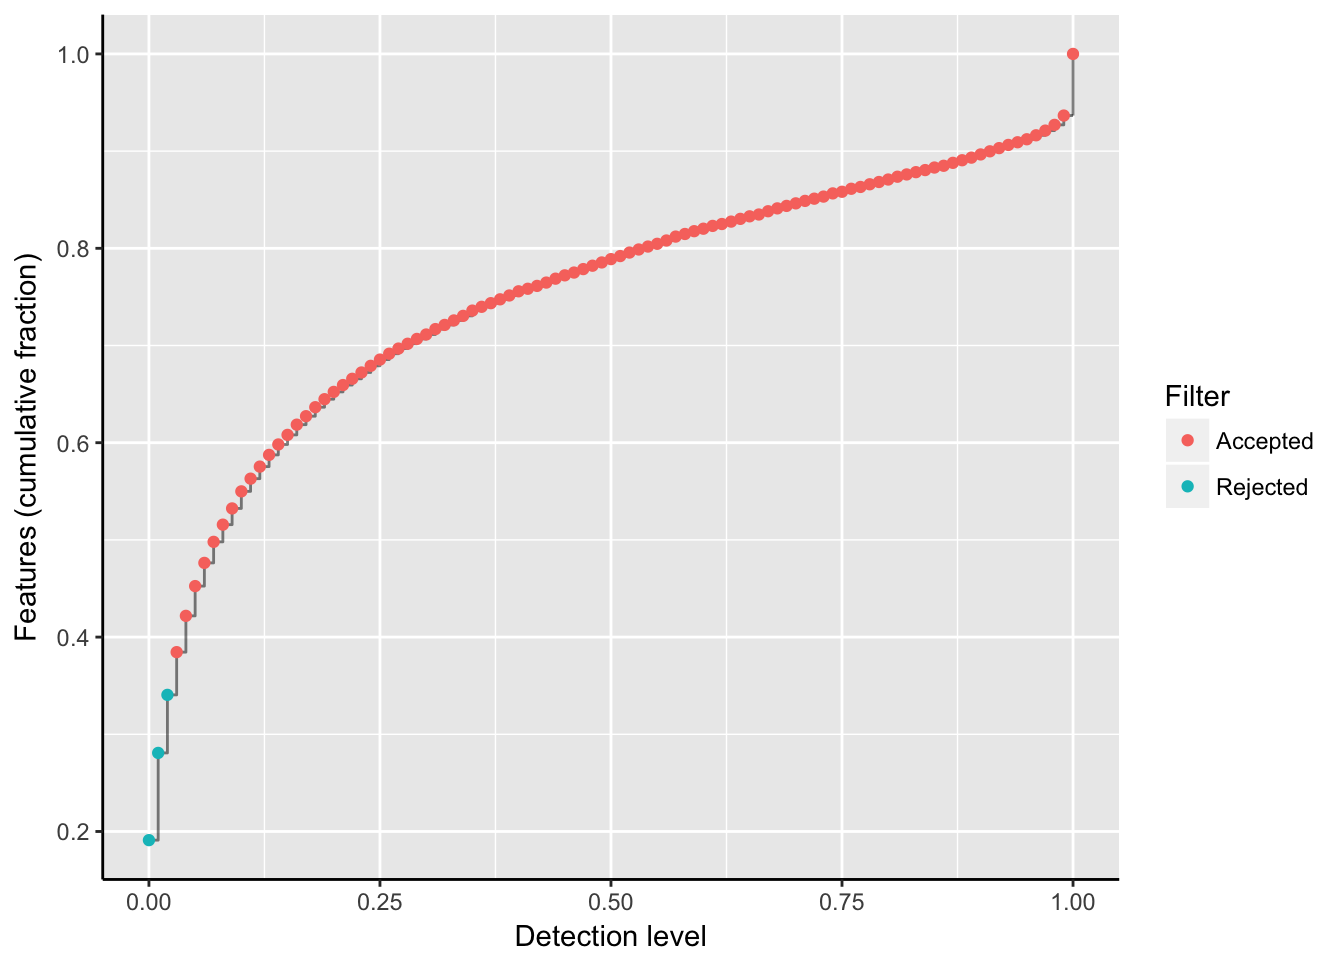
\includegraphics[width=0.7\linewidth]{CellTrails-handbook_files/figure-latex/unnamed-chunk-6-1}

\begin{Shaded}
\begin{Highlighting}[]
\NormalTok{tfeat[}\DecValTok{1}\OperatorTok{:}\DecValTok{5}\NormalTok{]}
\end{Highlighting}
\end{Shaded}

\begin{verbatim}
## [1] "feature_84" "feature_88" "feature_92" "feature_94" "feature_96"
\end{verbatim}

\begin{Shaded}
\begin{Highlighting}[]
\CommentTok{# Setting trajectory features to the object}
\KeywordTok{trajFeatureNames}\NormalTok{(exSim) <-}\StringTok{ }\NormalTok{tfeat}
\KeywordTok{showTrajInfo}\NormalTok{(exSim)}
\end{Highlighting}
\end{Shaded}

\begin{verbatim}
## [[ CellTrails ]] 
## logcounts: 15000 features, 100 samples
## Pheno data: 
##   sampleNames: "sample_1" "sample_2" ... "sample_100" (100)
##   phenoNames: none
## Feature data: 
##   featureNames: "feature_1" "feature_2" ... "feature_15000" (15000)
##   rowData: none
## Trajectory data: 
##   trajFeatureNames: "feature_84" "feature_88" ... "feature_15000" (9839)
##   latentSpace: none
##   states: none
## Trajectories: none
##   trajSampleNames: "sample_1" "sample_2" ... "sample_100" (100)
##   trajResiduals: MSE=NA
##   landmarks: none
##   trajLayout: none
## Trail data: 
##   trailNames: none
\end{verbatim}

\section{Filter by Coefficient of
Variation}\label{filter-by-coefficient-of-variation}

This filter determines trajectory features with a narrow standard
deviation (sd) with respect to its average expression (mean). This
filter removes features with high expression and low variance, such as
housekeeping genes. The coefficient of variation is computed by CoV(x) =
sd(x)/mean(x). Features with a CoV(x) greater than a given threshold
remain labeled as trajectory feature in the
\emph{\href{http://bioconductor.org/packages/SingleCellExperiment}{SingleCellExperiment}}
object. The empirical cumulative distribution function of all samples
and the fraction of removed features is shown.

\begin{Shaded}
\begin{Highlighting}[]
\CommentTok{# Filter features with COV > 0.5}
\NormalTok{tfeat <-}\StringTok{ }\KeywordTok{filterTrajFeaturesByCOV}\NormalTok{(exSim, }\DataTypeTok{threshold=}\FloatTok{0.5}\NormalTok{)}
\end{Highlighting}
\end{Shaded}

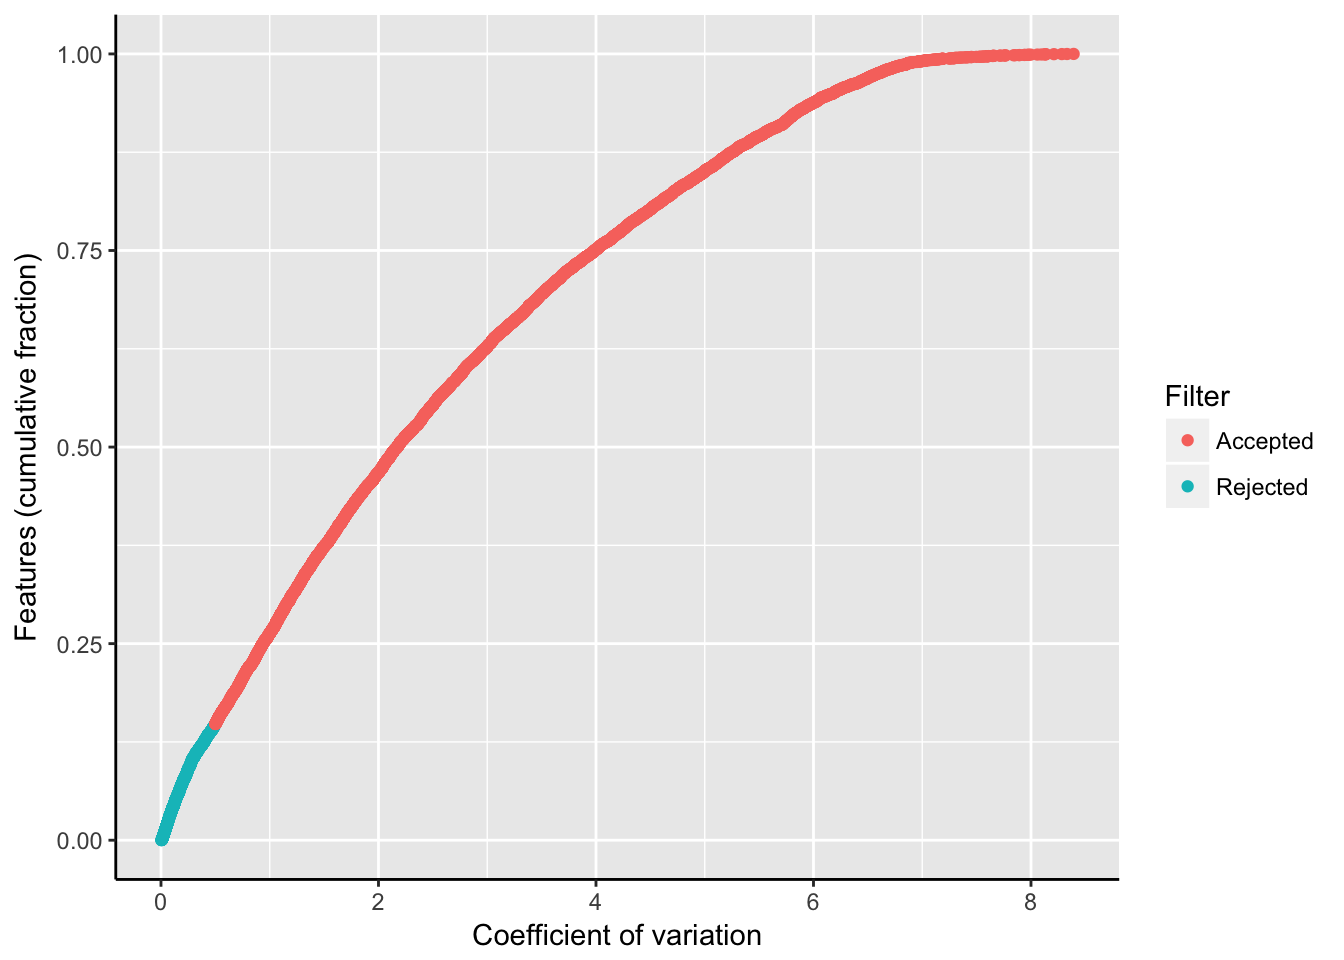
\includegraphics[width=0.7\linewidth]{CellTrails-handbook_files/figure-latex/unnamed-chunk-7-1}

\begin{Shaded}
\begin{Highlighting}[]
\CommentTok{# Setting trajectory features to the object}
\KeywordTok{trajFeatureNames}\NormalTok{(exSim) <-}\StringTok{ }\NormalTok{tfeat}
\KeywordTok{showTrajInfo}\NormalTok{(exSim)}
\end{Highlighting}
\end{Shaded}

\begin{verbatim}
## [[ CellTrails ]] 
## logcounts: 15000 features, 100 samples
## Pheno data: 
##   sampleNames: "sample_1" "sample_2" ... "sample_100" (100)
##   phenoNames: none
## Feature data: 
##   featureNames: "feature_1" "feature_2" ... "feature_15000" (15000)
##   rowData: none
## Trajectory data: 
##   trajFeatureNames: "feature_84" "feature_88" ... "feature_14998" (8386)
##   latentSpace: none
##   states: none
## Trajectories: none
##   trajSampleNames: "sample_1" "sample_2" ... "sample_100" (100)
##   trajResiduals: MSE=NA
##   landmarks: none
##   trajLayout: none
## Trail data: 
##   trailNames: none
\end{verbatim}

\section{Filter by Fano Factor}\label{filter-by-fano-factor}

This filter identifies the most variable features while considering
their average expression level. Features are placed into 20 bins based
on their mean expression. For each bin, the distribution of Fano
factors, which is a windowed version of the index of dispersion (IOD =
variance / mean), is computed and standardized (\emph{Z}-score(x) =
x/sd(x) - mean(x)/sd(x)). Highly variable features with a \emph{Z}-score
greater than a given threshold remain labeled as trajectory feature in
the
\emph{\href{http://bioconductor.org/packages/SingleCellExperiment}{SingleCellExperiment}}
object. The parameter \texttt{min\_expr} defines the minimum average
expression level of a feature to be considered for this filter (default:
0). The Fano factor and the average expression is shown for each
feature; filtered features are highlighted.

\begin{Shaded}
\begin{Highlighting}[]
\CommentTok{# Filter features with Z > 1.7}
\NormalTok{tfeat <-}\StringTok{ }\KeywordTok{filterTrajFeaturesByFF}\NormalTok{(exSim, }\DataTypeTok{threshold=}\FloatTok{1.7}\NormalTok{)}
\end{Highlighting}
\end{Shaded}

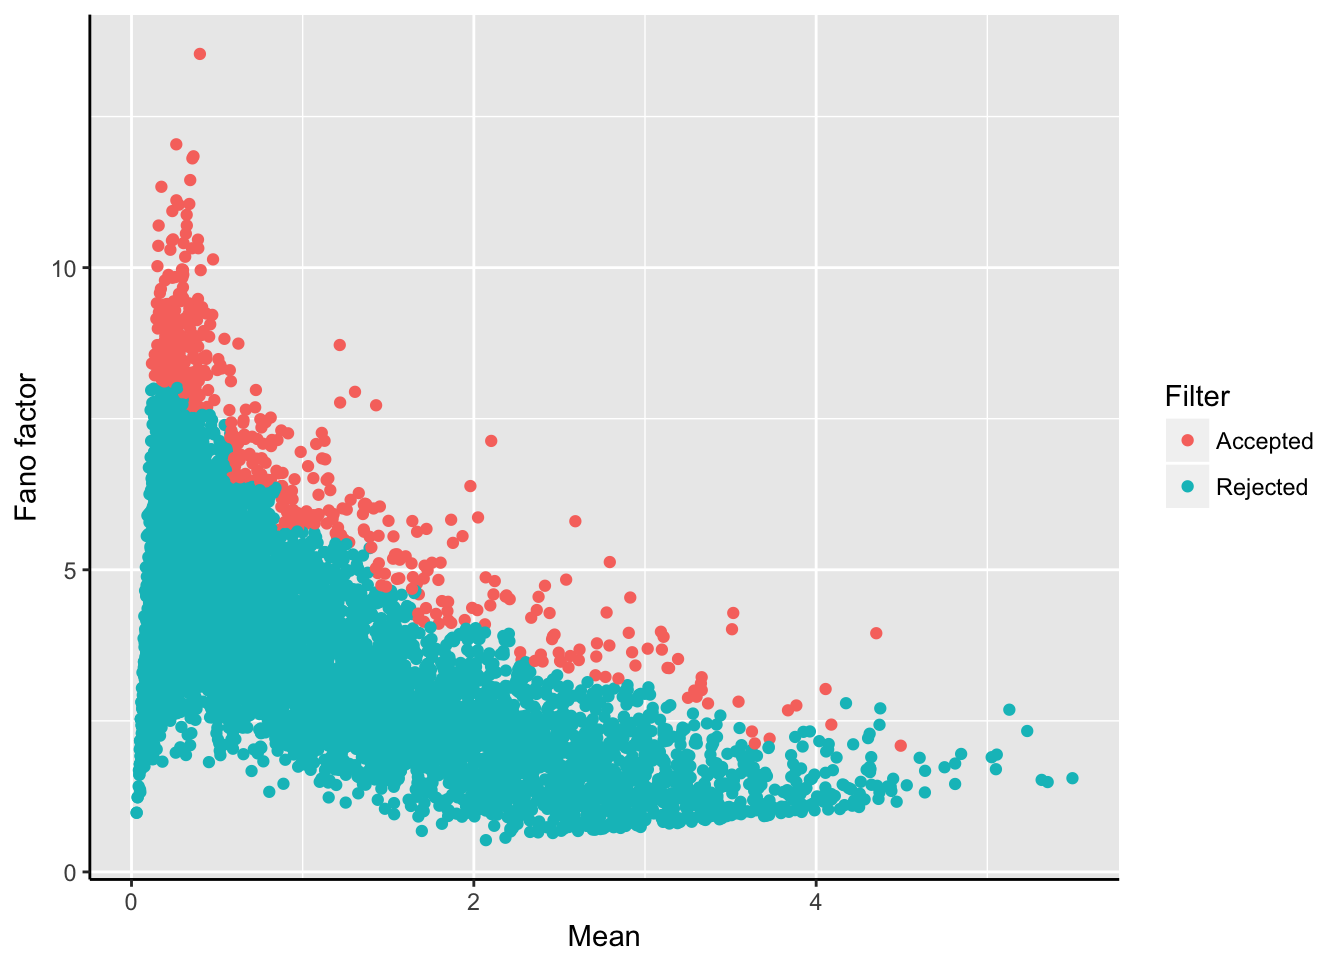
\includegraphics[width=0.7\linewidth]{CellTrails-handbook_files/figure-latex/unnamed-chunk-8-1}

\begin{Shaded}
\begin{Highlighting}[]
\CommentTok{# Setting trajectory features to the object}
\KeywordTok{trajFeatureNames}\NormalTok{(exSim) <-}\StringTok{ }\NormalTok{tfeat}
\KeywordTok{showTrajInfo}\NormalTok{(exSim)}
\end{Highlighting}
\end{Shaded}

\begin{verbatim}
## [[ CellTrails ]] 
## logcounts: 15000 features, 100 samples
## Pheno data: 
##   sampleNames: "sample_1" "sample_2" ... "sample_100" (100)
##   phenoNames: none
## Feature data: 
##   featureNames: "feature_1" "feature_2" ... "feature_15000" (15000)
##   rowData: none
## Trajectory data: 
##   trajFeatureNames: "feature_118" "feature_183" ... "feature_14998" (485)
##   latentSpace: none
##   states: none
## Trajectories: none
##   trajSampleNames: "sample_1" "sample_2" ... "sample_100" (100)
##   trajResiduals: MSE=NA
##   landmarks: none
##   trajLayout: none
## Trail data: 
##   trailNames: none
\end{verbatim}

\section{Blocking Uniformative
Substructures}\label{blocking-uniformative-substructures}

The functions \texttt{filterTrajFeaturesByCOV} and
\texttt{filterTrajFeaturesByFF} allow to define a design matrix to
account for systematic bias in the expression data (e.g., batch, gender
or cell cycle). It should list the nuisance factors that should be
blocked and their values per sample. It is suggested to construct the
design matrix with the \texttt{model.matrix} function. An example
illustrating how to create a proper design matrix is given
\protect\hyperlink{S-blockSubstructures}{here}.

\section{Using Alternative Methods}\label{using-alternative-methods}

The function \texttt{trajFeatureNames} allows to designate any set of
features as trajectory features. The only requirement is that the names
in the set match the stored feature names in the
\emph{\href{http://bioconductor.org/packages/SingleCellExperiment}{SingleCellExperiment}}
object (check with function \texttt{featureNames}). For example, one
could also use an abundance-dependent variance trend fit, as implemented
in the \emph{\href{http://bioconductor.org/packages/scran}{scran}}
package \citep{scran}, to indicate trajectory features, as shown below.
\emph{Please note} that the (Bioconductor) package
\emph{\href{http://bioconductor.org/packages/scran}{scran}} is not part
of \emph{CellTrails} and may be needed to be installed first.

\begin{Shaded}
\begin{Highlighting}[]
\NormalTok{## Not run: }
\NormalTok{##library(scran)}
\NormalTok{## End(Not run)}

\CommentTok{# Filter using scran}
\NormalTok{var_fit <-}\StringTok{ }\NormalTok{scran}\OperatorTok{::}\KeywordTok{trendVar}\NormalTok{(}\DataTypeTok{x=}\NormalTok{exSim, }\DataTypeTok{use.spikes=}\OtherTok{FALSE}\NormalTok{)}
\NormalTok{var_out <-}\StringTok{ }\NormalTok{scran}\OperatorTok{::}\KeywordTok{decomposeVar}\NormalTok{(}\DataTypeTok{x=}\NormalTok{exSim, }\DataTypeTok{fit=}\NormalTok{var_fit)}
\NormalTok{tfeat <-}\StringTok{ }\KeywordTok{featureNames}\NormalTok{(exSim)[}\KeywordTok{which}\NormalTok{(var_out}\OperatorTok{$}\NormalTok{FDR }\OperatorTok{<}\StringTok{ }\FloatTok{0.01}\NormalTok{)]}

\CommentTok{# Setting trajectory features to the object}
\KeywordTok{trajFeatureNames}\NormalTok{(exSim) <-}\StringTok{ }\NormalTok{tfeat}
\KeywordTok{showTrajInfo}\NormalTok{(exSim)}
\end{Highlighting}
\end{Shaded}

\begin{verbatim}
## [[ CellTrails ]] 
## logcounts: 15000 features, 100 samples
## Pheno data: 
##   sampleNames: "sample_1" "sample_2" ... "sample_100" (100)
##   phenoNames: none
## Feature data: 
##   featureNames: "feature_1" "feature_2" ... "feature_15000" (15000)
##   rowData: none
## Trajectory data: 
##   trajFeatureNames: "feature_118" "feature_183" ... "feature_14987" (1058)
##   latentSpace: none
##   states: none
## Trajectories: none
##   trajSampleNames: "sample_1" "sample_2" ... "sample_100" (100)
##   trajResiduals: MSE=NA
##   landmarks: none
##   trajLayout: none
## Trail data: 
##   trailNames: none
\end{verbatim}

\emph{Please note} that filters from different packages can also be
combined by subsetting the
\emph{\href{http://bioconductor.org/packages/SingleCellExperiment}{SingleCellExperiment}}
object with the trajectory features.

\begin{Shaded}
\begin{Highlighting}[]
\CommentTok{# Reset: all features are trajectory features}
\KeywordTok{trajFeatureNames}\NormalTok{(exSim) <-}\StringTok{ }\KeywordTok{featureNames}\NormalTok{(exSim)}

\CommentTok{# Use CellTrails filter}
\KeywordTok{trajFeatureNames}\NormalTok{(exSim) <-}\StringTok{ }\KeywordTok{filterTrajFeaturesByDL}\NormalTok{(exSim, }\DataTypeTok{threshold=}\DecValTok{2}\NormalTok{, }
                                                  \DataTypeTok{show_plot=}\OtherTok{FALSE}\NormalTok{)}
\KeywordTok{trajFeatureNames}\NormalTok{(exSim) <-}\StringTok{ }\KeywordTok{filterTrajFeaturesByCOV}\NormalTok{(exSim, }\DataTypeTok{threshold=}\FloatTok{0.5}\NormalTok{, }
                                                   \DataTypeTok{show_plot=}\OtherTok{FALSE}\NormalTok{)}

\NormalTok{exSim_sub <-}\StringTok{ }\NormalTok{exSim[}\KeywordTok{trajFeatureNames}\NormalTok{(exSim), ]}

\CommentTok{# Filter using scran}
\NormalTok{var_fit <-}\StringTok{ }\NormalTok{scran}\OperatorTok{::}\KeywordTok{trendVar}\NormalTok{(}\DataTypeTok{x=}\NormalTok{exSim_sub, }\DataTypeTok{use.spikes=}\OtherTok{FALSE}\NormalTok{)}
\NormalTok{var_out <-}\StringTok{ }\NormalTok{scran}\OperatorTok{::}\KeywordTok{decomposeVar}\NormalTok{(}\DataTypeTok{x=}\NormalTok{exSim_sub, }\DataTypeTok{fit=}\NormalTok{var_fit)}
\NormalTok{tfeat <-}\StringTok{ }\KeywordTok{featureNames}\NormalTok{(exSim_sub)[}\KeywordTok{which}\NormalTok{(var_out}\OperatorTok{$}\NormalTok{FDR }\OperatorTok{<}\StringTok{ }\FloatTok{0.01}\NormalTok{)]}

\CommentTok{# Setting trajectory features to the object}
\KeywordTok{trajFeatureNames}\NormalTok{(exSim) <-}\StringTok{ }\NormalTok{tfeat}
\KeywordTok{showTrajInfo}\NormalTok{(exSim)}
\end{Highlighting}
\end{Shaded}

\begin{verbatim}
## [[ CellTrails ]] 
## logcounts: 15000 features, 100 samples
## Pheno data: 
##   sampleNames: "sample_1" "sample_2" ... "sample_100" (100)
##   phenoNames: none
## Feature data: 
##   featureNames: "feature_1" "feature_2" ... "feature_15000" (15000)
##   rowData: none
## Trajectory data: 
##   trajFeatureNames: "feature_118" "feature_183" ... "feature_14987" (466)
##   latentSpace: none
##   states: none
## Trajectories: none
##   trajSampleNames: "sample_1" "sample_2" ... "sample_100" (100)
##   trajResiduals: MSE=NA
##   landmarks: none
##   trajLayout: none
## Trail data: 
##   trailNames: none
\end{verbatim}

\chapter{Manifold Learning}\label{manifold-learning}

The samples' expression profiles are shaped by many factors, such as
developmental age, tissue region of origin, cell cycle stage, as well as
extrinsic sources such as status of signaling receptors, and
environmental stressors, but also technical noise. In other words, a
single dimension, despite just containing feature expression
information, represents an underlying combination of multiple dependent
and independent, relevant and non-relevant factors, whereat each
factor's individual contribution is non-uniform. To obtain a better
resolution and to extract underlying information, \emph{CellTrails} aims
to find a meaningful low-dimensional structure - a manifold - that
represents samples mainly by their latent temporal relation.

\section{Spectral Embedding}\label{spectral-embedding}

\emph{CellTrails} aims to decipher the temporal relation between samples
by computing a novel data representation which amplifies trajectory
information in its first \emph{n} dimensions. For this purpose,
\emph{CellTrails} employs spectral graph theory. Due to their
locality-preserving character, spectral embedding techniques are
advantageous because these consider the data's manifold structure, are
insensitive to outliers and noise, are not susceptible to
short-circuiting, and emphasize naturally occurring clusters in the data
\citep{belkin2003, sussman2012}. In a nutshell, \emph{CellTrails}
assumes that two samples that have a high statistical dependency are
represented in close proximity along a trajectory. \emph{CellTrails}
captures the intrinsic data geometry as a weighted graph (nodes =
samples, edges = statistical dependencies between pairs of samples) by
means of fuzzy mutual information and uses spectral graph decomposition
to unfold the manifold revealing the hidden trajectory information.

The spectral embedding is performed using the function
\texttt{embedSamples} and results in a list with the eigenspace
representation of the original expression data.

\begin{Shaded}
\begin{Highlighting}[]
\CommentTok{# Spectral Embedding}
\NormalTok{se <-}\StringTok{ }\KeywordTok{embedSamples}\NormalTok{(exBundle)}
\end{Highlighting}
\end{Shaded}

\begin{verbatim}
## Computing adjacency matrix ...
\end{verbatim}

\begin{verbatim}
## Computing spectral embedding ...
\end{verbatim}

\begin{Shaded}
\begin{Highlighting}[]
\KeywordTok{names}\NormalTok{(se)}
\end{Highlighting}
\end{Shaded}

\begin{verbatim}
## [1] "components"  "eigenvalues"
\end{verbatim}

\emph{Please note} that this function can also be applied to any
numerical matrix of interest.

\section{Dimensionality Reduction}\label{dimensionality-reduction}

\emph{CellTrails} assumes that the expression vectors are lying on or
near a manifold with a low dimensionality that is embedded in the
higher-dimensional space. The number of dimensions can be reduced, which
lowers noise (i.e., truncates non-relevant dimensions), while the
geometry of the trajectory is emphasized.

The function \texttt{findSpectrum} helps to identify the intrisic
dimensionality of the data. It determines the most informative
dimensions based on the eigenvalues (spectrum) of the eigenspace.
Components of the latent space are ranked by their information content.
In the following example, \emph{CellTrails} identifies relevant
components by using a linear fit on the eigengaps of the first 100
eigenvalues.

\begin{Shaded}
\begin{Highlighting}[]
\CommentTok{# Identify relevant components}
\NormalTok{d <-}\StringTok{ }\KeywordTok{findSpectrum}\NormalTok{(se}\OperatorTok{$}\NormalTok{eigenvalues, }\DataTypeTok{frac=}\DecValTok{100}\NormalTok{)}
\end{Highlighting}
\end{Shaded}

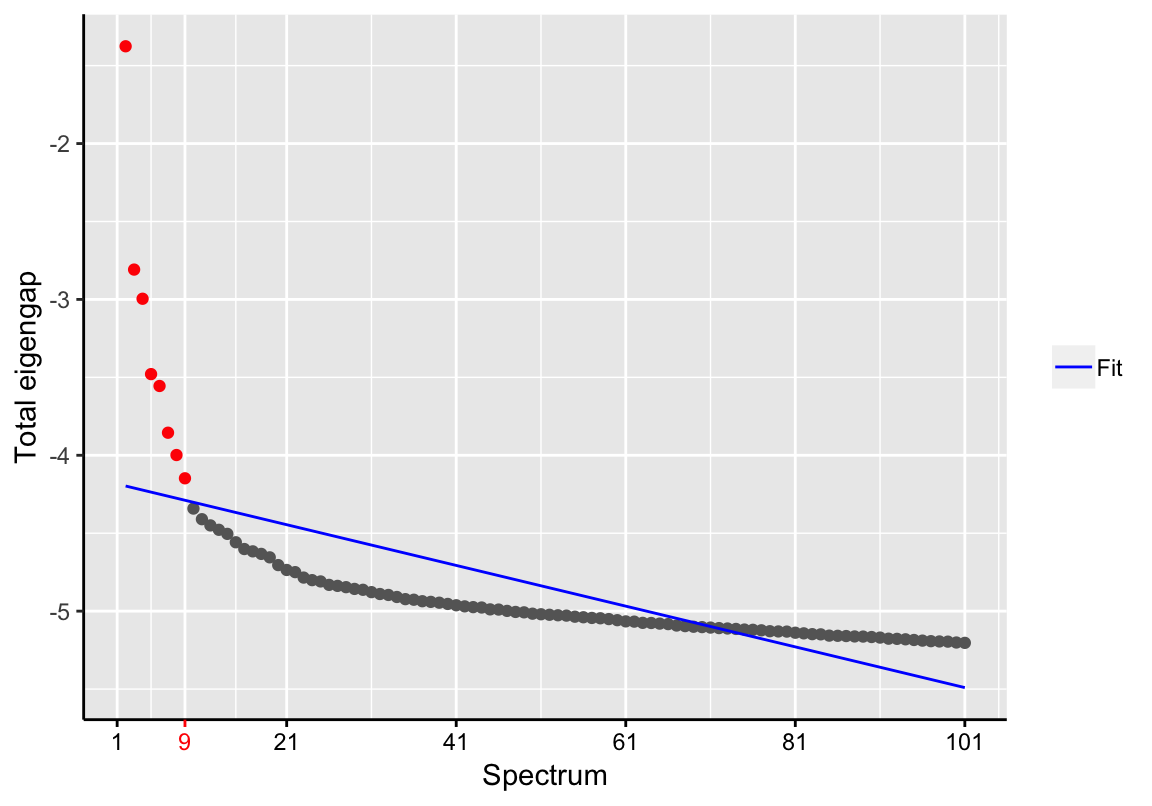
\includegraphics[width=0.7\linewidth]{CellTrails-handbook_files/figure-latex/unnamed-chunk-12-1}

\begin{Shaded}
\begin{Highlighting}[]
\NormalTok{d}
\end{Highlighting}
\end{Shaded}

\begin{verbatim}
## [1] 1 2 3 4 5 6 7 8 9
\end{verbatim}

We suggest to assess the resulting Scree plot (eigengaps versus spectrum
size) for whether the estimation of the unknown intrinsic dimensionality
was reasonable. Otherwise, we recommend to adjust the parameter
\texttt{frac} accordingly.

\emph{Please note} that considering too few components of the latent
space may result in loss of information, while selecting lower ranked
components could increase noise.

Next, we set the identified latent space to our
\emph{\href{http://bioconductor.org/packages/SingleCellExperiment}{SingleCellExperiment}}
object:

\begin{Shaded}
\begin{Highlighting}[]
\KeywordTok{latentSpace}\NormalTok{(exBundle) <-}\StringTok{ }\NormalTok{se}\OperatorTok{$}\NormalTok{components[, d]}
\end{Highlighting}
\end{Shaded}

\begin{verbatim}
## Calculating approximation of CellTrails manifold for 2D visualization...
\end{verbatim}

\begin{verbatim}
## Used tSNE perplexity: 30
\end{verbatim}

\hypertarget{S-blockSubstructures}{\section{Blocking Uninformative
Substructures}\label{S-blockSubstructures}}

Single-cell measurements are susceptible to the influence of
confounders, such as batch, gender or cell cycle effects. Blocking these
nuisance factors during manifold learning may be necessary to
significantly improve the result of downstream data analyses, such as
reconstruction of the temporal trajectory. Therefore, the function
\texttt{embedSamples} can account for confounding effects via the
parameter \texttt{design}, as will be demonstrated on the example of
single-cell RNA-Seq data of murine T helper 2 cell (T\textsubscript{h}2)
differentiation \citep{mahata2014}. In a nutshell, Buettner \emph{et
al.} \citep{buettner2015} identified cell cycle effects as major
confounder in this dataset and applied a single-cell latent variable
model (scLVM) approach to account for this factor. They unbiasedly
identified then two cell populations, namely a group of partially and a
group of fully differentiated cells. The normalized, log transformed and
filtered scRNA-Seq data can be obtained from the supplementary materials
of their article (Table S5 and S7); further, a curated list of
T\textsubscript{h}2 marker genes, the scLVM-corrected expression matrix,
and a binary cluster assignment for each cell can be downloaded.

For your convenience, the numeric expression matrix (here called
\texttt{th2}) and the list of marker genes were already organized in a
\emph{\href{http://bioconductor.org/packages/SingleCellExperiment}{SingleCellExperiment}}
container. Here, the expression matrix consists of 7,063 selected genes
(116 of which are marker genes) which have been detected in more than 3
of all 81 cells.

\begin{Shaded}
\begin{Highlighting}[]
\NormalTok{th2 <-}\StringTok{ }\KeywordTok{readRDS}\NormalTok{(}\KeywordTok{system.file}\NormalTok{(}\StringTok{"exdata"}\NormalTok{, }\StringTok{"th2.rds"}\NormalTok{, }\DataTypeTok{package=}\StringTok{"CellTrails"}\NormalTok{))}
\NormalTok{th2}
\end{Highlighting}
\end{Shaded}

\begin{verbatim}
## class: SingleCellExperiment 
## dim: 7063 81 
## metadata(0):
## assays(1): logcounts
## rownames(7063): Gnai3 Cdc45 ... ENSMUSG00000097906 X4933404O12Rik
## rowData names(2): isMarker ENSEMBL
## colnames(81): Cell 1 Cell 2 ... Cell 80 Cell 81
## colData names(0):
## reducedDimNames(0):
## spikeNames(0):
\end{verbatim}

\begin{Shaded}
\begin{Highlighting}[]
\CommentTok{# Number of markers}
\NormalTok{nMarkers <-}\StringTok{ }\KeywordTok{sum}\NormalTok{(}\KeywordTok{rowData}\NormalTok{(th2)}\OperatorTok{$}\NormalTok{isMarker)}
\NormalTok{nMarkers}
\end{Highlighting}
\end{Shaded}

\begin{verbatim}
## [1] 116
\end{verbatim}

\begin{Shaded}
\begin{Highlighting}[]
\CommentTok{# Number of total genes}
\NormalTok{nGenes <-}\StringTok{ }\KeywordTok{nrow}\NormalTok{(th2)}
\NormalTok{nGenes}
\end{Highlighting}
\end{Shaded}

\begin{verbatim}
## [1] 7063
\end{verbatim}

First, we have a quick look into the unprocessed dataset. If the latent
temporal factor is a major source of variance, two clusters, which
separate fully from partially differentiated cells, should be
detectable; if those clusters are not identifiable, the data is affected
by uniformative substructures. We assume that T\textsubscript{h}2 marker
genes should be enriched in the group of genes differentially expressed
between clusters, i.e.~the enrichment odds ratio should be
\textgreater{} 1 and the enrichment \emph{P}-value should be significant
if cells were clustered by maturity.

\begin{Shaded}
\begin{Highlighting}[]
\CommentTok{# Clustering in the original space}
\NormalTok{D <-}\StringTok{ }\KeywordTok{dist}\NormalTok{(}\KeywordTok{t}\NormalTok{(}\KeywordTok{logcounts}\NormalTok{(th2)))}
\NormalTok{dendro <-}\StringTok{ }\KeywordTok{hclust}\NormalTok{(D, }\DataTypeTok{method=}\StringTok{"ward.D2"}\NormalTok{)}
\NormalTok{cluster <-}\StringTok{ }\KeywordTok{cutree}\NormalTok{(dendro, }\DataTypeTok{k=}\DecValTok{2}\NormalTok{)}

\CommentTok{# Differential expression}
\NormalTok{pvals <-}\StringTok{ }\KeywordTok{apply}\NormalTok{(}\KeywordTok{logcounts}\NormalTok{(th2), }\DecValTok{1}\NormalTok{, }\ControlFlowTok{function}\NormalTok{(x) \{}
  \KeywordTok{wilcox.test}\NormalTok{(x[cluster }\OperatorTok{==}\StringTok{ }\DecValTok{1}\NormalTok{], }
\NormalTok{              x[cluster }\OperatorTok{==}\StringTok{ }\DecValTok{2}\NormalTok{], }
              \DataTypeTok{exact=}\OtherTok{FALSE}\NormalTok{)}\OperatorTok{$}\NormalTok{p.value\})}
\NormalTok{fdr <-}\StringTok{ }\KeywordTok{p.adjust}\NormalTok{(pvals, }\DataTypeTok{method=}\StringTok{"fdr"}\NormalTok{)}

\CommentTok{# Number of differentially expressed markers for FDR < 0.05}
\NormalTok{de <-}\StringTok{ }\KeywordTok{names}\NormalTok{(fdr[fdr }\OperatorTok{<}\StringTok{ }\FloatTok{0.05}\NormalTok{]) }\CommentTok{#differentially expressed genes}
\NormalTok{deGenes <-}\StringTok{ }\KeywordTok{length}\NormalTok{(de) }\CommentTok{#number of genes}
\NormalTok{deMarkers <-}\StringTok{ }\KeywordTok{sum}\NormalTok{(}\KeywordTok{rowData}\NormalTok{(th2[de, ])}\OperatorTok{$}\NormalTok{isMarker) }\CommentTok{#number of markers}

\CommentTok{# Enrichment statistic}
\KeywordTok{enrichment.test}\NormalTok{(deMarkers, nMarkers, deGenes, nGenes)}
\end{Highlighting}
\end{Shaded}

\begin{verbatim}
## $p.value
## [1] 0.989218
## 
## $odds.ratio
## odds ratio 
##  0.6526187 
## 
## $conf.int
## [1] 0.4687965       Inf
## attr(,"conf.level")
## [1] 0.95
## 
## $method
## [1] "Fisher's exact test for enrichment"
\end{verbatim}

Since the enrichment is not significant (with an odds ratio \textless{}
1), we argue that cells were not properly separated by maturity in the
original space.

To block the cell cycle effects, \emph{CellTrails} expects a design
matrix modeling the cell cycle stage as the explanatory factor for each
cell. As the cell-cycle stage of each cell is not known in this data
set, we need to predict cell cycle phases. In this example, we use the
classifier \texttt{cyclon} from the
\emph{\href{http://bioconductor.org/packages/scran}{scran}} package
\citep{scran}. To be able to run the algrithm properly, gene symbols
were translated to Ensembl identifiers using Bioconductors' annotation
database interface package
\emph{\href{http://bioconductor.org/packages/AnnotationDbi}{AnnotationDbi}}
\citep{R-AnnotationDbi} and the mouse annotation data package
\emph{\href{http://bioconductor.org/packages/org.Mm.eg.db}{org.Mm.eg.db}}
\citep{R-Orgmmegdb}.

\emph{Please note} that these packages are not part of \emph{CellTrails}
and may be needed to be installed first.

\begin{Shaded}
\begin{Highlighting}[]
\NormalTok{## Not run: }
\NormalTok{##library(scran)}
\NormalTok{## End(Not run)}

\CommentTok{# Run cyclone}
\NormalTok{mcm <-}\StringTok{ }\KeywordTok{readRDS}\NormalTok{(}\KeywordTok{system.file}\NormalTok{(}\StringTok{"exdata"}\NormalTok{, }\StringTok{"mouse_cycle_markers.rds"}\NormalTok{, }
                           \DataTypeTok{package=}\StringTok{"scran"}\NormalTok{))}
\KeywordTok{set.seed}\NormalTok{(}\DecValTok{1101}\NormalTok{)}
\NormalTok{cellCycle <-}\StringTok{ }\NormalTok{scran}\OperatorTok{::}\KeywordTok{cyclone}\NormalTok{(}\DataTypeTok{x=}\KeywordTok{logcounts}\NormalTok{(th2), }
                            \DataTypeTok{pairs=}\NormalTok{mcm, }
                            \DataTypeTok{gene.names=}\KeywordTok{rowData}\NormalTok{(th2)}\OperatorTok{$}\NormalTok{ENSEMBL)}

\CommentTok{# Number of predicted phases}
\KeywordTok{table}\NormalTok{(cellCycle}\OperatorTok{$}\NormalTok{phases)}
\end{Highlighting}
\end{Shaded}

\begin{verbatim}
## 
##  G1 G2M   S 
##  59  14   8
\end{verbatim}

Let's create the respective design matrix using the \texttt{cyclon}
classification scores.

\begin{Shaded}
\begin{Highlighting}[]
\CommentTok{# Design matrix}
\NormalTok{cc_design <-}\StringTok{ }\KeywordTok{model.matrix}\NormalTok{(}\OperatorTok{~}\StringTok{ }\NormalTok{cellCycle}\OperatorTok{$}\NormalTok{scores}\OperatorTok{$}\NormalTok{G1 }\OperatorTok{+}\StringTok{ }\NormalTok{cellCycle}\OperatorTok{$}\NormalTok{scores}\OperatorTok{$}\NormalTok{G2M)}
\KeywordTok{head}\NormalTok{(cc_design)}
\end{Highlighting}
\end{Shaded}

\begin{verbatim}
##   (Intercept) cellCycle$scores$G1 cellCycle$scores$G2M
## 1           1               0.108                0.701
## 2           1               1.000                0.002
## 3           1               0.971                0.009
## 4           1               1.000                0.000
## 5           1               1.000                0.000
## 6           1               0.671                0.338
\end{verbatim}

Next, we reduce the dimensionality using \emph{CellTrails}. Passing the
design matrix to \texttt{embedSamples} ensures that \emph{CellTrails}
properly regresses out the effects of the explanatory variables before
learning the manifold. Then, we cluster the cells in the derived
lower-dimensional space.

\begin{Shaded}
\begin{Highlighting}[]
\CommentTok{# Perform Dimensionality Reduction with Design Matrix}
\NormalTok{se <-}\StringTok{ }\KeywordTok{embedSamples}\NormalTok{(th2, }\DataTypeTok{design=}\NormalTok{cc_design)}
\end{Highlighting}
\end{Shaded}

\begin{verbatim}
## Warning in .embedSamples_def(x = M, design = design): Please note that
## trajectory features weren't selected. Thus, spectral embedding will be
## performed on all features, which may result in lower accuracy and longer
## computation time.
\end{verbatim}

\begin{verbatim}
## Blocking nuisance factors ...
\end{verbatim}

\begin{verbatim}
## Computing adjacency matrix ...
\end{verbatim}

\begin{verbatim}
## Computing spectral embedding ...
\end{verbatim}

\begin{Shaded}
\begin{Highlighting}[]
\NormalTok{d <-}\StringTok{ }\KeywordTok{findSpectrum}\NormalTok{(se}\OperatorTok{$}\NormalTok{eigenvalues, }\DataTypeTok{frac=}\DecValTok{60}\NormalTok{)}
\end{Highlighting}
\end{Shaded}

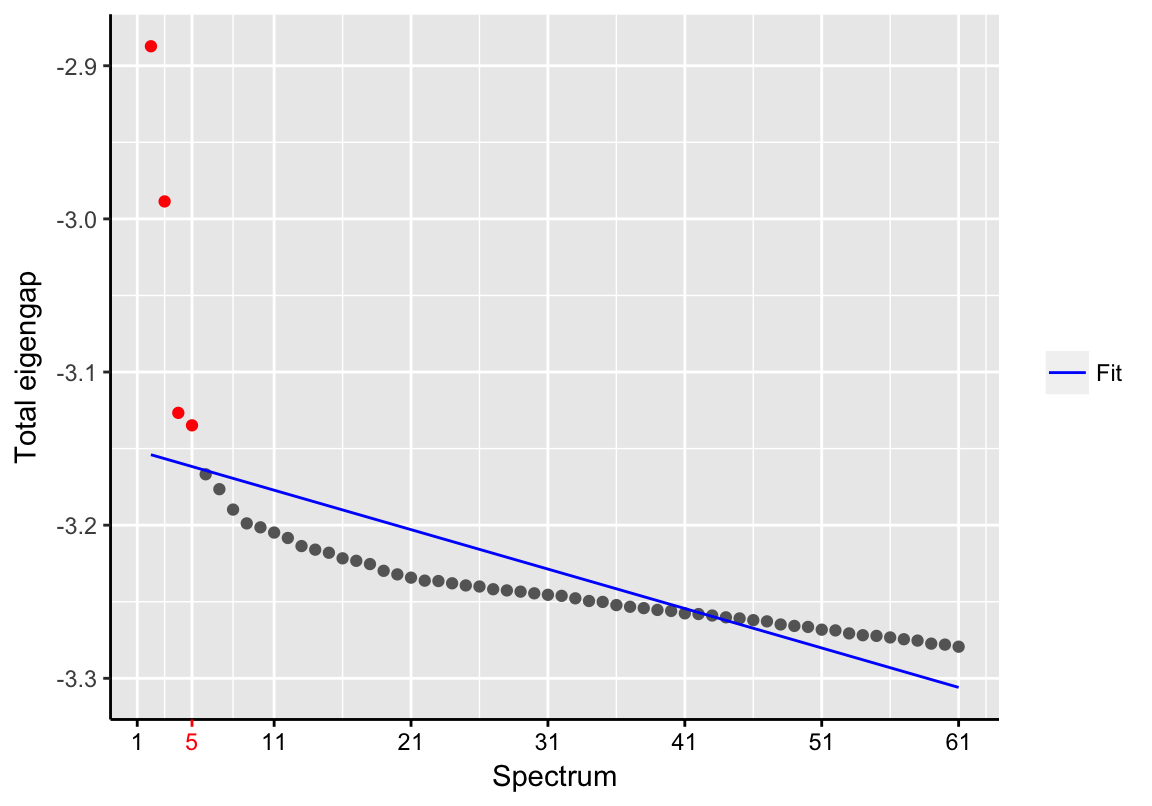
\includegraphics[width=0.7\linewidth]{CellTrails-handbook_files/figure-latex/unnamed-chunk-18-1}

\begin{Shaded}
\begin{Highlighting}[]
\KeywordTok{latentSpace}\NormalTok{(th2) <-}\StringTok{ }\NormalTok{se}\OperatorTok{$}\NormalTok{components[, d]}
\end{Highlighting}
\end{Shaded}

\begin{verbatim}
## Calculating approximation of CellTrails manifold for 2D visualization...
\end{verbatim}

\begin{verbatim}
## Used tSNE perplexity: 16
\end{verbatim}

\begin{Shaded}
\begin{Highlighting}[]
\CommentTok{# Clustering in Latent Space}
\NormalTok{D <-}\StringTok{ }\KeywordTok{dist}\NormalTok{(}\KeywordTok{latentSpace}\NormalTok{(th2))}
\NormalTok{dendro <-}\StringTok{ }\KeywordTok{hclust}\NormalTok{(D, }\DataTypeTok{method=}\StringTok{"ward.D2"}\NormalTok{)}
\NormalTok{cluster <-}\StringTok{ }\KeywordTok{cutree}\NormalTok{(dendro, }\DataTypeTok{k=}\DecValTok{2}\NormalTok{)}
\end{Highlighting}
\end{Shaded}

We test the quality of clustering by quantifying the enrichment of
marker genes in the set of differentially expressed genes.

\begin{Shaded}
\begin{Highlighting}[]
\CommentTok{# Differential expression}
\NormalTok{pvals <-}\StringTok{ }\KeywordTok{apply}\NormalTok{(}\KeywordTok{logcounts}\NormalTok{(th2), }\DecValTok{1}\NormalTok{, }\ControlFlowTok{function}\NormalTok{(x) \{}
  \KeywordTok{wilcox.test}\NormalTok{(x[cluster }\OperatorTok{==}\StringTok{ }\DecValTok{1}\NormalTok{], }
\NormalTok{              x[cluster }\OperatorTok{==}\StringTok{ }\DecValTok{2}\NormalTok{], }
              \DataTypeTok{exact=}\OtherTok{FALSE}\NormalTok{)}\OperatorTok{$}\NormalTok{p.value\})}
\NormalTok{fdr <-}\StringTok{ }\KeywordTok{p.adjust}\NormalTok{(pvals, }\DataTypeTok{method=}\StringTok{"fdr"}\NormalTok{)}

\CommentTok{# Number of differentially expressed markers for FDR < 0.05}
\NormalTok{de <-}\StringTok{ }\KeywordTok{names}\NormalTok{(fdr[fdr }\OperatorTok{<}\StringTok{ }\FloatTok{0.05}\NormalTok{]) }\CommentTok{#differentially expressed genes}
\NormalTok{deGenes <-}\StringTok{ }\KeywordTok{length}\NormalTok{(de) }\CommentTok{#number of genes}
\NormalTok{deMarkers <-}\StringTok{ }\KeywordTok{sum}\NormalTok{(}\KeywordTok{rowData}\NormalTok{(th2[de, ])}\OperatorTok{$}\NormalTok{isMarker) }\CommentTok{#number of markers}

\CommentTok{# Enrichment statistic}
\KeywordTok{enrichment.test}\NormalTok{(deMarkers, nMarkers, deGenes, nGenes)}
\end{Highlighting}
\end{Shaded}

\begin{verbatim}
## $p.value
## [1] 6.144029e-07
## 
## $odds.ratio
## odds ratio 
##   5.971408 
## 
## $conf.int
## [1] 3.431202      Inf
## attr(,"conf.level")
## [1] 0.95
## 
## $method
## [1] "Fisher's exact test for enrichment"
\end{verbatim}

The marker gene enrichment is significant (\emph{P}-value \textless{}
10\textsuperscript{-6}) and the odds ratio is remarkably increased to
\textasciitilde{}6, indicating that the cells are now properly separated
by maturity. In comparison, an enrichment odds ratio of 2.4 was achieved
using the cell-cycle `corrected' data and the clustering provided in the
original scLVM study \citep{buettner2015}.

\emph{Please note} that the differential gene expression analysis using
the \emph{CellTrails} derived clusters was performed on the actual
expression matrix and not the cell-cycle `corrected' expression values.
In contrast to scLVM, \emph{CellTrails} blocks the nuisance variables
for manifold learning only and keeps the original expression values for
downstream analysis. This is due to the fact that the manipulated
expression matrix does not represent the actual transcript levels
measured in each cell, nor does it account for the uncertainty of
estimation of the blocking factor terms. By this means,
\emph{CellTrails} protects against confounding effects without
discarding information.

Besides cell cycle, technical confounders may also be relevant to be
accounted for. Those can occur, for example, if samples were processed
on different plates or if samples were pooled from multiple sequencing
runs. In this case, a design matrix with the respective explanatory
variables can be constructed and passed to \texttt{embedSamples}.

\section{Using Alternative Methods}\label{using-alternative-methods-1}

If the user prefers to use an alternative approach for dimensionality
reduction, any latent space can be set to a
\emph{\href{http://bioconductor.org/packages/SingleCellExperiment}{SingleCellExperiment}}
object. The latent space has to be a numerical matrix; rows represent
samples and columns the components of the latent space.
\emph{CellTrails} uses by default spectral embedding, but the framework
also operates well with any other spectral dimensionality reduction
method, such as PCA (e.g., available in \emph{CellTrails} via function
\texttt{pca}) and diffusion maps (e.g., available via the
\emph{\href{http://bioconductor.org/packages/destiny}{destiny}} package
\citep{destiny}; please note this package is not part of
\emph{CellTrails} and may be needed to be installed first):

\begin{Shaded}
\begin{Highlighting}[]
\CommentTok{# Make copy of example data}
\NormalTok{exAlt <-}\StringTok{ }\NormalTok{exBundle}

\CommentTok{# PCA}
\NormalTok{pca_result <-}\StringTok{ }\KeywordTok{pca}\NormalTok{(exAlt)}
\end{Highlighting}
\end{Shaded}

\begin{verbatim}
## Warning in .pca_def(M = M, do_scaling = do_scaling, design = design): 1
## feature(s) do(es) not encode valuable information (i.e., has/have constant
## expression over all samples) and was/were therefore neglected.
\end{verbatim}

\begin{verbatim}
## Performing PCA ...
\end{verbatim}

\begin{Shaded}
\begin{Highlighting}[]
\NormalTok{d <-}\StringTok{ }\KeywordTok{findSpectrum}\NormalTok{(pca_result}\OperatorTok{$}\NormalTok{eigenvalues, }\DataTypeTok{frac=}\DecValTok{100}\NormalTok{)}
\end{Highlighting}
\end{Shaded}

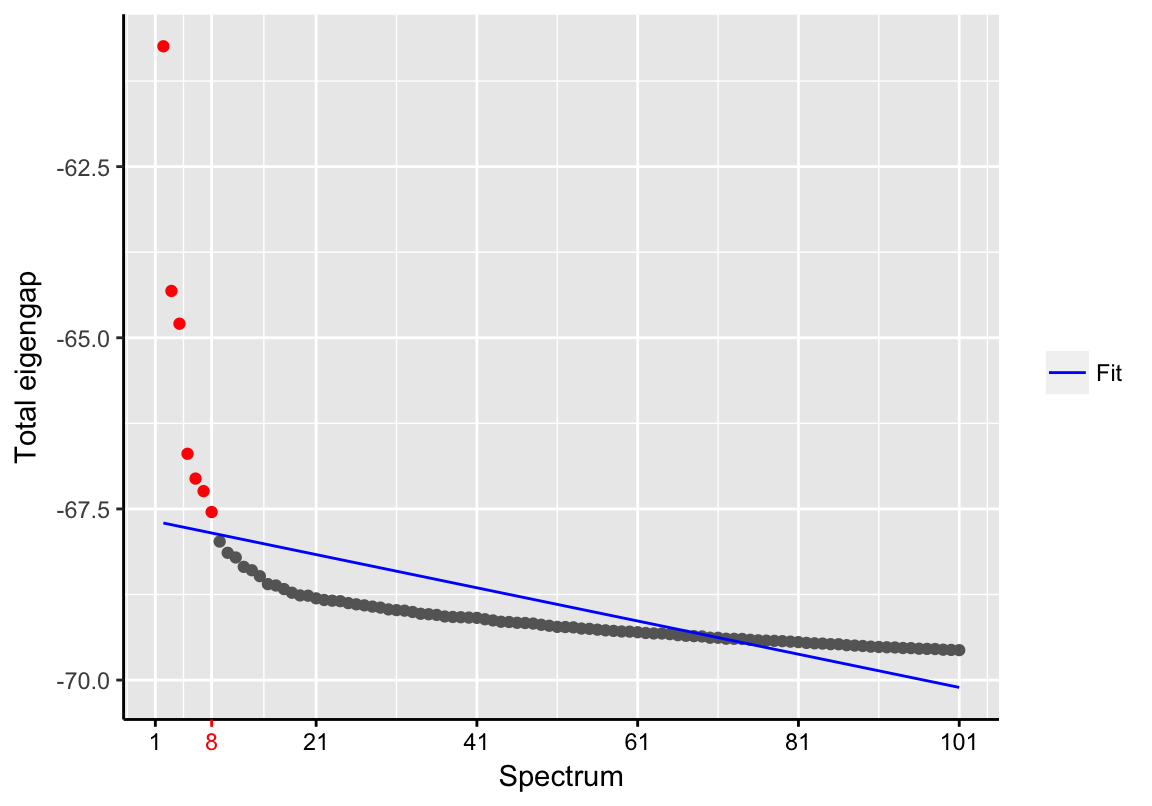
\includegraphics[width=0.7\linewidth]{CellTrails-handbook_files/figure-latex/unnamed-chunk-20-1}

\begin{Shaded}
\begin{Highlighting}[]
\KeywordTok{latentSpace}\NormalTok{(exAlt) <-}\StringTok{ }\NormalTok{pca_result}\OperatorTok{$}\NormalTok{components[, d]}
\end{Highlighting}
\end{Shaded}

\begin{verbatim}
## Calculating approximation of CellTrails manifold for 2D visualization...
\end{verbatim}

\begin{verbatim}
## Used tSNE perplexity: 30
\end{verbatim}

\begin{Shaded}
\begin{Highlighting}[]
\CommentTok{# Diffusion maps}
\NormalTok{## Not run: }
\NormalTok{##library(destiny)}
\NormalTok{## End(Not run)}

\NormalTok{lcounts <-}\StringTok{ }\KeywordTok{t}\NormalTok{(}\KeywordTok{logcounts}\NormalTok{(exAlt))}
\NormalTok{dmaps_result <-}\StringTok{ }\NormalTok{destiny}\OperatorTok{::}\KeywordTok{DiffusionMap}\NormalTok{(lcounts, }\DataTypeTok{n_eigs =} \DecValTok{101}\NormalTok{)}
\NormalTok{d <-}\StringTok{ }\KeywordTok{findSpectrum}\NormalTok{(destiny}\OperatorTok{:::}\KeywordTok{eigenvalues}\NormalTok{(dmaps_result), }\DataTypeTok{frac=}\DecValTok{100}\NormalTok{)}
\end{Highlighting}
\end{Shaded}

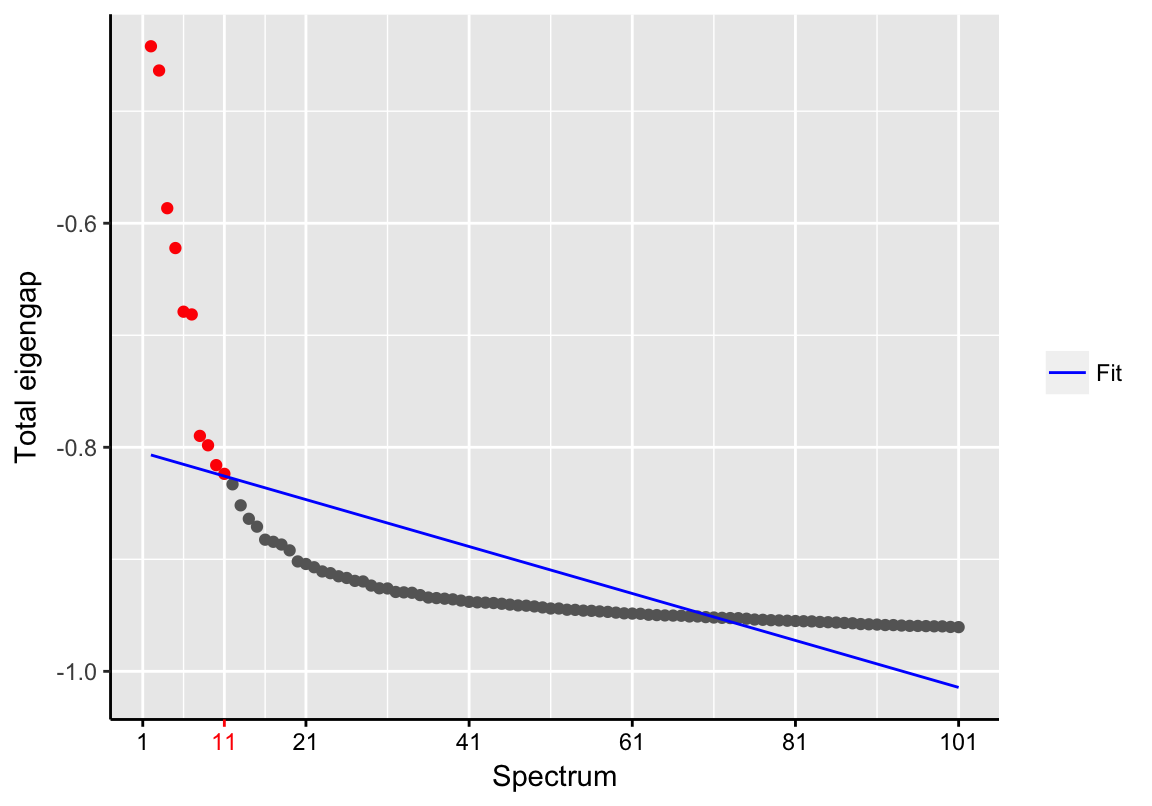
\includegraphics[width=0.7\linewidth]{CellTrails-handbook_files/figure-latex/unnamed-chunk-20-2}

\begin{Shaded}
\begin{Highlighting}[]
\KeywordTok{latentSpace}\NormalTok{(exAlt) <-}\StringTok{ }\NormalTok{destiny}\OperatorTok{:::}\KeywordTok{eigenvectors}\NormalTok{(dmaps_result)[, d]}
\end{Highlighting}
\end{Shaded}

\begin{verbatim}
## Calculating approximation of CellTrails manifold for 2D visualization...
## Used tSNE perplexity: 30
\end{verbatim}

\emph{Please note} that the function \texttt{latentSpace\textless{}-}
accepts any numerical matrix. Therefore, any latent space with an
already reduced number of dimensions can be assigned to a
\emph{CellTrailsSet} object with this function; eigenvalues are only
used to determine the intrinsic dimensionality of the data set.

\section{Visualization}\label{visualization}

\emph{CellTrails} allows us to visualize an approximation of the learned
lower-dimensional manifold in two dimensions. \emph{CellTrails'} plot
function \texttt{plotManifold} uses t-distributed stochastic neighbor
embedding (tSNE) \citep{vdmaaten2008} to illustrate the arrangement of
the samples in the latent space in a two-dimensional plot. Points denote
individual samples, the colorization indicates either a metadata label
or expression of a single feature. Empty points denote a missing label
or missing expression value (non-detects). Available phenotype lables
can be listed with the function \texttt{phenoNames}, available features
with \texttt{featureNames}, respectively.

\begin{Shaded}
\begin{Highlighting}[]
\CommentTok{# Show available phenotype labels}
\KeywordTok{phenoNames}\NormalTok{(exBundle)}
\end{Highlighting}
\end{Shaded}

\begin{verbatim}
## [1] "fm143"  "origin"
\end{verbatim}

\begin{Shaded}
\begin{Highlighting}[]
\CommentTok{# Show sample metainformation 'fm143 dye uptake'}
\KeywordTok{plotManifold}\NormalTok{(exBundle, }\DataTypeTok{color_by=}\StringTok{"phenoName"}\NormalTok{, }\DataTypeTok{name=}\StringTok{"fm143"}\NormalTok{)}
\end{Highlighting}
\end{Shaded}

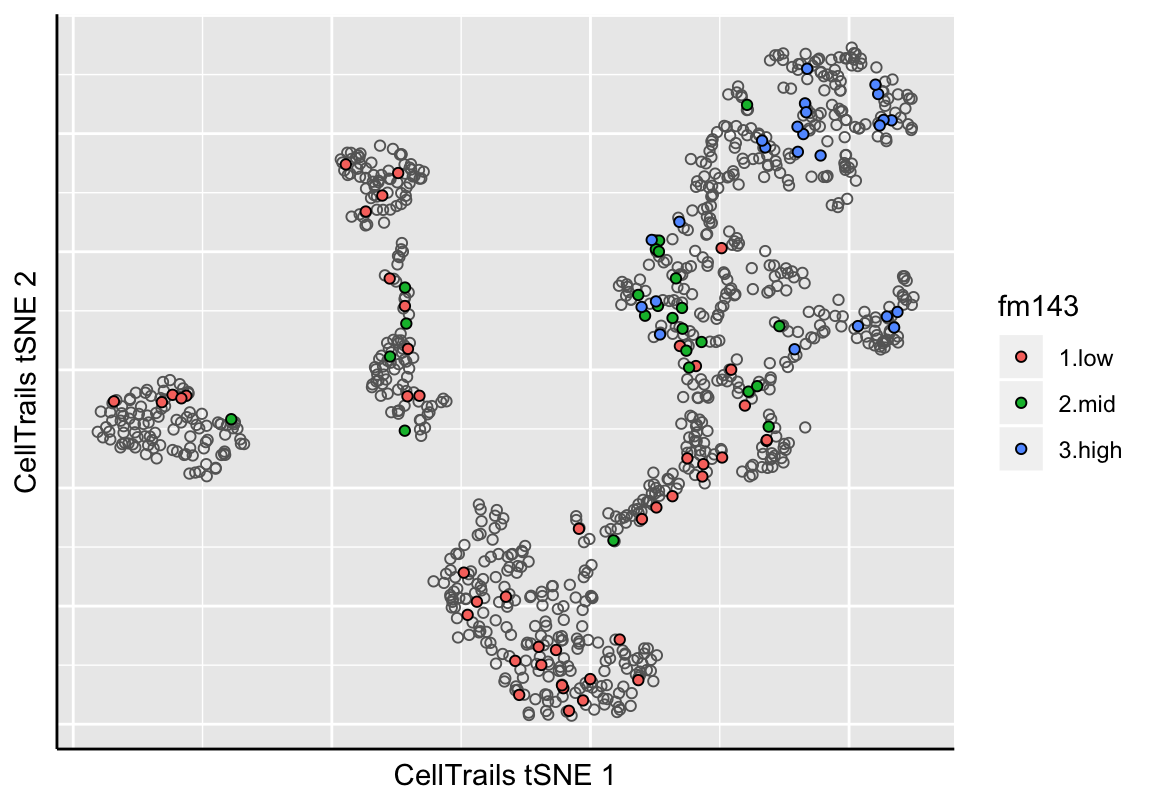
\includegraphics[width=0.7\linewidth]{CellTrails-handbook_files/figure-latex/unnamed-chunk-21-1}

The function \texttt{plotManifold} returns a \texttt{ggplot} object
\citep{ggplot2} from the
\emph{\href{https://CRAN.R-project.org/package=ggplot2}{ggplot2}}
package, which can be adapted by the user's needs and preferences (for
details, please refer to the
\emph{\href{https://CRAN.R-project.org/package=ggplot2}{ggplot2}}
manual; a plot can be exported via \texttt{ggsave}). The 2D
representation of the latent manifold is by default already stored the
the
\emph{\href{http://bioconductor.org/packages/SingleCellExperiment}{SingleCellExperiment}}
object (also accessible via \texttt{reducedDims}). However, the
\texttt{plotManifold} function provides the parameter
\texttt{recalculate}. For example, if we want to change the
\texttt{perplexity} parameter of the tSNE calculation, then we set
\texttt{recalculate=TRUE}. The new tSNE result needs to be set to the
\emph{\href{http://bioconductor.org/packages/SingleCellExperiment}{SingleCellExperiment}}
object using the \texttt{manifold2D} function, respectively.

\begin{Shaded}
\begin{Highlighting}[]
\CommentTok{# Show feature expression (e.g., gene TECTA)}
\NormalTok{gp <-}\StringTok{ }\KeywordTok{plotManifold}\NormalTok{(exBundle, }\DataTypeTok{color_by=}\StringTok{"featureName"}\NormalTok{, }\DataTypeTok{name=}\StringTok{"TECTA"}\NormalTok{, }\DataTypeTok{recalculate=}\OtherTok{TRUE}\NormalTok{)}
\end{Highlighting}
\end{Shaded}

\begin{verbatim}
## Calculating 2D approximation of CellTrails manifold...
\end{verbatim}

\begin{Shaded}
\begin{Highlighting}[]
\NormalTok{gp}
\end{Highlighting}
\end{Shaded}

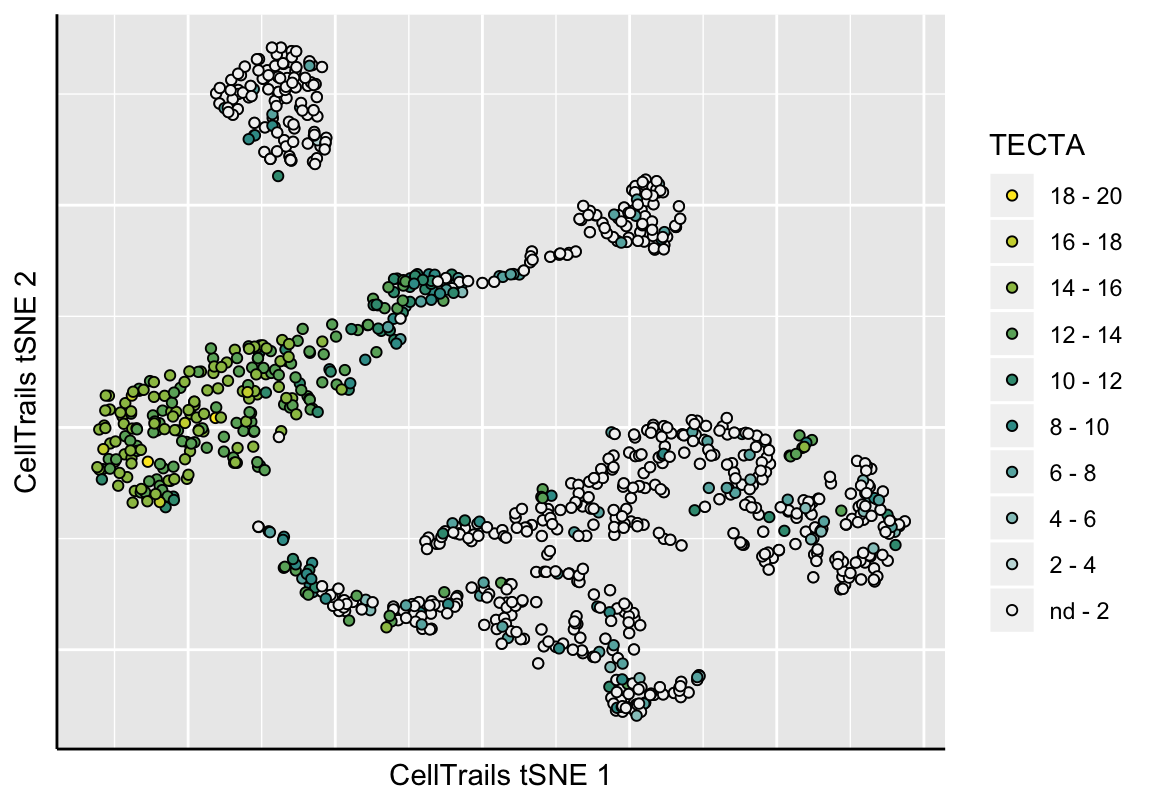
\includegraphics[width=0.7\linewidth]{CellTrails-handbook_files/figure-latex/unnamed-chunk-22-1}

\begin{Shaded}
\begin{Highlighting}[]
\CommentTok{# Store tSNE result}
\KeywordTok{manifold2D}\NormalTok{(exBundle) <-}\StringTok{ }\NormalTok{gp}

\CommentTok{# Show feature expression (e.g., genes MYO7A)}
\KeywordTok{plotManifold}\NormalTok{(exBundle, }\DataTypeTok{color_by=}\StringTok{"featureName"}\NormalTok{, }\DataTypeTok{name=}\StringTok{"MYO7A"}\NormalTok{)}
\end{Highlighting}
\end{Shaded}

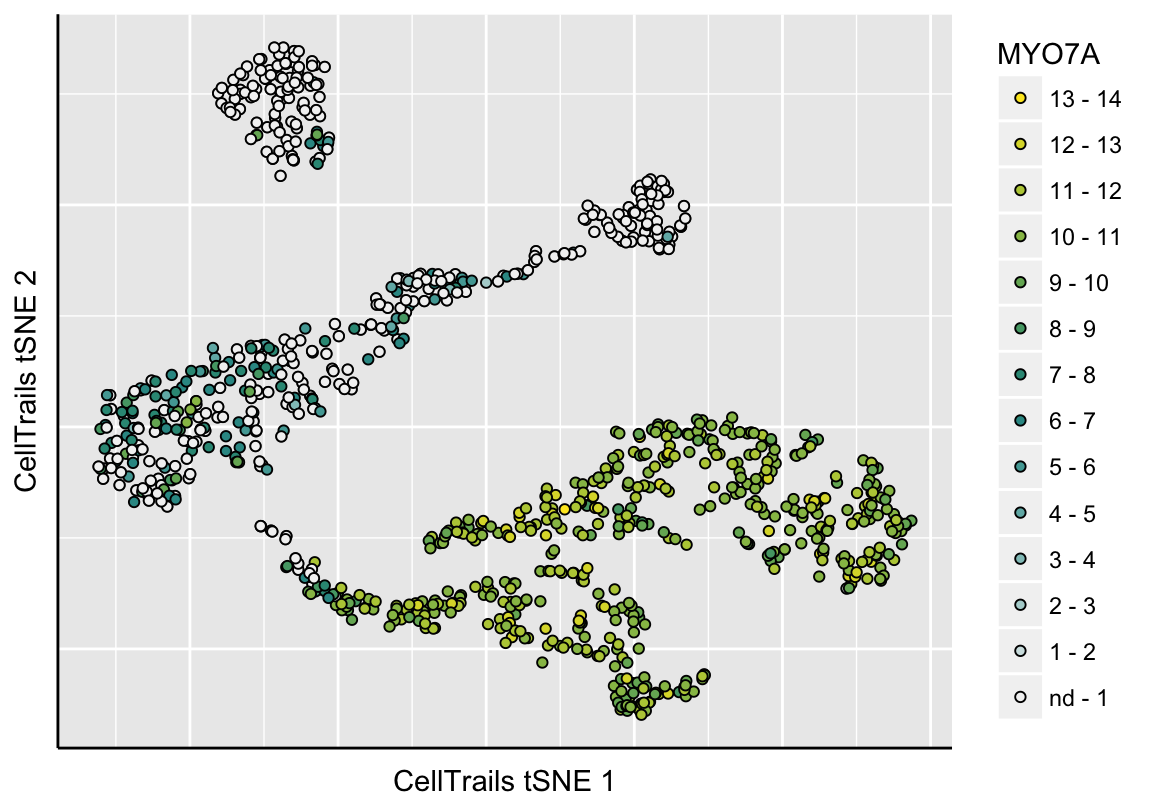
\includegraphics[width=0.7\linewidth]{CellTrails-handbook_files/figure-latex/unnamed-chunk-22-2}

\chapter{Clustering}\label{clustering}

\section{Hierarchical Spectral
Clustering}\label{hierarchical-spectral-clustering}

To identify cellular subpopulations, \emph{CellTrails} performs
hierarchical clustering via minimization of a square error criterion
\citep{ward1963} in the lower-dimensional space. To determine the number
of clusters, \emph{CellTrails} conducts an unsupervised \emph{post-hoc}
analysis. Here, it is assumed that differential expression of assayed
features determines distinct cellular stages. Hierarchical clustering in
the latent space generates a cluster dendrogram. \emph{CellTrails} makes
use of this information and identifies the maximal fragmentation of the
data space, i.e.~the lowest cutting height in the clustering dendrogram
that ensures that the resulting clusters contain at least a certain
fraction of samples. Then, processing from this height towards the root,
\emph{CellTrails} iteratively joins siblings if they do not have at
least a certain number of differentially expressed features. Statistical
significance is tested by means of a two-sample non-parametric linear
rank test accounting for censored values \citep{peto1972}. The null
hypothesis is rejected using the Benjamini-Hochberg
\citep{benjamini1995} procedure for a given significance level. The
number of clusters can impact the outcome of the trajectory
reconstruction and therefore, this step might require some parameter
tuning depending on the input data (for more information on the
parameters call \texttt{?findStates}).

\begin{Shaded}
\begin{Highlighting}[]
\NormalTok{cl <-}\StringTok{ }\KeywordTok{findStates}\NormalTok{(exBundle, }\DataTypeTok{min_size=}\FloatTok{0.01}\NormalTok{, }\DataTypeTok{min_feat=}\DecValTok{5}\NormalTok{, }\DataTypeTok{max_pval=}\FloatTok{1e-4}\NormalTok{, }\DataTypeTok{min_fc=}\DecValTok{2}\NormalTok{)}
\end{Highlighting}
\end{Shaded}

\begin{verbatim}
## Initialized 25 clusters with a minimum size of 10 samples each.
\end{verbatim}

\begin{verbatim}
## Performing post-hoc test ...
\end{verbatim}

\begin{verbatim}
## Found 11 states.
\end{verbatim}

\begin{Shaded}
\begin{Highlighting}[]
\KeywordTok{head}\NormalTok{(cl)}
\end{Highlighting}
\end{Shaded}

\begin{verbatim}
## [1] S7  S1  S4  S11 S9  S8 
## Levels: S1 S2 S3 S4 S5 S6 S7 S8 S9 S10 S11
\end{verbatim}

The clusters identified by \emph{CellTrails} are referred to as states
along the trajectory. The function \texttt{states} can be used to set
the clusters to the
\emph{\href{http://bioconductor.org/packages/SingleCellExperiment}{SingleCellExperiment}}
object.

\begin{Shaded}
\begin{Highlighting}[]
\CommentTok{# Set clusters}
\KeywordTok{states}\NormalTok{(exBundle) <-}\StringTok{ }\NormalTok{cl}
\end{Highlighting}
\end{Shaded}

State assignments are stored as sample metainformation and can be either
recieved via \texttt{colData} or \texttt{states}. Since
\texttt{CellTrails} operates on a
\emph{\href{http://bioconductor.org/packages/SingleCellExperiment}{SingleCellExperiment}}
object, its results can be easily used by other packages. For example,
visualizing a principal component analysis with
\emph{\href{http://bioconductor.org/packages/scater}{scater}}
\citep{scater}:

\begin{Shaded}
\begin{Highlighting}[]
\NormalTok{## Not run: }
\NormalTok{##library(scater)}
\NormalTok{## End(Not run)}

\CommentTok{# Plot scater PCA with CellTrails cluster information}
\NormalTok{scater}\OperatorTok{::}\KeywordTok{plotPCA}\NormalTok{(exBundle, }\DataTypeTok{colour_by=}\StringTok{"CellTrails.state"}\NormalTok{)}
\end{Highlighting}
\end{Shaded}

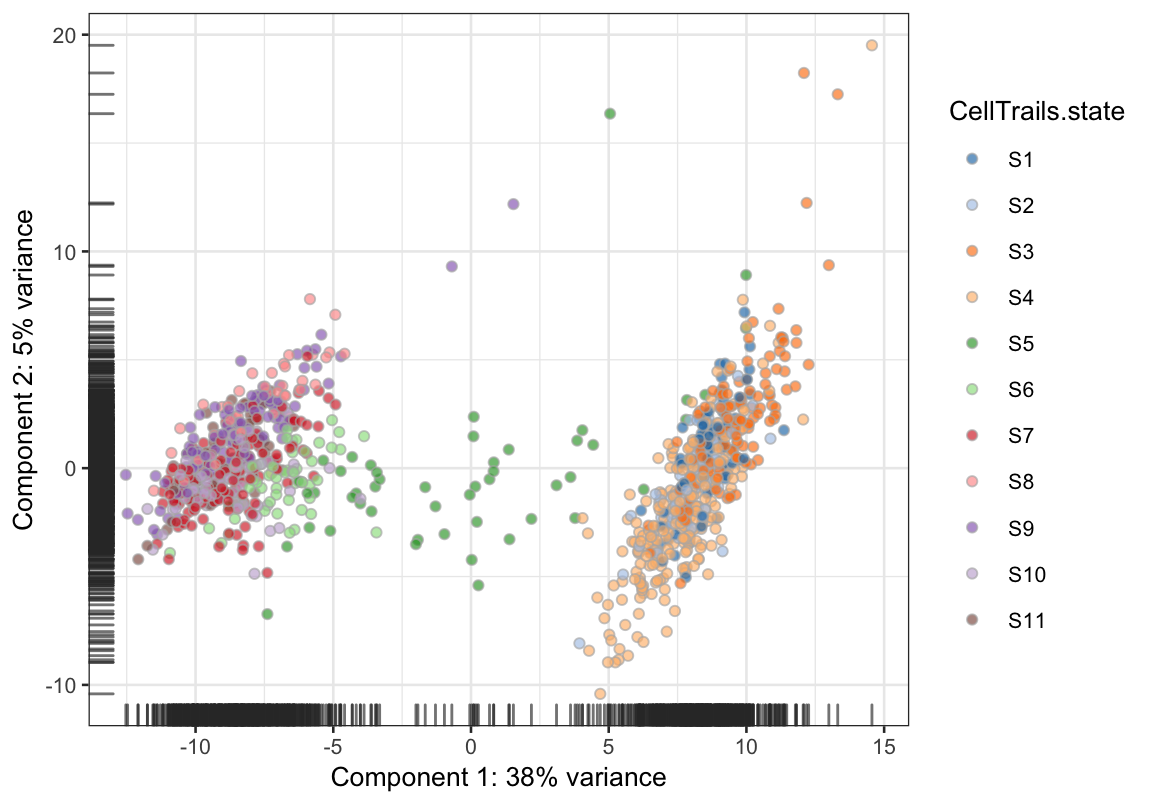
\includegraphics[width=0.7\linewidth]{CellTrails-handbook_files/figure-latex/unnamed-chunk-25-1}

Please note that the (Bioconductor) package
\emph{\href{http://bioconductor.org/packages/scater}{scater}} is not
part of \emph{CellTrails} and may be needed to be installed first.

\section{Using Alternative Methods}\label{using-alternative-methods-2}

Technically, the function \texttt{states\textless{}-} allows to set any
clustering result to a
\emph{\href{http://bioconductor.org/packages/SingleCellExperiment}{SingleCellExperiment}}
object. Any numeric, character or factor vector containing the cluster
assignments for each sample is accepted.

\section{Visualization}\label{visualization-1}

As before, we can visualize the approximated lower-dimensional manifold
and colorize each sample by its assigned state.

\begin{Shaded}
\begin{Highlighting}[]
\CommentTok{# States are now listed as phenotype}
\KeywordTok{phenoNames}\NormalTok{(exBundle)}
\end{Highlighting}
\end{Shaded}

\begin{verbatim}
## [1] "fm143"  "origin" "state"
\end{verbatim}

\begin{Shaded}
\begin{Highlighting}[]
\CommentTok{# Show manifold}
\KeywordTok{plotManifold}\NormalTok{(exBundle, }\DataTypeTok{color_by=}\StringTok{"phenoName"}\NormalTok{, }\DataTypeTok{name=}\StringTok{"state"}\NormalTok{)}
\end{Highlighting}
\end{Shaded}

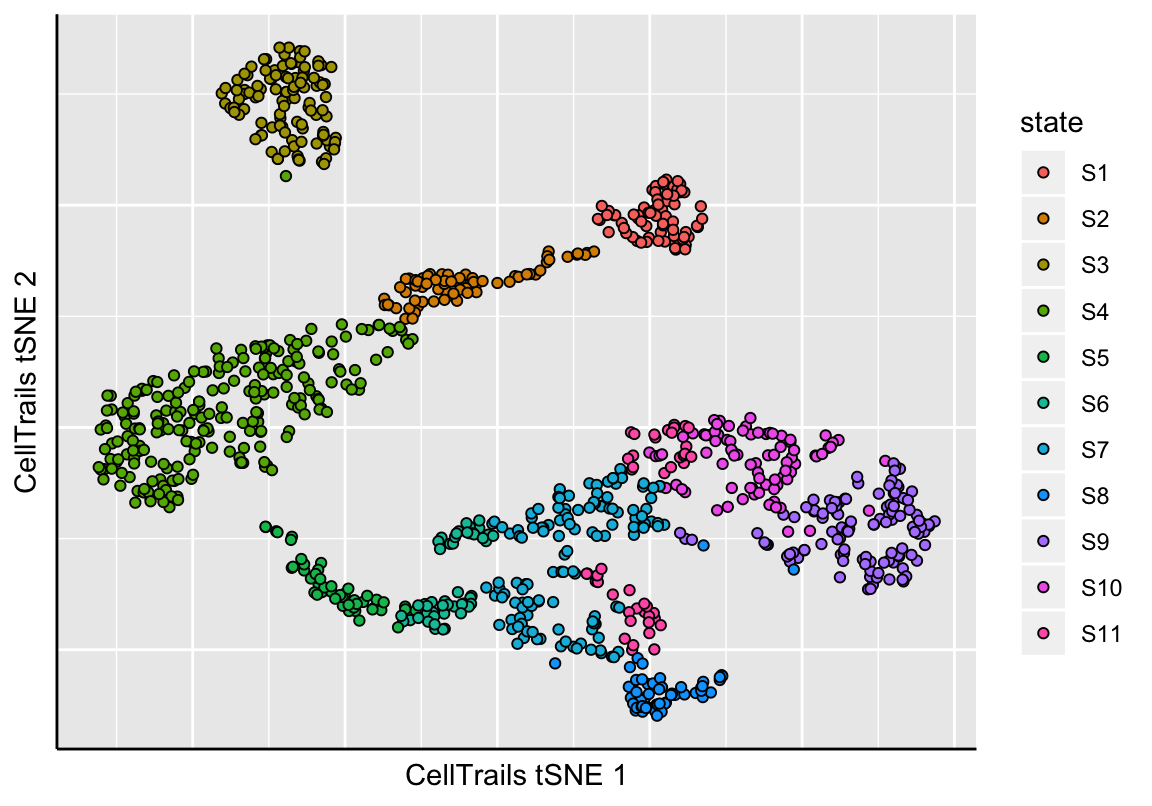
\includegraphics[width=0.7\linewidth]{CellTrails-handbook_files/figure-latex/unnamed-chunk-26-1}

The function \texttt{plotStateSize} generates a barplot showing the
absolute sizes of each state.

\begin{Shaded}
\begin{Highlighting}[]
\KeywordTok{plotStateSize}\NormalTok{(exBundle)}
\end{Highlighting}
\end{Shaded}

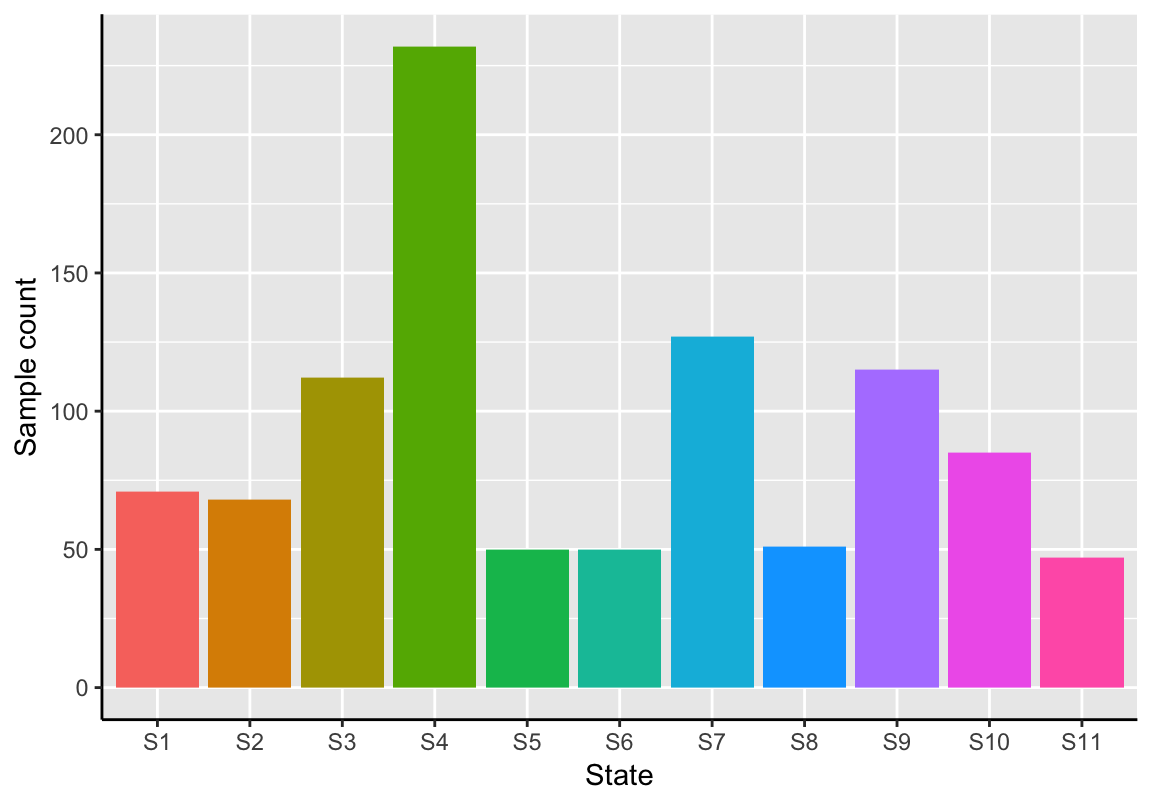
\includegraphics[width=0.7\linewidth]{CellTrails-handbook_files/figure-latex/unnamed-chunk-27-1}

Further, violin plots can be produced showing the expression
distribution of a feature per state. Each point displays the feature's
expression value in a single sample. A violine represents a vertically
mirrored density plot on each side.

\begin{Shaded}
\begin{Highlighting}[]
\KeywordTok{plotStateExpression}\NormalTok{(exBundle, }\DataTypeTok{feature_name=}\StringTok{"CALB2"}\NormalTok{)}
\end{Highlighting}
\end{Shaded}

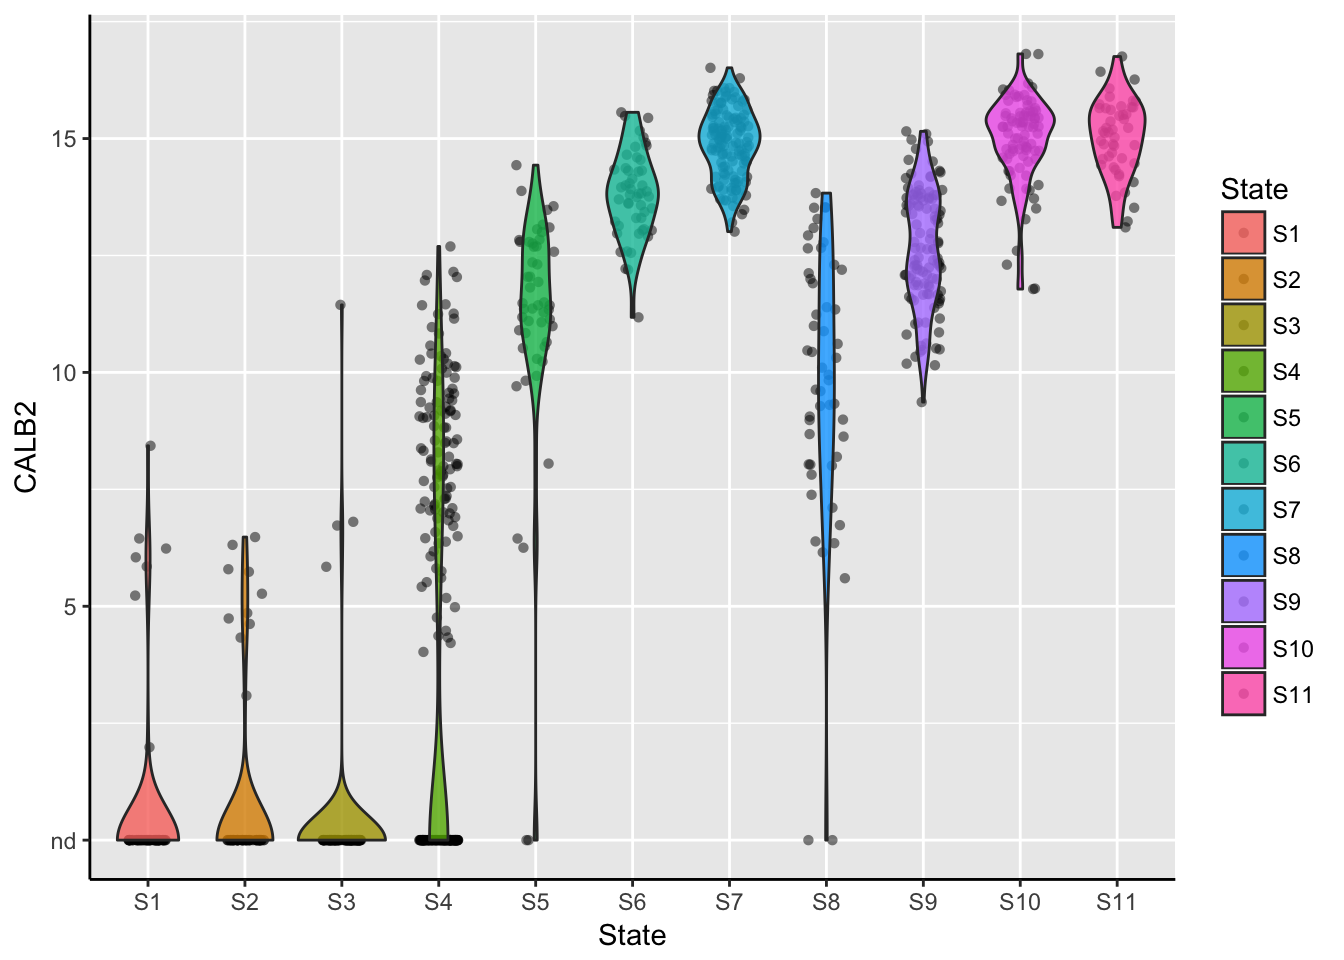
\includegraphics[width=0.7\linewidth]{CellTrails-handbook_files/figure-latex/unnamed-chunk-28-1}

\chapter{Sample Ordering}\label{sample-ordering}

\emph{CellTrails} assumes that the arrangement of samples in the
computed latent space constitutes a trajectory. \emph{CellTrails} aims
to place single samples along a maximum parsimony tree, which resembles
a branching developmental continuum. Distances between samples in the
latent space are computed using the Euclidean metric.

\section{State Trajectory Graph}\label{state-trajectory-graph}

To avoid overfitting and to facilitate the accurate identification of
bifurcations, \emph{CellTrails} simplifies the problem. Analogous to the
idea of a `broken-stick regression', \emph{CellTrails} groups the data
and performs linear fits to separate trajectory segments, which are
determined by the branching chronology of states. This leaves the
optimization problem of finding the minimum number of associations
between states that maximize the total parsimony. In theory, this
problem can be solved by any minimum spanning tree algorithm.
\emph{CellTrails} adapts this concept by assuming that adjacent states
should be located nearby and, therefore, share a relative high number of
neighboring samples.

Each state defines a submatrix of samples that is composed of a distinct
set of data vectors, i.e.~each state is a distinct set of samples
represented in the lower-dimensional space. For each state,
\emph{CellTrails} identifies the \emph{l}-nearest neighbors to each
state's data vector and takes note of their state memberships and
distances. This results in two vectors of length \emph{l} times the
state size. Subsequently, \emph{CellTrails} removes spurious neighbors
(outliers/false-positive neighbors), which are statistically too distal.
For each state \emph{CellTrails} calculates the relative frequency on
how often a state occurs in the neighborhood of a given state, which is
referred to as the interface cardinality scores.

\emph{CellTrails} implements a greedy algorithm to find the tree
maximizing the total interface cardinality score, similar to Kruskal's
minimum spanning tree algorithm \citep{kruskal1956}. The graph
construction has a relaxed requirement (number of edges \textless{}
number of nodes) compared to a tree (number of edges = number of nodes -
1), which may result in a graph having multiple tree components (=
forest) indicating potentially independent trajectories or isolated
nodes.

\emph{Please note} that the function \texttt{connectStates} can be
adjusted, such that the resulting number of components may be lower or
higher by increasing or decreasing the parameter \texttt{l},
respectively.

\begin{Shaded}
\begin{Highlighting}[]
\CommentTok{# State trajectory graph computation}
\NormalTok{exBundle <-}\StringTok{ }\KeywordTok{connectStates}\NormalTok{(exBundle, }\DataTypeTok{l=}\DecValTok{10}\NormalTok{)}
\end{Highlighting}
\end{Shaded}

\begin{verbatim}
## Calculating layout of state trajectory graph component 1...
\end{verbatim}

\begin{verbatim}
## Calculating layout of state trajectory graph component 2...
\end{verbatim}

In our example dataset, we identified two components, as indicated by
the \emph{Trajectories} entity of the \texttt{showTrajInfo} function:
component 1 is a tree with 10 states connected by 9 edges, and component
2 is an isolated state (one state, zero edges).

\begin{Shaded}
\begin{Highlighting}[]
\CommentTok{# Show trajectory information}
\KeywordTok{showTrajInfo}\NormalTok{(exBundle)}
\end{Highlighting}
\end{Shaded}

\begin{verbatim}
## [[ CellTrails ]] 
## logcounts: 183 features, 1008 samples
## Pheno data: 
##   sampleNames: "Cell-1-1" "Cell-1-2" ... "Cell-11-82" (1008)
##   phenoNames: "fm143" "origin" "state" (3)
## Feature data: 
##   featureNames: "ABCA5" "ARF1" ... "USH2A" (183)
##   rowData: none
## Trajectory data: 
##   trajFeatureNames: "ABCA5" "ARF1" ... "USH2A" (183)
##   latentSpace: 1008 samples, 9 dimensions
##   states: "S1" "S2" ... "S11" (11)
## Trajectories: [Component(#Vertices,Edges)]: 1(10,9) 2(1,0)
##   trajSampleNames: "Cell-1-1" "Cell-1-2" ... "Cell-11-82" (1008)
##   trajResiduals: MSE=NA
##   landmarks: none
##   trajLayout: none
## Trail data: 
##   trailNames: none
\end{verbatim}

The function \texttt{trajComponents} provides us information about the
states contained in each component.

\begin{Shaded}
\begin{Highlighting}[]
\CommentTok{# Show trajectory information}
\KeywordTok{trajComponents}\NormalTok{(exBundle)}
\end{Highlighting}
\end{Shaded}

\begin{verbatim}
## [[1]]
##  [1] "S1"  "S2"  "S4"  "S5"  "S6"  "S7"  "S8"  "S9"  "S10" "S11"
## 
## [[2]]
## [1] "S3"
\end{verbatim}

Further, the inferred state trajectory graph can be visualized using
\texttt{plotStateTrajectory}. If the graph is a forest, the parameter
\texttt{component} can be used to define which tree should be shown. The
optional parameters \texttt{point\_size} and \texttt{label\_offset} are
useful to adjust the graph layout, the size of the points and the
relative position of the point labels, respectively. Let's have a look
at the FM1-43 uptake and the \emph{CALB2} expression in component 1:

\begin{Shaded}
\begin{Highlighting}[]
\CommentTok{# FM1-43 uptake}
\KeywordTok{plotStateTrajectory}\NormalTok{(exBundle, }\DataTypeTok{color_by=}\StringTok{"phenoName"}\NormalTok{, }\DataTypeTok{name=}\StringTok{"fm143"}\NormalTok{, }
                    \DataTypeTok{component=}\DecValTok{1}\NormalTok{, }\DataTypeTok{point_size=}\FloatTok{1.5}\NormalTok{, }\DataTypeTok{label_offset=}\DecValTok{4}\NormalTok{)}
\end{Highlighting}
\end{Shaded}

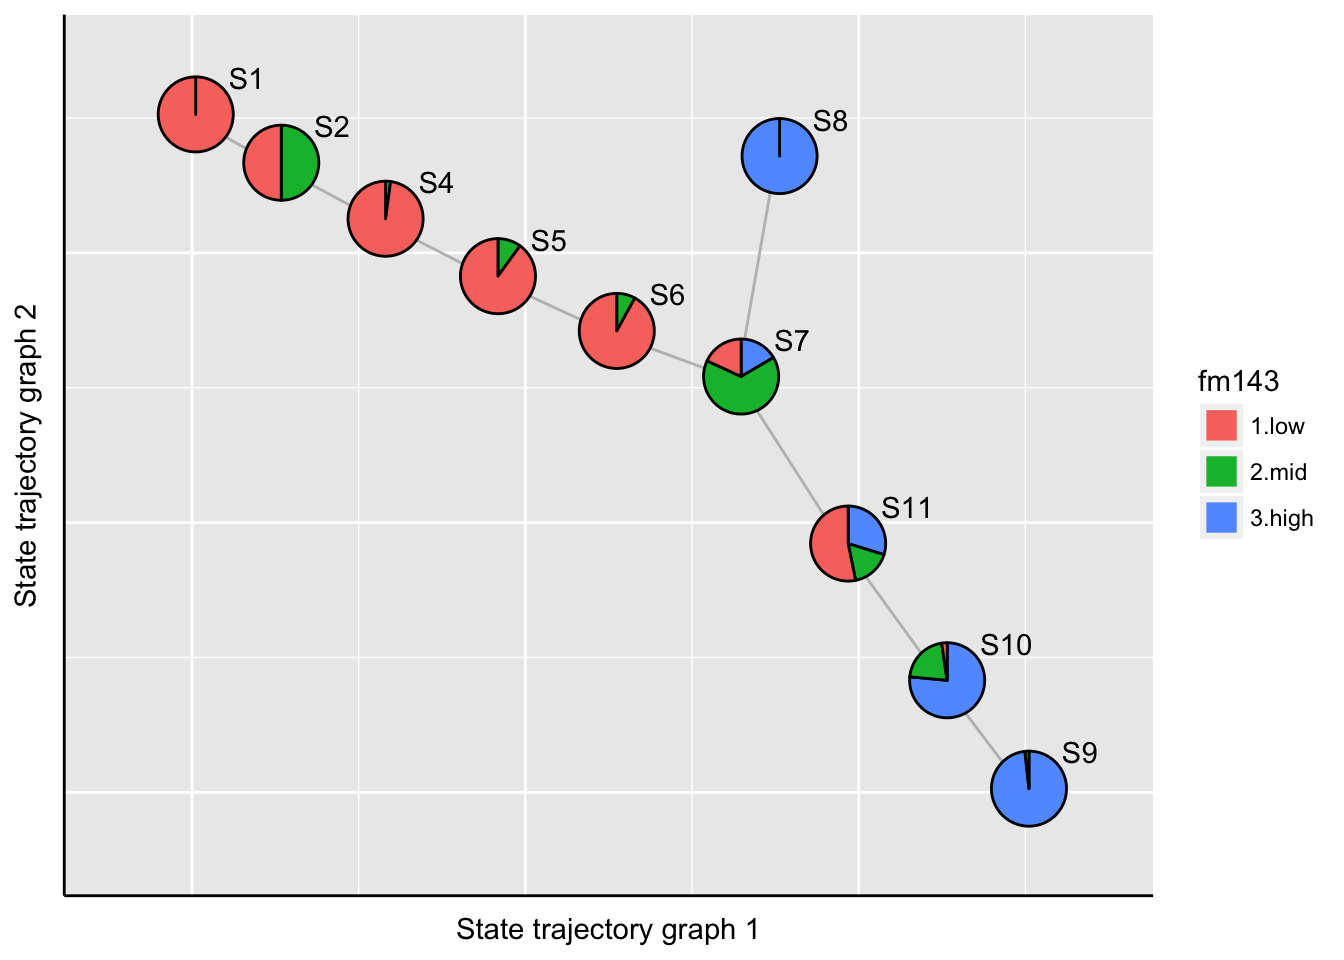
\includegraphics[width=0.7\linewidth]{CellTrails-handbook_files/figure-latex/unnamed-chunk-32-1}

The \texttt{plotStateTrajectory} function uses the Fruchterman-Reingold
graph layout algorithm \citep{fr} for visualization. If the user needs
to re-compute the layout, it can be achieved by setting the parameter
\texttt{recalculate=TRUE}. The new layout should then be stored to the
\emph{\href{http://bioconductor.org/packages/SingleCellExperiment}{SingleCellExperiment}}
object.

\begin{Shaded}
\begin{Highlighting}[]
\CommentTok{# FM1-43 uptake}
\NormalTok{gp <-}\StringTok{ }\KeywordTok{plotStateTrajectory}\NormalTok{(exBundle, }\DataTypeTok{color_by=}\StringTok{"phenoName"}\NormalTok{, }\DataTypeTok{name=}\StringTok{"fm143"}\NormalTok{, }
                          \DataTypeTok{component=}\DecValTok{1}\NormalTok{, }\DataTypeTok{point_size=}\FloatTok{1.5}\NormalTok{, }\DataTypeTok{label_offset=}\DecValTok{4}\NormalTok{, }
                          \DataTypeTok{recalculate=}\OtherTok{TRUE}\NormalTok{)}
\end{Highlighting}
\end{Shaded}

\begin{verbatim}
## Calculating layout of state trajectory graph ...
\end{verbatim}

\begin{Shaded}
\begin{Highlighting}[]
\NormalTok{gp}
\end{Highlighting}
\end{Shaded}

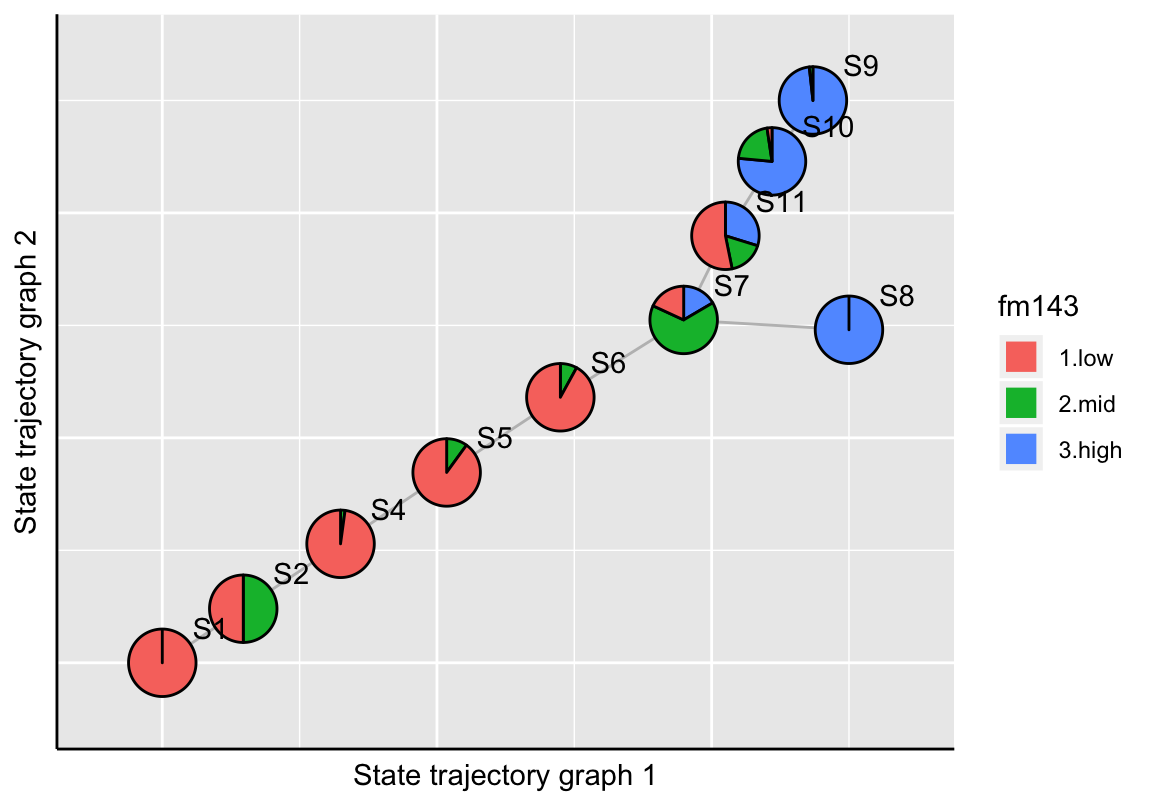
\includegraphics[width=0.7\linewidth]{CellTrails-handbook_files/figure-latex/unnamed-chunk-33-1}

\begin{Shaded}
\begin{Highlighting}[]
\CommentTok{# Store layout}
\KeywordTok{stateTrajLayout}\NormalTok{(exBundle) <-}\StringTok{ }\NormalTok{gp}

\CommentTok{# CALB2 exoression}
\KeywordTok{plotStateTrajectory}\NormalTok{(exBundle, }\DataTypeTok{color_by=}\StringTok{"featureName"}\NormalTok{, }\DataTypeTok{name=}\StringTok{"CALB2"}\NormalTok{, }
                    \DataTypeTok{component=}\DecValTok{1}\NormalTok{, }\DataTypeTok{point_size=}\DecValTok{5}\NormalTok{)}
\end{Highlighting}
\end{Shaded}

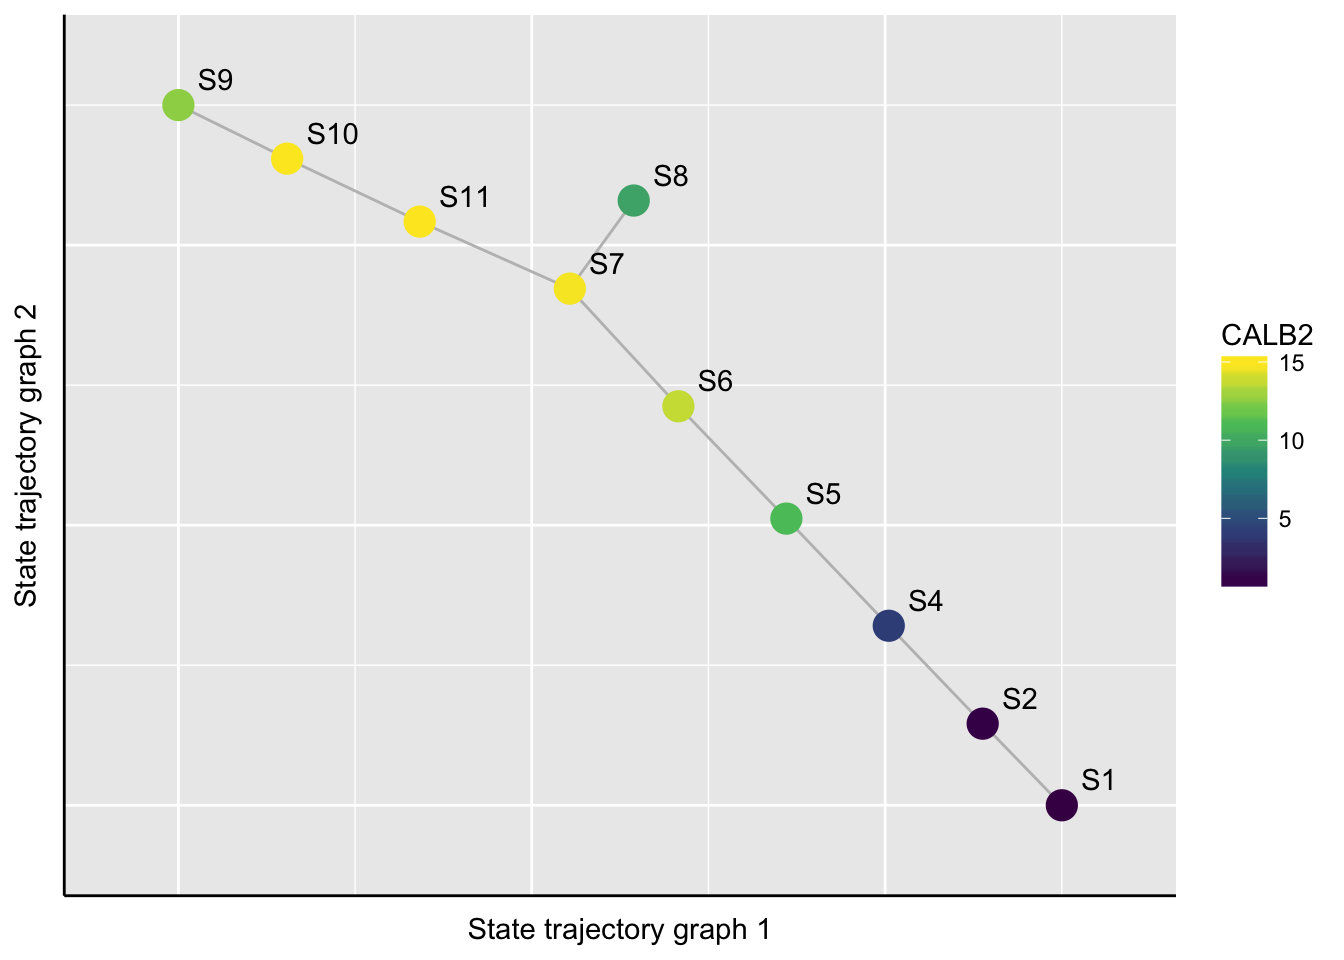
\includegraphics[width=0.7\linewidth]{CellTrails-handbook_files/figure-latex/unnamed-chunk-33-2}

\section{Aligning Samples Onto the
Trajectory}\label{aligning-samples-onto-the-trajectory}

For the sake of simplicity and performance, it makes sense to conduct
subsequent steps for each component individually. In this case, we
select the tree formed by graph component 1 with 896 samples for our
example data analysis.

\begin{Shaded}
\begin{Highlighting}[]
\CommentTok{# Select trajectory}
\NormalTok{exBundle <-}\StringTok{ }\KeywordTok{selectTrajectory}\NormalTok{(exBundle, }\DataTypeTok{component=}\DecValTok{1}\NormalTok{)}
\end{Highlighting}
\end{Shaded}

The function \texttt{trajSampleNames} returns the names of the 896
samples which were selected for trajectory reconstruction. If further
details or analyses are of interest for this set of samples exclusively,
the
\emph{\href{http://bioconductor.org/packages/SingleCellExperiment}{SingleCellExperiment}}
object can be subset.

\begin{Shaded}
\begin{Highlighting}[]
\CommentTok{# Subset SingleCellExperiment object by}
\CommentTok{# trajectory sample names}
\NormalTok{exBundle_subset <-}\StringTok{ }\NormalTok{exBundle[, }\KeywordTok{trajSampleNames}\NormalTok{(exBundle)]}

\CommentTok{# Plot state sizes}
\KeywordTok{plotStateSize}\NormalTok{(exBundle_subset)}
\end{Highlighting}
\end{Shaded}

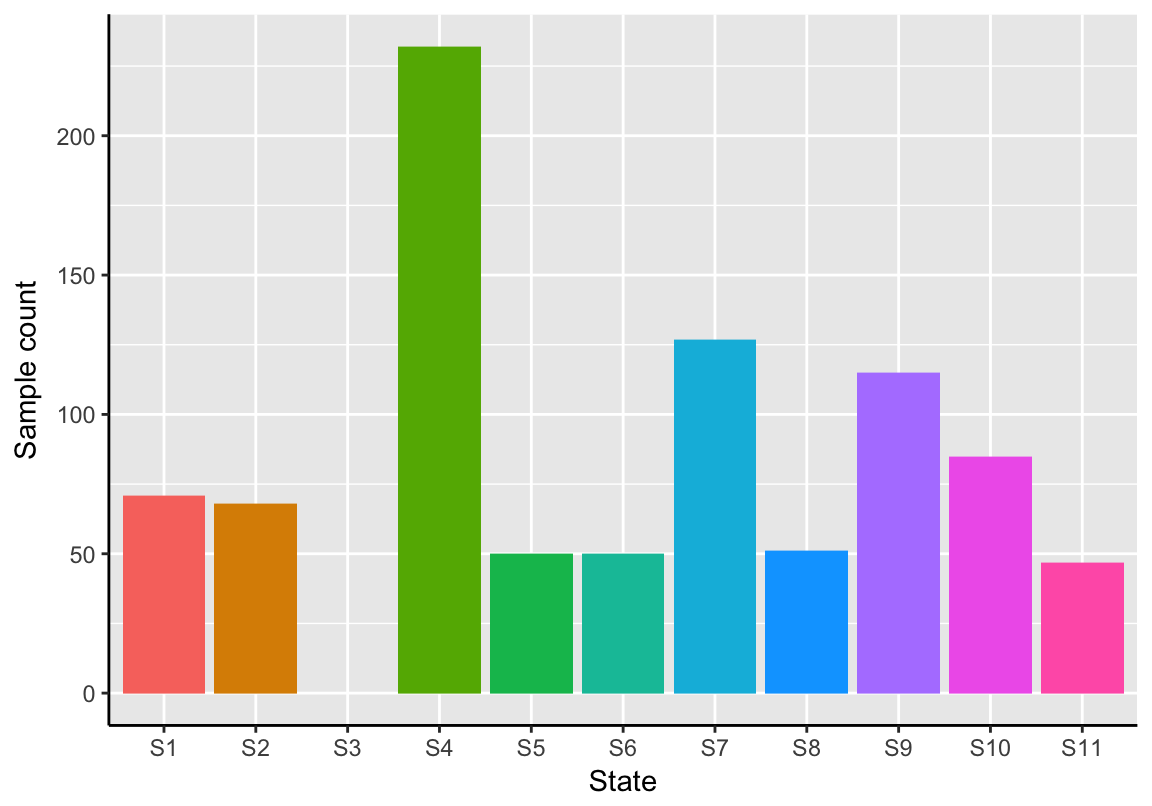
\includegraphics[width=0.7\linewidth]{CellTrails-handbook_files/figure-latex/unnamed-chunk-35-1}

As expected, the isolated state S3 (trajectory graph component 2) is not
contained in this subset.

The selected graph component defines the trajectory backbone. The
function \texttt{fitTrajectory} embeds the trajectory structure in the
latent space by computing straight lines passing through the
mediancentres \citep{bedall1979} of adjacent states. Then, a fitting
function is learned. Each sample is projected to its most proximal
straight line passing through the mediancentre of its assigned state.
Here, whenever possible, orthogonal projections onto line segments
between two mediancentres are preferred to line segments which are only
incident to a single median centre. Fitting deviations are given by the
Euclidean distance between the sample's location and the straight line,
and are indicated by an aggregated statistic (Mean Squared Error, MSE)
shown by \texttt{showTrajInfo} and can be directly accessed via
\texttt{trajResiduals}. Finally, a weighted acyclic trajectory graph can
be constructed based on each sample's position along its straight line.
Nodes in this graph are samples; edges are constructed between
neighboring samples. Each edge is weighted by the distance between its
nodes along the straight line.

\begin{Shaded}
\begin{Highlighting}[]
\CommentTok{# Align samples onto trajectory}
\NormalTok{exBundle <-}\StringTok{ }\KeywordTok{fitTrajectory}\NormalTok{(exBundle)}
\KeywordTok{showTrajInfo}\NormalTok{(exBundle)}
\end{Highlighting}
\end{Shaded}

\begin{verbatim}
## [[ CellTrails ]] 
## logcounts: 183 features, 1008 samples
## Pheno data: 
##   sampleNames: "Cell-1-1" "Cell-1-2" ... "Cell-11-82" (1008)
##   phenoNames: "fm143" "origin" ... "landmark" (4)
## Feature data: 
##   featureNames: "ABCA5" "ARF1" ... "USH2A" (183)
##   rowData: none
## Trajectory data: 
##   trajFeatureNames: "ABCA5" "ARF1" ... "USH2A" (183)
##   latentSpace: 1008 samples, 9 dimensions
##   states: "S1" "S2" ... "S11" (11)
## Trajectories: [Component(#Vertices,Edges)]: 1(10,9)
##   trajSampleNames: "Cell-1-1" "Cell-1-2" ... "Cell-11-82" (896)
##   trajResiduals: MSE=9.9e-03
##   landmarks:  #Branches=7 #Terminals=9 #User=0
##   trajLayout: none
## Trail data: 
##   trailNames: none
\end{verbatim}

\begin{Shaded}
\begin{Highlighting}[]
\KeywordTok{trajResiduals}\NormalTok{(exBundle)[}\DecValTok{1}\OperatorTok{:}\DecValTok{5}\NormalTok{]}
\end{Highlighting}
\end{Shaded}

\begin{verbatim}
## [1] 0.008616594 0.008064917 0.004659595 0.039835749 0.017354939
\end{verbatim}

Of note, the fitting function implies potential side branches in the
trajectory graph; those could be caused due to technical variance or
encompass samples that were statistically indistinguishable from the
main trajectory given the selected features used for trajectory
reconstruction. The \texttt{plotTrajectoryFit} function shows the
trajectory backbone (longest shortest path between two samples) and the
fitting deviations of each sample indicated by the perpendicular jitter.

\begin{Shaded}
\begin{Highlighting}[]
\KeywordTok{plotTrajectoryFit}\NormalTok{(exBundle)}
\end{Highlighting}
\end{Shaded}

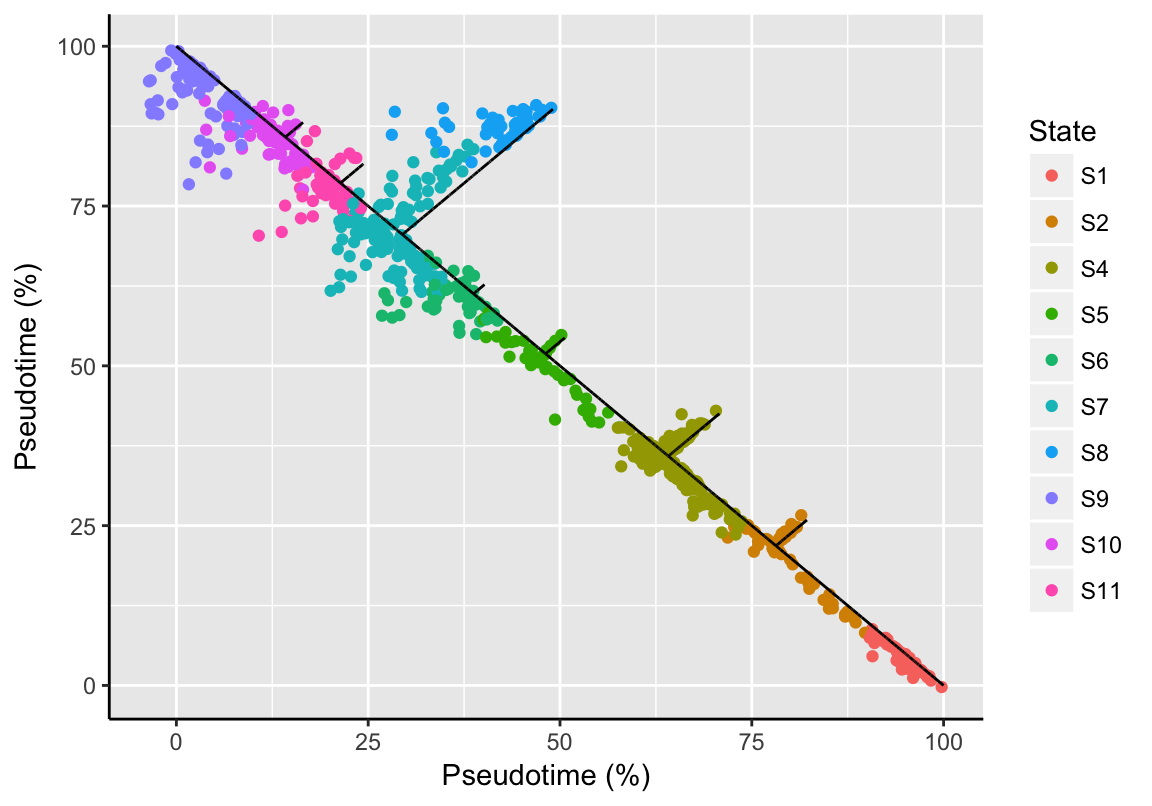
\includegraphics[width=0.7\linewidth]{CellTrails-handbook_files/figure-latex/unnamed-chunk-37-1}

\chapter{CellTrails Maps}\label{celltrails-maps}

\section{Graph Layout}\label{graph-layout}

\emph{CellTrails} portrays a computed trajectory as collection of trails
that can be found in a landscape shaped by individual expression
dynamics. To generate such a topographic trail map - the
\emph{CellTrails} map - a two-dimensional spatiotemporal ordination of
the expression matrix has to be computed. This can be done by any graph
layout algorithm using the structural information from the trajectory
graph, which is composed of nodes (=samples) and edges (=chronological
relation between samples). We found that the freely available graph
visualization software \emph{yEd}
(\url{http://www.yworks.com/products/yed}) has great capabilities to
visualize and analyze a trajectory graph. An optimal layout is planar,
i.e.~it exhibits no crossing edges or overlapping nodes.

Therefore, \emph{CellTrails} enables to export and import the trajectory
graph structure using the common \emph{graphml} file format. This file
format can be interpreted by most third-party graph analysis
applications, allowing the user to subject the trajectory graph to a
wide range of (tree) layout algorithms. In particular, the exported file
has additional ygraph attributes best suited to be used with \emph{yEd},
which is freely available for all major platforms (Windows, Mac OS, and
Linux).

\begin{Shaded}
\begin{Highlighting}[]
\KeywordTok{write.ygraphml}\NormalTok{(exBundle, }\DataTypeTok{file=}\StringTok{"yourFileName.graphml"}\NormalTok{)}
\end{Highlighting}
\end{Shaded}

Let's open the exported graphml file in \emph{yEd}:

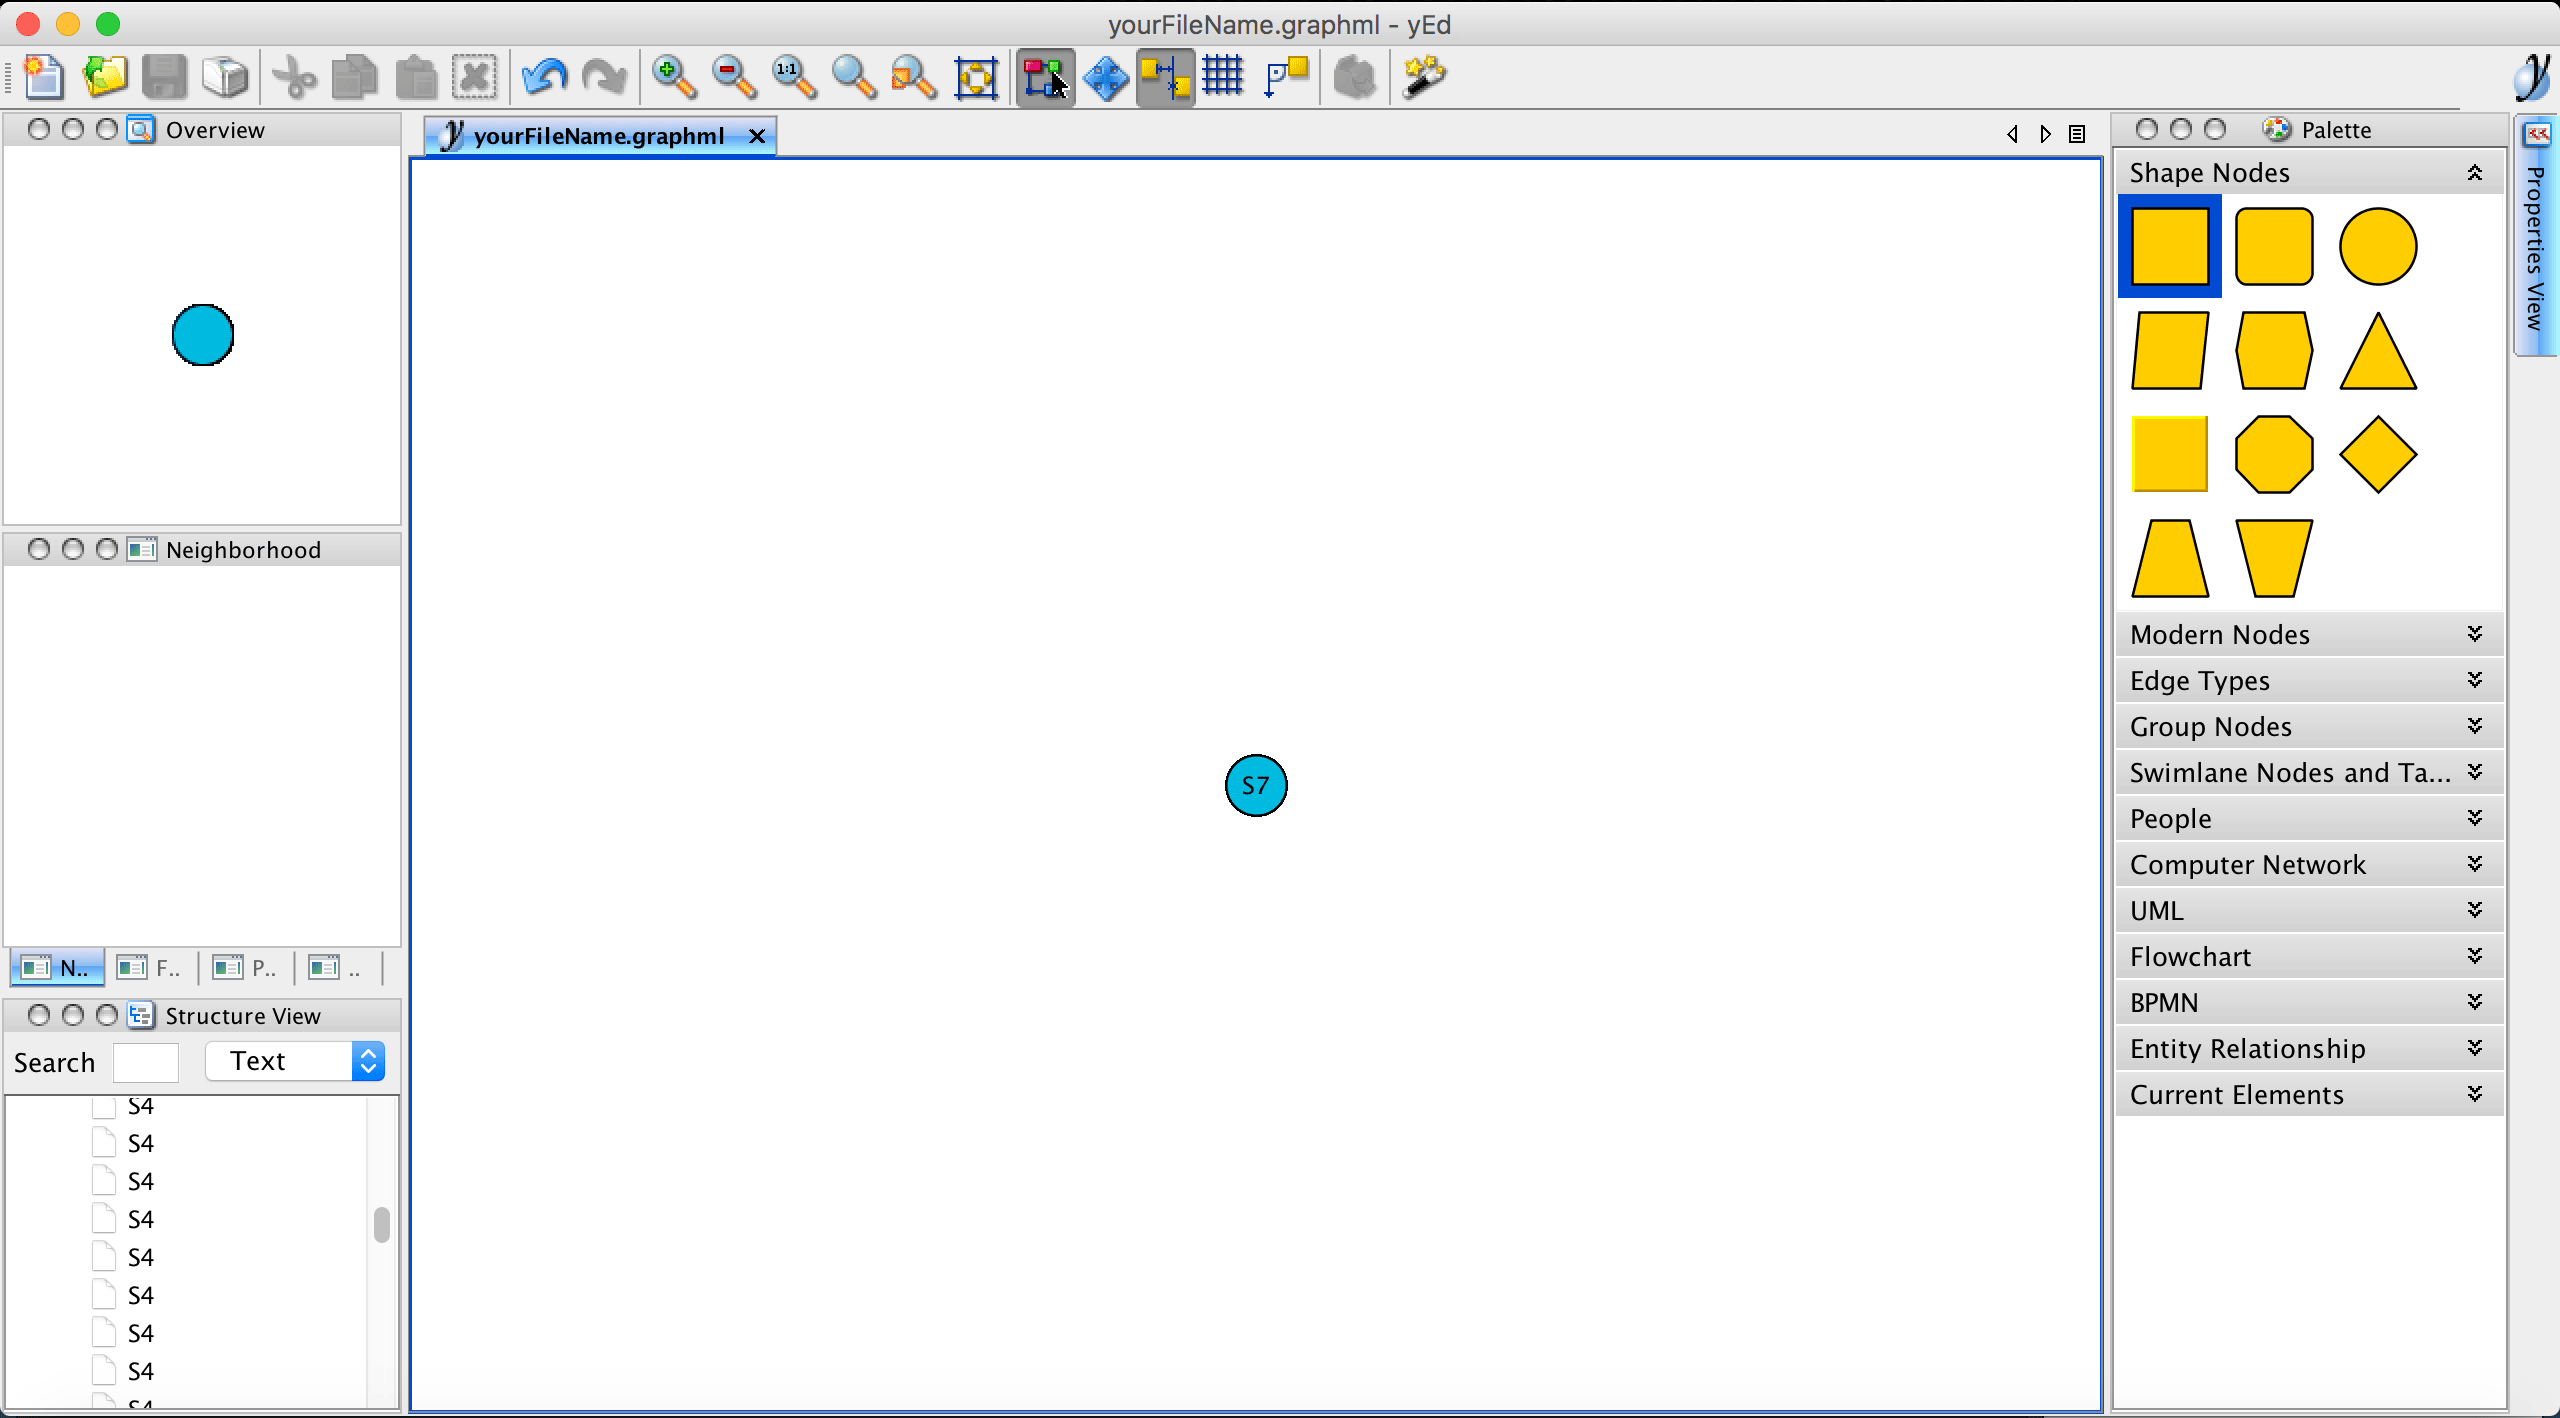
\includegraphics[width=0.7\linewidth]{img/yEd_1}

If a layout has already been defined for a
\emph{\href{http://bioconductor.org/packages/SingleCellExperiment}{SingleCellExperiment}}
object, the samples' coordinates will be listed in the exported graphml
file and will be directly interpreted by \emph{yEd}. In this example, no
layout was defined yet and therefore, all samples (nodes) are
overlapping.

\emph{Please note} that the export function \texttt{write.ygraphml}
colorizes automatically nodes by their assigned state. However, it is
possible to colorize and label nodes by any phenotype or feature
expression data stored in the
\emph{\href{http://bioconductor.org/packages/SingleCellExperiment}{SingleCellExperiment}}
object. For example, we could colorize the nodes by the recorded FM1-43
dye intensity to get an idea where the trajectory might start and end (a
high FM1-43 dye indicates mature cells) and label the nodes by their
determined state by setting the parameters
\texttt{color\_by="phenoName"}, \texttt{name="fm143"} and
\texttt{label="state"}. Nodes with a missing phenotype information are
not colorized and remain transparent.

Next, we layout the graph. Since the trajectory resembles a tree
structre, we use a tree algorithm. We found that routing the trajectory
graph in a quasi-radial style, called balloon style, works very well for
our case. The layouter can be selected via \emph{Layout} \(\rightarrow\)
\emph{Tree} \(\rightarrow\) \emph{Balloon}. The following parameter
setting was used in the original \emph{CellTrails} publication:

\includegraphics[width=0.7\linewidth]{img/yEd_2-3}

Let's run the algorithm to compute the layout:

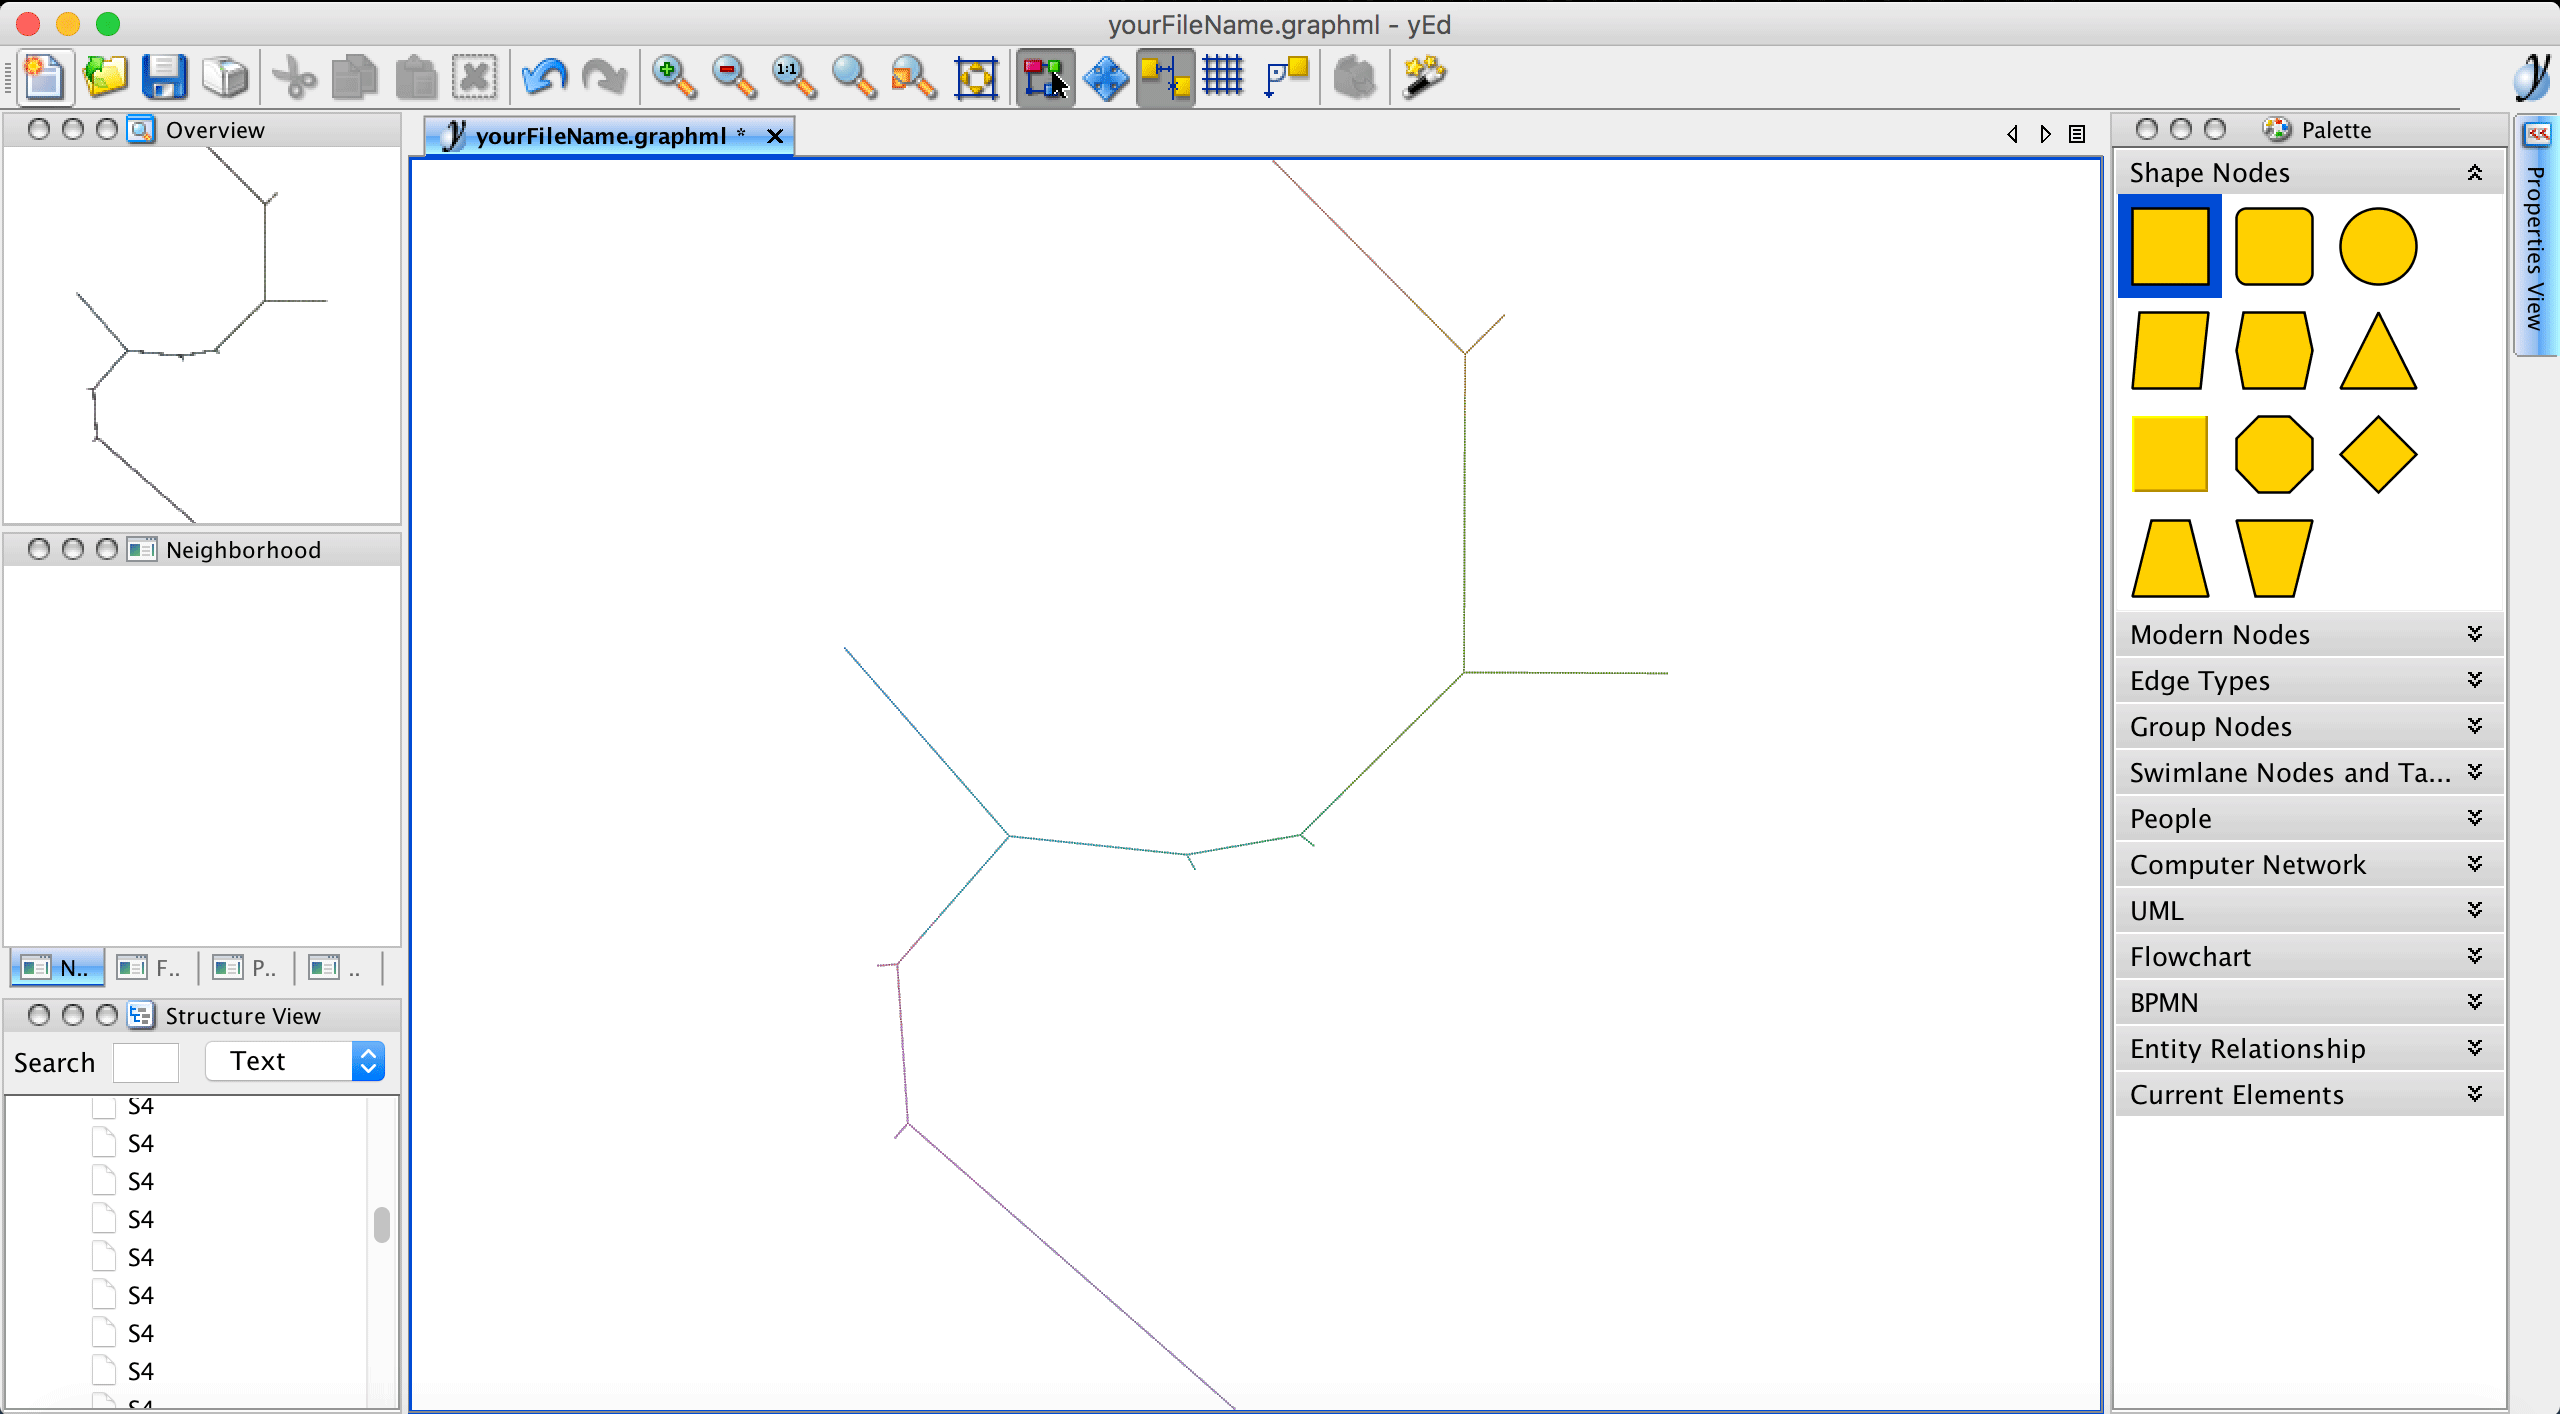
\includegraphics[width=0.7\linewidth]{img/yEd_4}

\emph{Please note} that edge crossings (i.e., two or more edges overlap)
are not useful and if they occur we suggest to re-run the layouter with
different parameters before saving the layout. Using either your mouse
or the \emph{View} \(\rightarrow\) \emph{Zoom In} option allows to have
a closer look. If we want to have the trajectory progressing from bottom
left to bottom right (based on a specific feature expression or
phenotype label), we need to transform the graph. This can be done via
\emph{Tools} \(\rightarrow\) \emph{Geometric transformations}. Here, we
select \emph{Mirror on Y axis} and \emph{Mirror on X axis}.

\includegraphics[width=0.7\linewidth]{img/yEd_5-6}

Finally, the file can be saved via \emph{File} \(\rightarrow\)
\emph{Save} and reimported to R.

\begin{Shaded}
\begin{Highlighting}[]
\NormalTok{tl <-}\StringTok{ }\KeywordTok{read.ygraphml}\NormalTok{(}\StringTok{"yourFileName.graphml"}\NormalTok{)}
\end{Highlighting}
\end{Shaded}

For illustration purposes, the computed trajectory layout for the
example dataset is available within this package.

\begin{Shaded}
\begin{Highlighting}[]
\CommentTok{# Import layout}
\NormalTok{tl <-}\StringTok{ }\KeywordTok{read.ygraphml}\NormalTok{(}\KeywordTok{system.file}\NormalTok{(}\StringTok{"exdata"}\NormalTok{, }\StringTok{"bundle.graphml"}\NormalTok{, }
                                \DataTypeTok{package=}\StringTok{"CellTrails"}\NormalTok{))}

\CommentTok{# Plot layout}
\KeywordTok{plot}\NormalTok{(tl[,}\DecValTok{1}\OperatorTok{:}\DecValTok{2}\NormalTok{], }\DataTypeTok{axes=}\OtherTok{FALSE}\NormalTok{, }\DataTypeTok{xlab=}\StringTok{""}\NormalTok{, }\DataTypeTok{ylab=}\StringTok{""}\NormalTok{, }\DataTypeTok{pch=}\DecValTok{20}\NormalTok{, }\DataTypeTok{cex=}\NormalTok{.}\DecValTok{25}\NormalTok{)}
\end{Highlighting}
\end{Shaded}

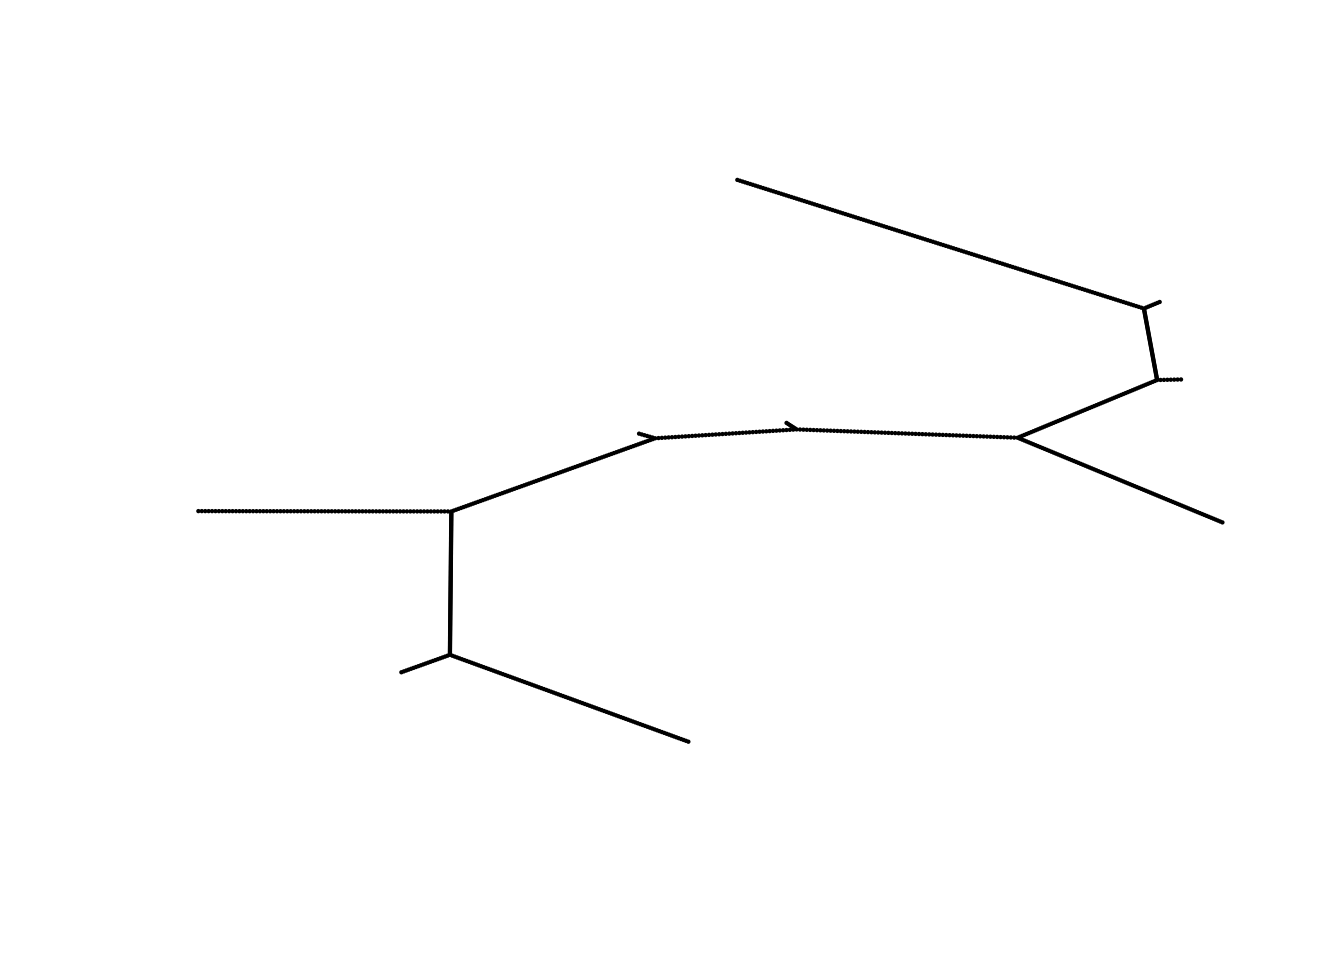
\includegraphics[width=0.7\linewidth]{CellTrails-handbook_files/figure-latex/unnamed-chunk-45-1}

Finally, we set the trajectory layout to the
\emph{\href{http://bioconductor.org/packages/SingleCellExperiment}{SingleCellExperiment}}
object using the \texttt{trajLayout} function. Here, the parameter
\texttt{adjust} indicates if edge lengths should be adjusted, such that
they correspond to the inferred pseudotime.

\begin{Shaded}
\begin{Highlighting}[]
\CommentTok{# Adjust layout and store to object}
\KeywordTok{trajLayout}\NormalTok{(exBundle, }\DataTypeTok{adjust=}\OtherTok{TRUE}\NormalTok{) <-}\StringTok{ }\NormalTok{tl}

\KeywordTok{showTrajInfo}\NormalTok{(exBundle)}
\end{Highlighting}
\end{Shaded}

\begin{verbatim}
## [[ CellTrails ]] 
## logcounts: 183 features, 1008 samples
## Pheno data: 
##   sampleNames: "Cell-1-1" "Cell-1-2" ... "Cell-11-82" (1008)
##   phenoNames: "fm143" "origin" ... "landmark" (4)
## Feature data: 
##   featureNames: "ABCA5" "ARF1" ... "USH2A" (183)
##   rowData: none
## Trajectory data: 
##   trajFeatureNames: "ABCA5" "ARF1" ... "USH2A" (183)
##   latentSpace: 1008 samples, 9 dimensions
##   states: "S1" "S2" ... "S11" (11)
## Trajectories: [Component(#Vertices,Edges)]: 1(10,9)
##   trajSampleNames: "Cell-1-1" "Cell-1-2" ... "Cell-11-82" (896)
##   trajResiduals: MSE=9.9e-03
##   landmarks:  #Branches=7 #Terminals=9 #User=0
##   trajLayout: available
## Trail data: 
##   trailNames: none
\end{verbatim}

\begin{Shaded}
\begin{Highlighting}[]
\CommentTok{# Plot adjusted layout}
\KeywordTok{plot}\NormalTok{(}\KeywordTok{trajLayout}\NormalTok{(exBundle), }\DataTypeTok{axes=}\OtherTok{FALSE}\NormalTok{, }\DataTypeTok{xlab=}\StringTok{""}\NormalTok{, }\DataTypeTok{ylab=}\StringTok{""}\NormalTok{, }\DataTypeTok{pch=}\DecValTok{20}\NormalTok{, }\DataTypeTok{cex=}\NormalTok{.}\DecValTok{25}\NormalTok{)}
\end{Highlighting}
\end{Shaded}

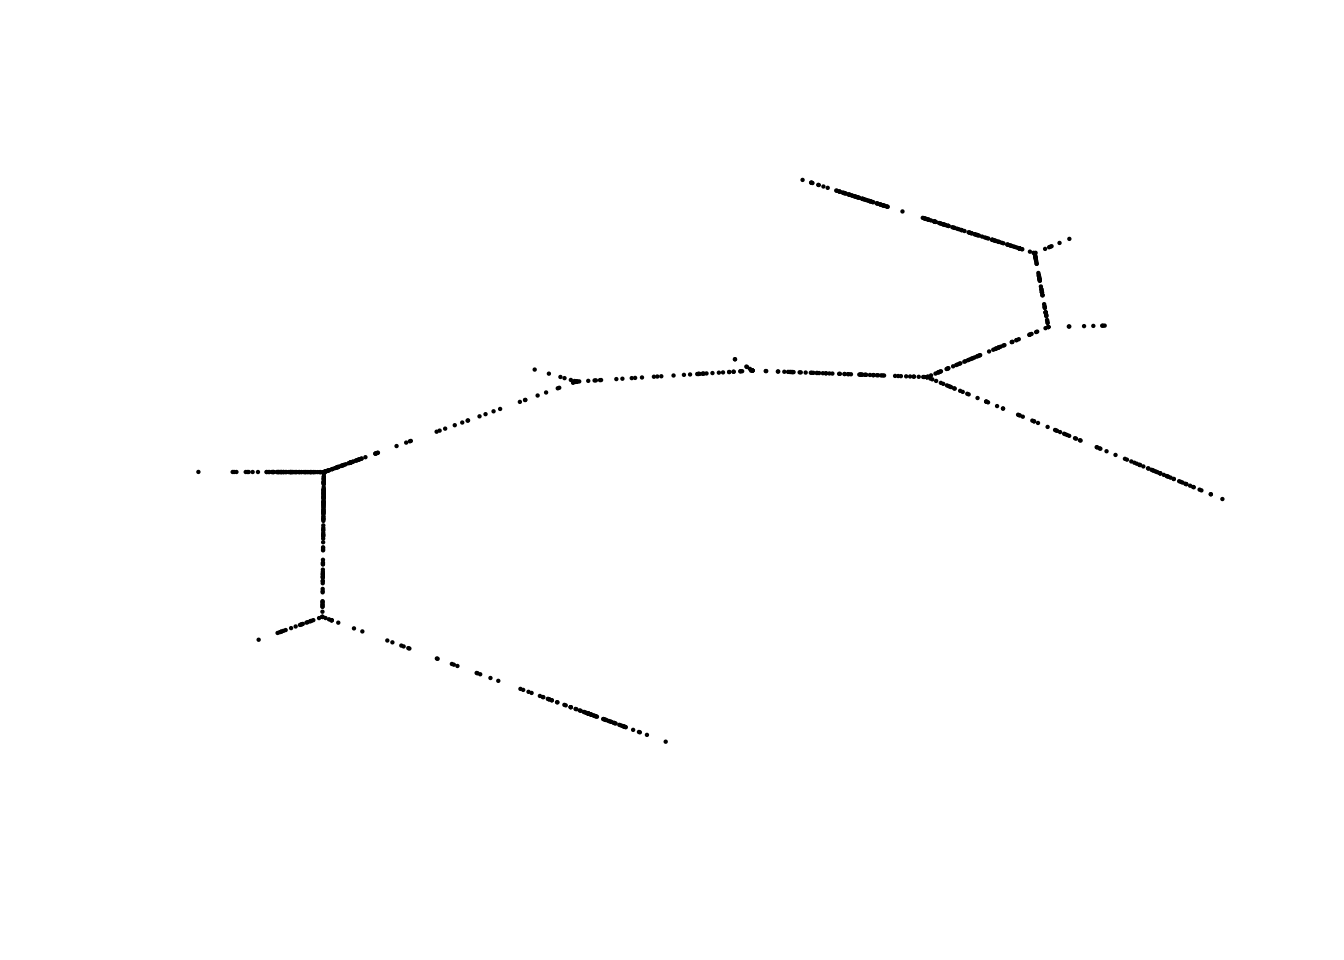
\includegraphics[width=0.7\linewidth]{CellTrails-handbook_files/figure-latex/unnamed-chunk-46-1}

\textbf{Sidenote}. It is not a requirement to use yEd. The trajectory
layout can also be defined by the user otherwise. The minimum
requirement is, that the coordinates of each sample are stored in a
\texttt{data.frame} whose row names correspond to the trajectory sample
names. The sample names can be pulled from the
\emph{\href{http://bioconductor.org/packages/SingleCellExperiment}{SingleCellExperiment}}
object using the function \texttt{trajSampleNames}. The layout can then
be set using the accessor function \texttt{trajLayout} accordingly.

\section{Plot Maps}\label{plot-maps}

After generating the layout, a two-dimensional visualization of the
trajectory can be drawn. Here, the line represents the trajectory and
individual points represent the samples. This plot type either colorizes
individual samples by a metadata label (as available via
\texttt{phenoNames}) or it shows the topography of a given feature's
expression landscape (as available via \texttt{featureNames}). When
metadata are being visualized, the grey line represents the trajectory
and the individual points represent samples. Samples that do not have a
specific metadata label or a missing value are not shown. Let's
visualize how the cellular FM1-43 uptake distributes along the
trajectory:

\begin{Shaded}
\begin{Highlighting}[]
\KeywordTok{plotMap}\NormalTok{(exBundle, }\DataTypeTok{color_by=}\StringTok{"phenoName"}\NormalTok{, }\DataTypeTok{name=}\StringTok{"fm143"}\NormalTok{)}
\end{Highlighting}
\end{Shaded}

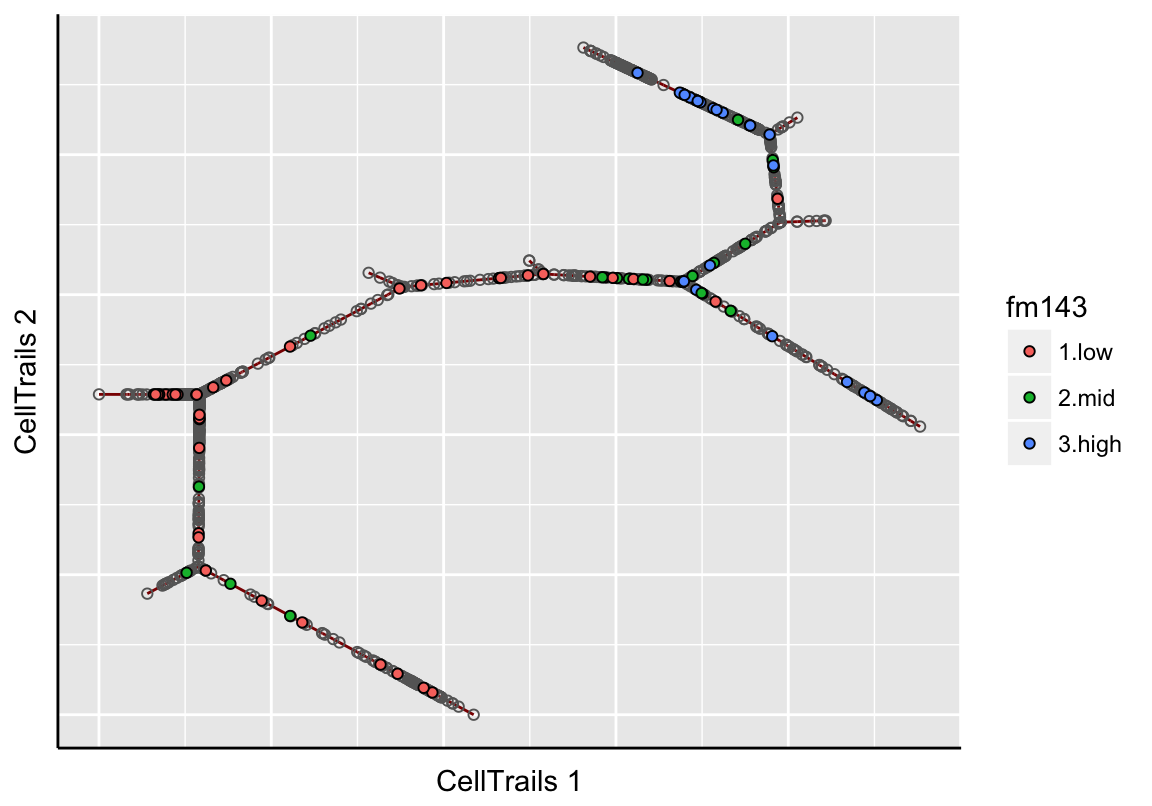
\includegraphics[width=0.7\linewidth]{CellTrails-handbook_files/figure-latex/unnamed-chunk-47-1}

In the topographical plot, a smooth surface is fitted and values are
predicted for a regular grid resulting in the shown map topography; the
red line signifies the trajectory. Let's take a view into the
\emph{ATOH1} expression landscape, an early key transcription factor
during sensory hair cell development:

\begin{Shaded}
\begin{Highlighting}[]
\KeywordTok{plotMap}\NormalTok{(exBundle, }\DataTypeTok{color_by=}\StringTok{"featureName"}\NormalTok{, }\DataTypeTok{name=}\StringTok{"ATOH1"}\NormalTok{, }\DataTypeTok{type=}\StringTok{"surface.fit"}\NormalTok{)}
\end{Highlighting}
\end{Shaded}

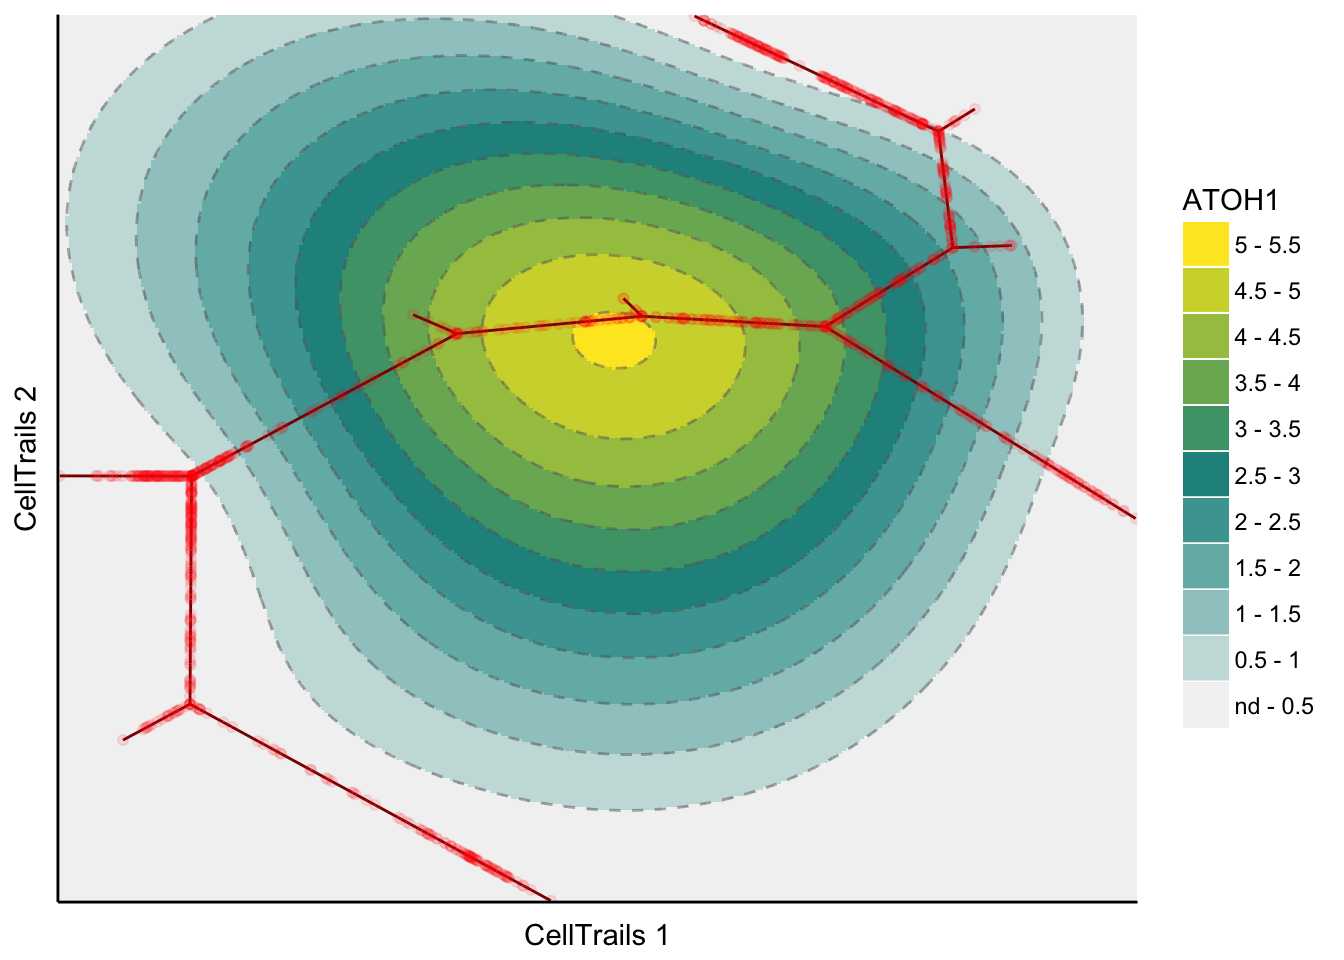
\includegraphics[width=0.7\linewidth]{CellTrails-handbook_files/figure-latex/unnamed-chunk-48-1}

Let's have a look into the standard error of the predicted expression
surface by setting the parameter \texttt{type}.

\begin{Shaded}
\begin{Highlighting}[]
\KeywordTok{plotMap}\NormalTok{(exBundle, }\DataTypeTok{color_by=}\StringTok{"featureName"}\NormalTok{, }\DataTypeTok{name=}\StringTok{"ATOH1"}\NormalTok{, }\DataTypeTok{type=}\StringTok{"surface.se"}\NormalTok{)}
\end{Highlighting}
\end{Shaded}

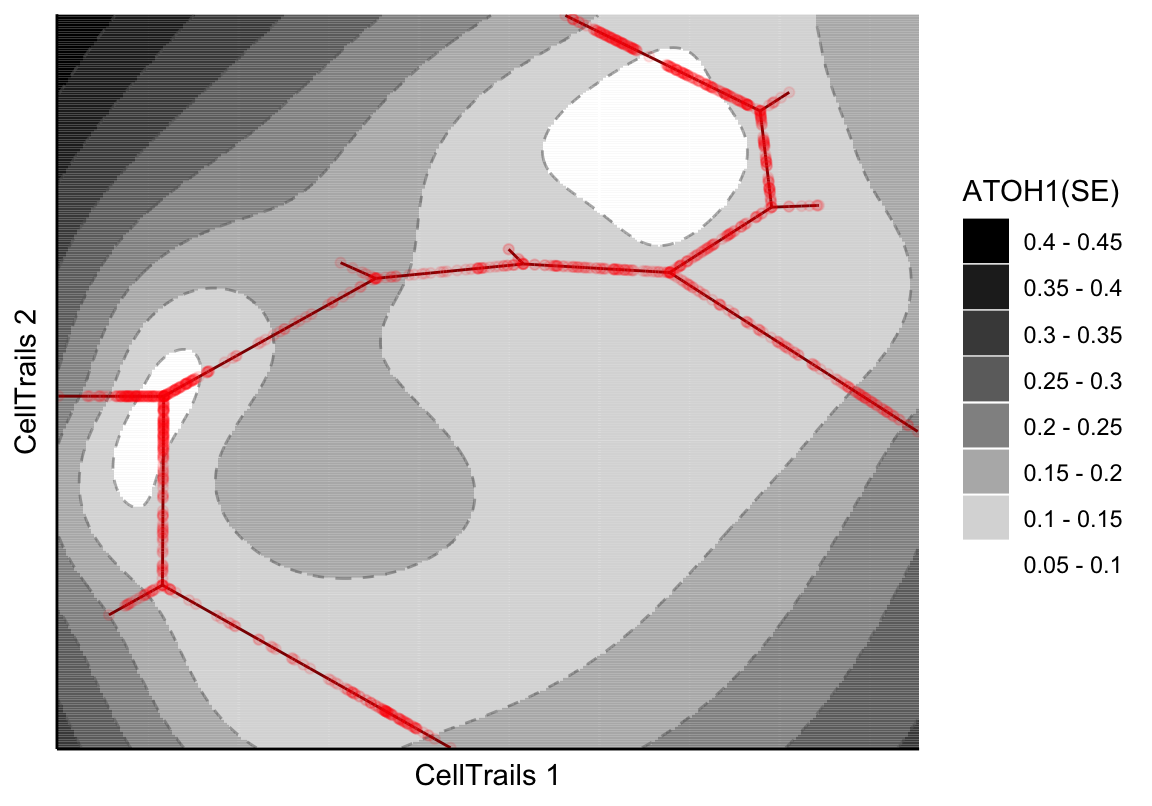
\includegraphics[width=0.7\linewidth]{CellTrails-handbook_files/figure-latex/unnamed-chunk-49-1}

Alternatively, \emph{CellTrails} enables to show the samples only,
instead of the whole fitted expression surface. Here, we have two
options: either the raw expression or the smoothed values.

\begin{Shaded}
\begin{Highlighting}[]
\CommentTok{# Raw}
\KeywordTok{plotMap}\NormalTok{(exBundle, }\DataTypeTok{color_by=}\StringTok{"featureName"}\NormalTok{, }\DataTypeTok{name=}\StringTok{"ATOH1"}\NormalTok{, }\DataTypeTok{type=}\StringTok{"raw"}\NormalTok{)}
\end{Highlighting}
\end{Shaded}

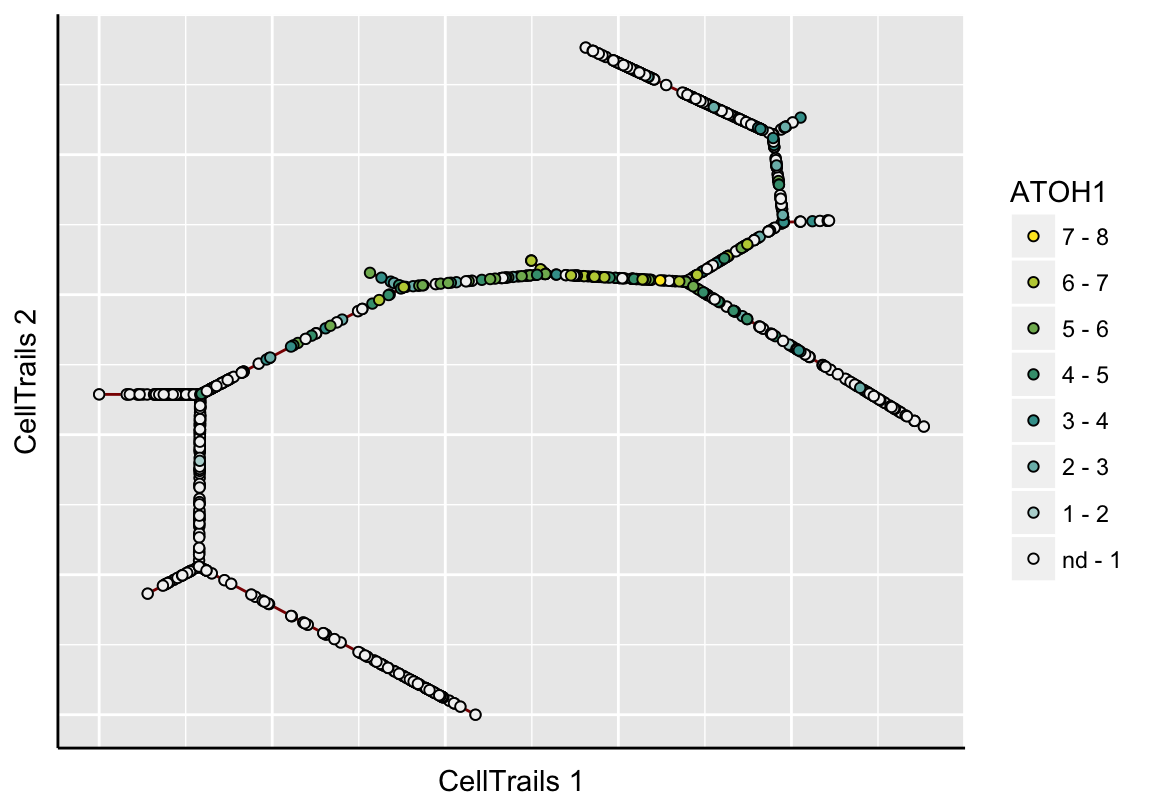
\includegraphics[width=0.7\linewidth]{CellTrails-handbook_files/figure-latex/unnamed-chunk-50-1}

\begin{Shaded}
\begin{Highlighting}[]
\CommentTok{# Smoothed}
\KeywordTok{plotMap}\NormalTok{(exBundle, }\DataTypeTok{color_by=}\StringTok{"featureName"}\NormalTok{, }\DataTypeTok{name=}\StringTok{"ATOH1"}\NormalTok{, }\DataTypeTok{type=}\StringTok{"surface.fit"}\NormalTok{, }
        \DataTypeTok{samples_only=}\OtherTok{TRUE}\NormalTok{)}
\end{Highlighting}
\end{Shaded}

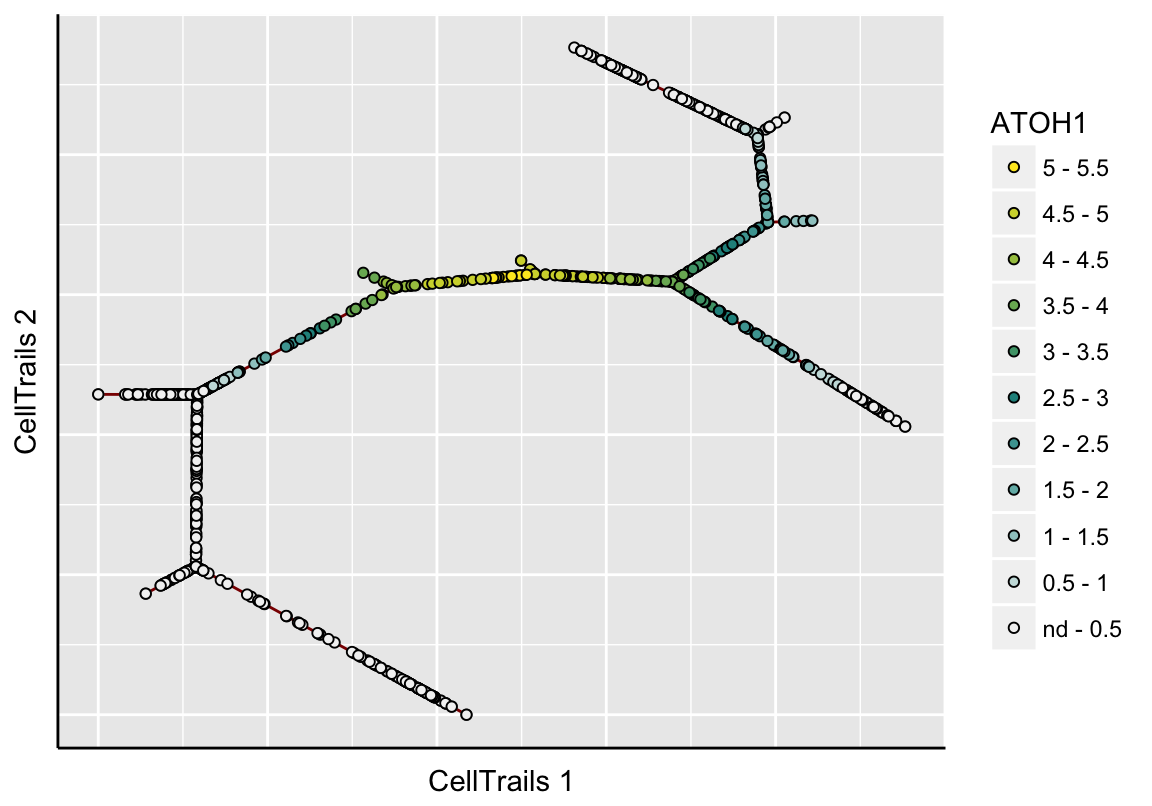
\includegraphics[width=0.7\linewidth]{CellTrails-handbook_files/figure-latex/unnamed-chunk-50-2}

\chapter{Expression Dynamics}\label{expression-dynamics}

During the trajectory fitting process, landmarks are automatically
identified on the trajectory: trail heads (leafs), \emph{H}, and
branching points, \emph{B}. The assigned landmark IDs can be obtained
via \texttt{landmarks}. We use this information to define individual
trails along the trajectory.

\section{Trail Definition}\label{trail-definition}

Trails are usful to infer expression dynamics of features along
subsections of the trajectory. A trail denotes a path between two
landmarks. To be able to properly define a trail, we display the
available landmark points on the trajectory map.

\begin{Shaded}
\begin{Highlighting}[]
\KeywordTok{plotMap}\NormalTok{(exBundle, }\DataTypeTok{color_by=}\StringTok{"phenoName"}\NormalTok{, }\DataTypeTok{name=}\StringTok{"landmark"}\NormalTok{)}
\end{Highlighting}
\end{Shaded}

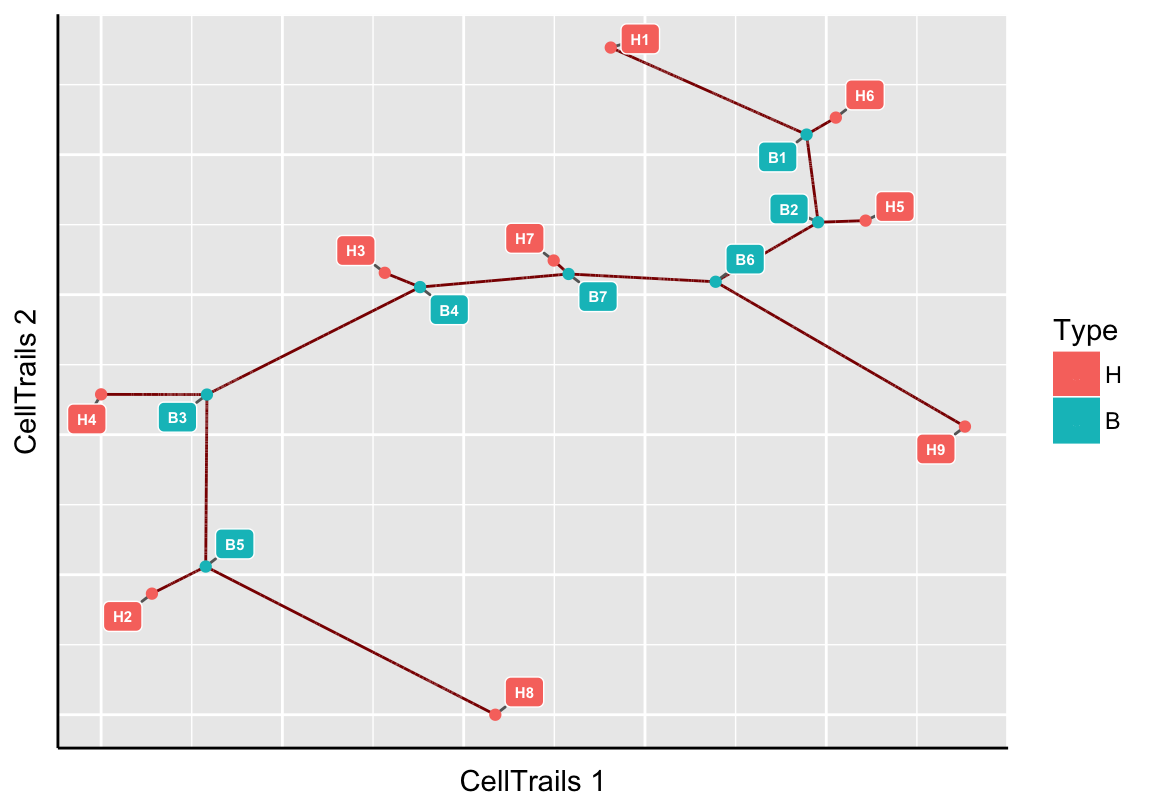
\includegraphics[width=0.7\linewidth]{CellTrails-handbook_files/figure-latex/unnamed-chunk-51-1}

Based on the experimental metainformation and the expression pattern of
marker features, we identified in the original \emph{CellTrails}
publication path \emph{B3} to \emph{H9} as developmental trail toward a
striolar sensory hair bundle morphology, and \emph{B3} to \emph{H1} as
developmental trail toward an extrastriolar bundle morphology. Let's
mark those trails on the map using the function \texttt{addTrail}.

\begin{Shaded}
\begin{Highlighting}[]
\CommentTok{# Define trails}
\NormalTok{exBundle <-}\StringTok{ }\KeywordTok{addTrail}\NormalTok{(exBundle, }\DataTypeTok{from=}\StringTok{"B3"}\NormalTok{, }\DataTypeTok{to=}\StringTok{"H9"}\NormalTok{, }\DataTypeTok{name=}\StringTok{"TrS"}\NormalTok{)}
\NormalTok{exBundle <-}\StringTok{ }\KeywordTok{addTrail}\NormalTok{(exBundle, }\DataTypeTok{from=}\StringTok{"B3"}\NormalTok{, }\DataTypeTok{to=}\StringTok{"H1"}\NormalTok{, }\DataTypeTok{name=}\StringTok{"TrES"}\NormalTok{)}

\KeywordTok{showTrajInfo}\NormalTok{(exBundle)}
\end{Highlighting}
\end{Shaded}

\begin{verbatim}
## [[ CellTrails ]] 
## logcounts: 183 features, 1008 samples
## Pheno data: 
##   sampleNames: "Cell-1-1" "Cell-1-2" ... "Cell-11-82" (1008)
##   phenoNames: "fm143" "origin" ... "landmark" (6)
## Feature data: 
##   featureNames: "ABCA5" "ARF1" ... "USH2A" (183)
##   rowData: none
## Trajectory data: 
##   trajFeatureNames: "ABCA5" "ARF1" ... "USH2A" (183)
##   latentSpace: 1008 samples, 9 dimensions
##   states: "S1" "S2" ... "S11" (11)
## Trajectories: [Component(#Vertices,Edges)]: 1(10,9)
##   trajSampleNames: "Cell-1-1" "Cell-1-2" ... "Cell-11-82" (896)
##   trajResiduals: MSE=9.9e-03
##   landmarks:  #Branches=7 #Terminals=9 #User=0
##   trajLayout: available
## Trail data: 
##   trailNames: "TrS" "TrES" (2)
\end{verbatim}

Next, we want to make sure that the intended trails were extracted by
showing the trajectory map and highlight the defined trails along with
its corresponding pseudotime.

\begin{Shaded}
\begin{Highlighting}[]
\KeywordTok{plotTrail}\NormalTok{(exBundle, }\DataTypeTok{name=}\StringTok{"TrS"}\NormalTok{)}
\end{Highlighting}
\end{Shaded}

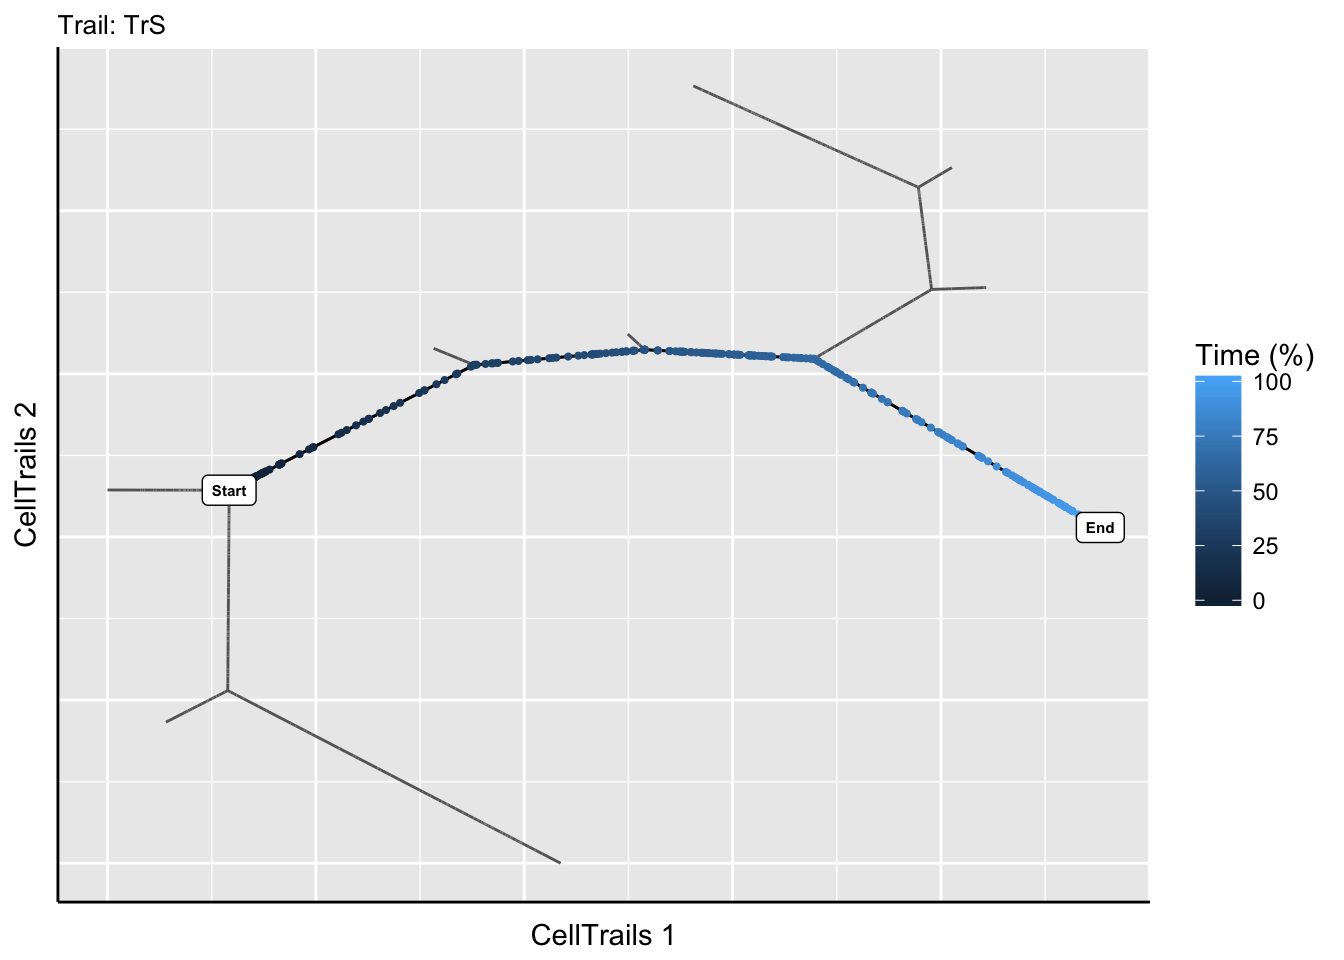
\includegraphics[width=0.7\linewidth]{CellTrails-handbook_files/figure-latex/unnamed-chunk-53-1}

\begin{Shaded}
\begin{Highlighting}[]
\KeywordTok{plotTrail}\NormalTok{(exBundle, }\DataTypeTok{name=}\StringTok{"TrES"}\NormalTok{)}
\end{Highlighting}
\end{Shaded}

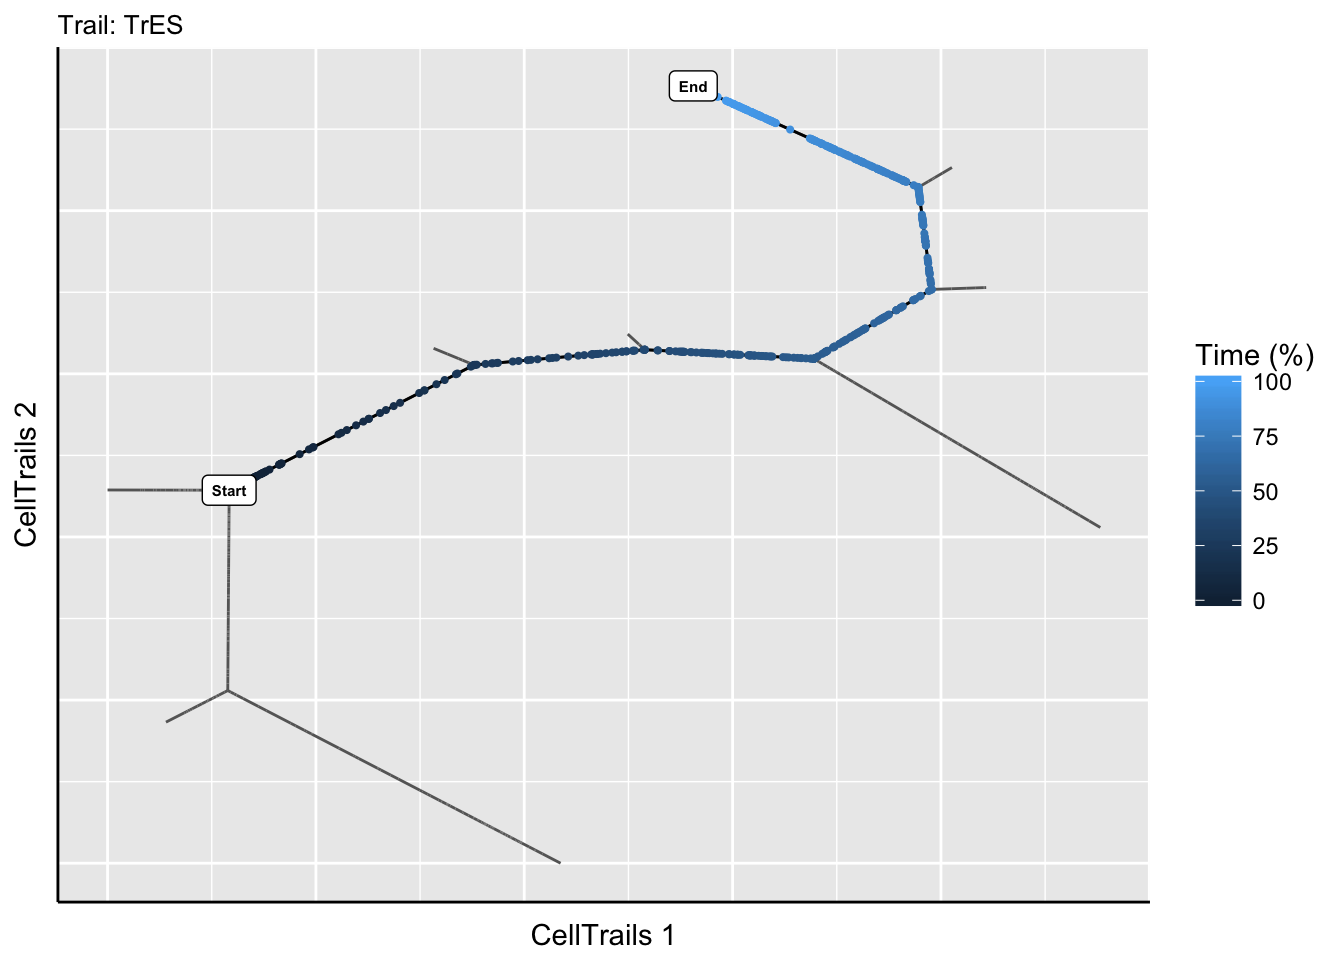
\includegraphics[width=0.7\linewidth]{CellTrails-handbook_files/figure-latex/unnamed-chunk-53-2}

The function \texttt{addTrail} automatically extracts the samples and
their pseudotime along the trail by computing the shortest path between
the trail start and end.

\begin{Shaded}
\begin{Highlighting}[]
\CommentTok{# Get trail names}
\KeywordTok{trailNames}\NormalTok{(exBundle)}
\end{Highlighting}
\end{Shaded}

\begin{verbatim}
## [1] "TrS"  "TrES"
\end{verbatim}

\begin{Shaded}
\begin{Highlighting}[]
\CommentTok{# Get trail pseudotime}
\KeywordTok{trails}\NormalTok{(exBundle)[}\DecValTok{1}\OperatorTok{:}\DecValTok{5}\NormalTok{, ]}
\end{Highlighting}
\end{Shaded}

\begin{verbatim}
## DataFrame with 5 rows and 2 columns
##                TrS      TrES
##          <numeric> <numeric>
## Cell-1-1 0.5776028        NA
## Cell-1-2        NA        NA
## Cell-1-3        NA        NA
## Cell-1-4        NA        NA
## Cell-1-5        NA 0.8723274
\end{verbatim}

The pseudotime information is automatically stored as sample metadata
(see \texttt{phenoNames}). For example, we could plot it on the
lower-dimensional manifold.

\begin{Shaded}
\begin{Highlighting}[]
\CommentTok{# Get trail names}
\KeywordTok{plotManifold}\NormalTok{(exBundle, }\DataTypeTok{color_by=}\StringTok{"phenoName"}\NormalTok{, }\DataTypeTok{name=}\StringTok{"TrS"}\NormalTok{)}
\end{Highlighting}
\end{Shaded}

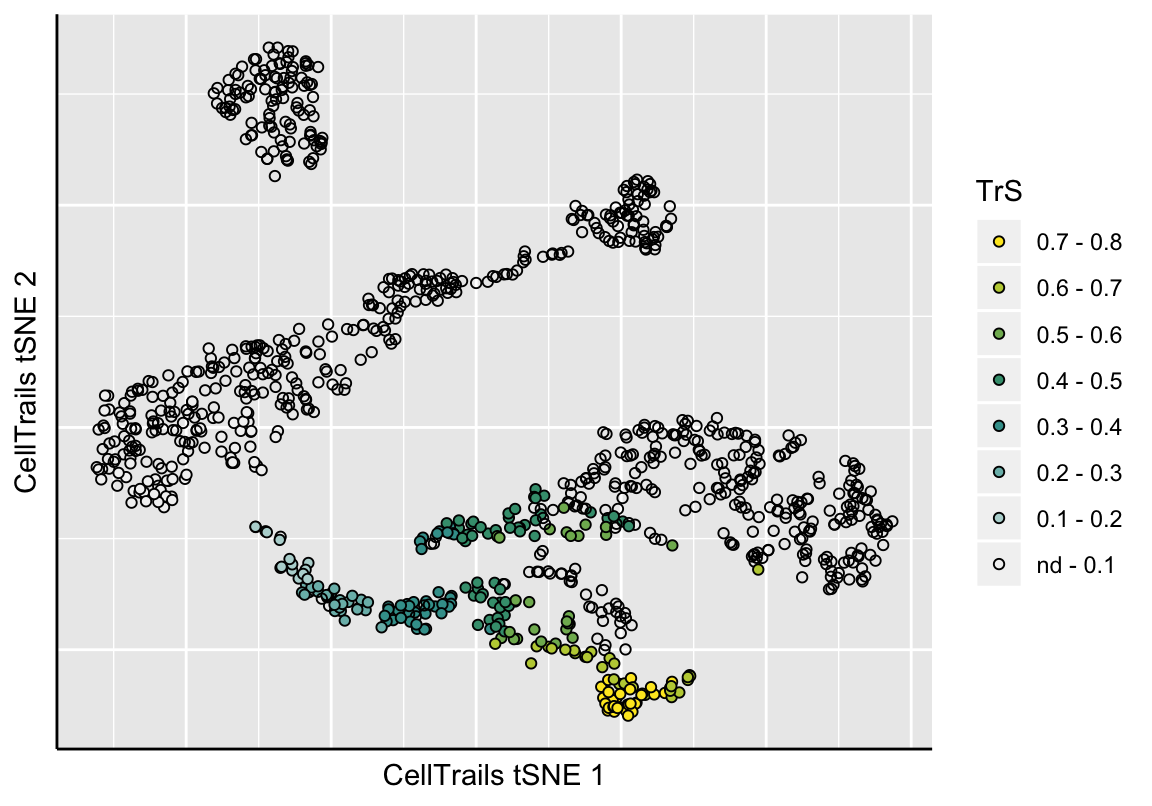
\includegraphics[width=0.7\linewidth]{CellTrails-handbook_files/figure-latex/unnamed-chunk-55-1}

Also, the data is accessible via \texttt{colData} of the
\emph{\href{http://bioconductor.org/packages/SingleCellExperiment}{SingleCellExperiment}}
object and can therefore be analyzed using alternative packages. For
example, colorizing the trail TrS in a principal component analysis
using the \emph{\href{http://bioconductor.org/packages/scater}{scater}}
package \citep{scater}.

\begin{Shaded}
\begin{Highlighting}[]
\NormalTok{## Not run: }
\NormalTok{##library(scater)}
\NormalTok{## End(Not run)}

\CommentTok{# Plot scater PCA with CellTrails pseudotime information}
\NormalTok{scater}\OperatorTok{::}\KeywordTok{plotPCA}\NormalTok{(exBundle, }\DataTypeTok{colour_by=}\StringTok{"CellTrails.TrS"}\NormalTok{)}
\end{Highlighting}
\end{Shaded}

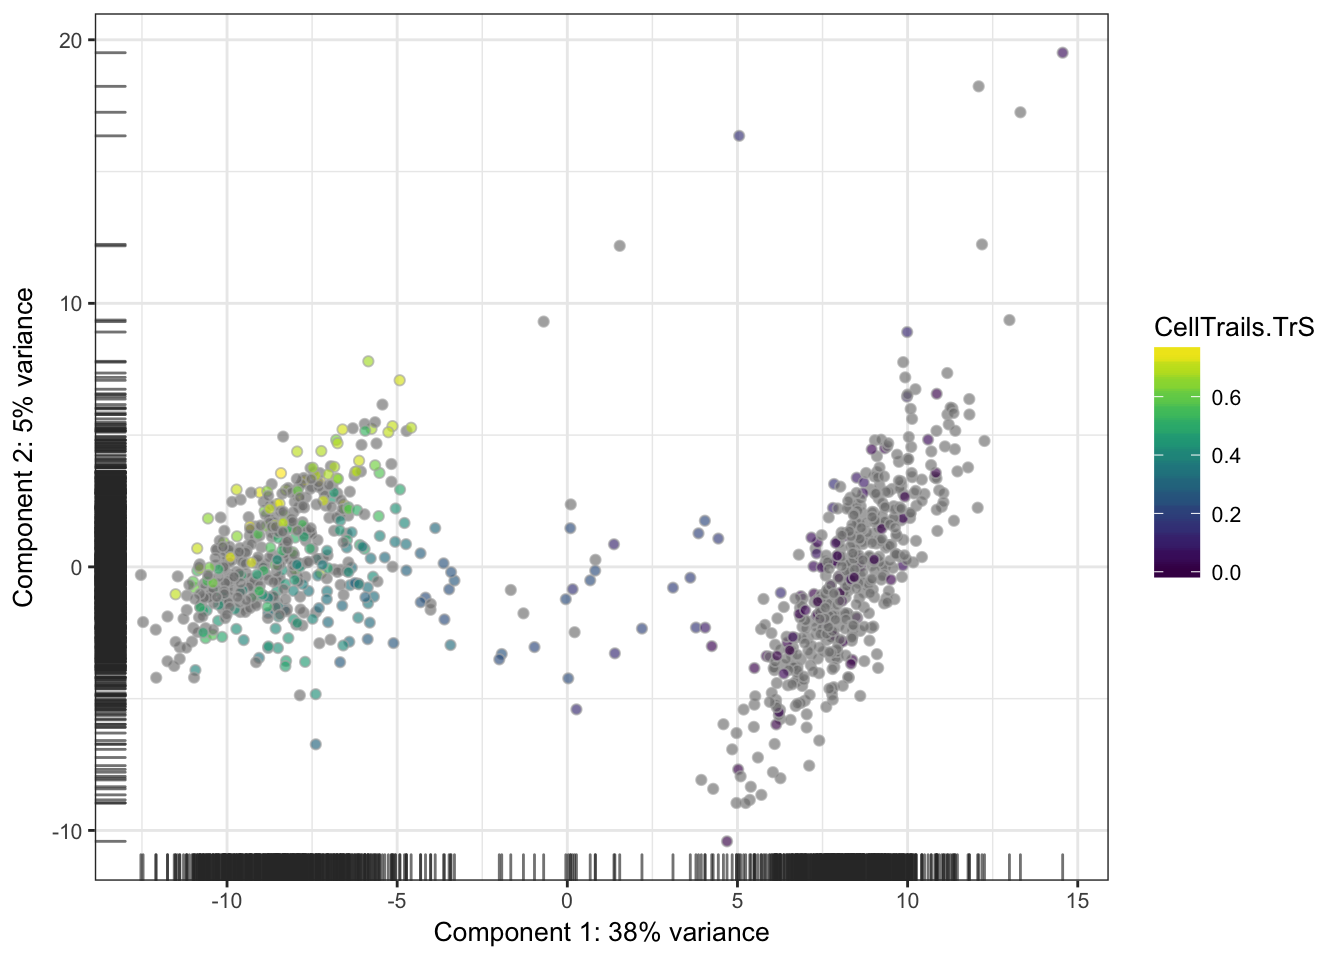
\includegraphics[width=0.7\linewidth]{CellTrails-handbook_files/figure-latex/unnamed-chunk-56-1}

\emph{Please note} that trails can be renamed with
\texttt{trailNames\textless{}-} and removed with \texttt{removeTrail},
respectively. Adding another trail with the same name, will show a
warning message and override the existing definition.

\section{Defining Subtrails}\label{defining-subtrails}

It might be needed to define subtrails if trails overlap. This is
neccessary if the dynamics of one trail are subdynamics of another
trail. Because pseudotime mirrors the location of each datapoint in the
latent space, a significant gap in pseudotime could indicate separate
sample populations. However, these populations have only subtle feature
expression profile differences and were linearly aligned in the latent
space. Since pseudotime can also be interpreted as a function of
transcriptional change, one can argue that these populations undergo the
same expression program (for the selected features), with the small but
distinct difference that samples ordered at the terminal end of the
longer trail up- or down-regulate additional features late during their
maturation. Thus, trails can overlap, while one trail is a subtrail of
the longer trail.

\subsection{Using yEd}\label{using-yed}

\emph{U} landmarks that are needed to define a subtrail can be
determined by the user, as demonstrated in the following.

First, we want to give a rational for selecting a specific node. As
described in the original \emph{CellTrails} article, we found a gap in
pseudotime near the terminal end of trail TrES, which might indicate
that the terminal state can be split, and two trails are actually
overlapping. This gap becomes already quite obvious visually when we
utilize \emph{yEd} to have a closer look into the trajectory graph.
First, we export the graph. By default, nodes are colorized by
\emph{state}.

\begin{Shaded}
\begin{Highlighting}[]
\KeywordTok{write.ygraphml}\NormalTok{(exBundle, }\DataTypeTok{file=}\StringTok{'yourFileName.graphml'}\NormalTok{)}
\end{Highlighting}
\end{Shaded}

Then we open the graphml file in \emph{yEd}. The gap in the purple
colored population is obvious:

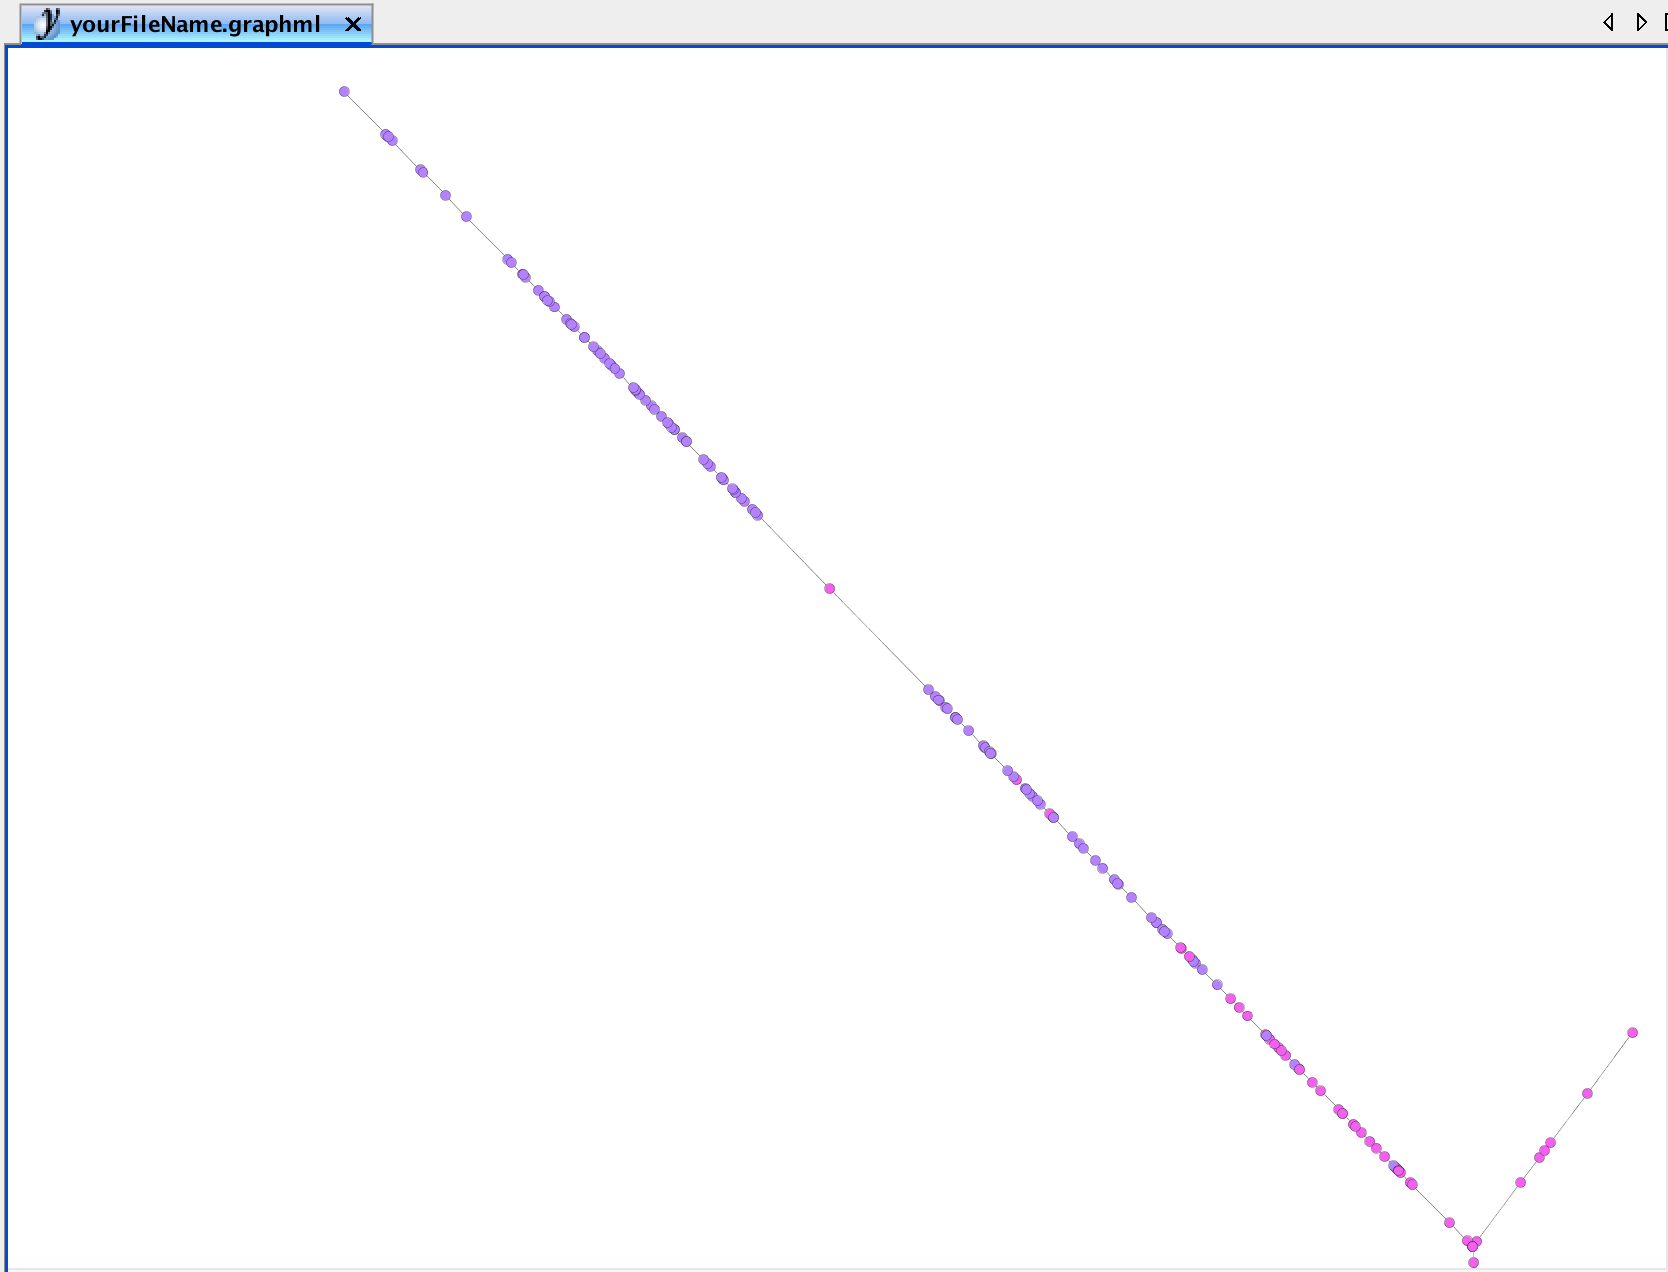
\includegraphics[width=0.7\linewidth]{img/yEd_7}

To indicate this sample as landmark, we simply change the shape of this
node. This can be any shape, but not \emph{ellipse}, which is used as
default for other nodes. The shape can be changed using the
\emph{Properties View} panel on the right border of the \emph{yEd}
application.

\includegraphics[width=0.7\linewidth]{img/yEd_8}

After saving the layout, it can be reimported to \emph{CellTrails} and
the landmark can be used to define the subtrail:

\begin{Shaded}
\begin{Highlighting}[]
\CommentTok{# Trail Identification}
\KeywordTok{plotMap}\NormalTok{(exBundle, }\DataTypeTok{color_by=}\StringTok{"phenoName"}\NormalTok{, }\DataTypeTok{name=}\StringTok{"landmark"}\NormalTok{)}
\end{Highlighting}
\end{Shaded}

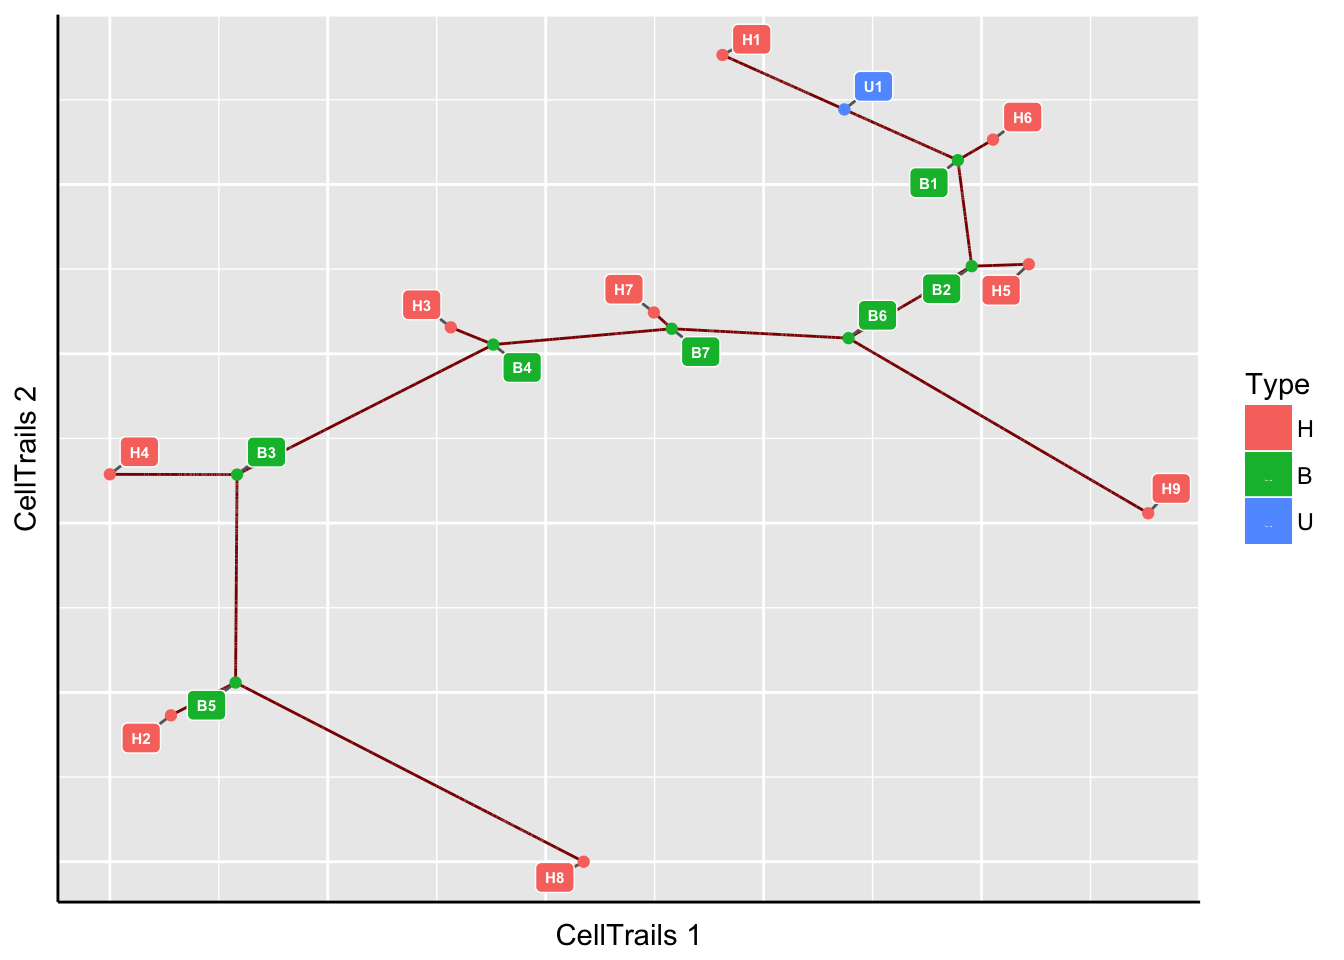
\includegraphics[width=0.7\linewidth]{CellTrails-handbook_files/figure-latex/unnamed-chunk-61-1}

\begin{Shaded}
\begin{Highlighting}[]
\NormalTok{exBundle <-}\StringTok{ }\KeywordTok{addTrail}\NormalTok{(exBundle, }\DataTypeTok{from=}\StringTok{"B3"}\NormalTok{, }\DataTypeTok{to=}\StringTok{"U1"}\NormalTok{, }\DataTypeTok{name=}\StringTok{"TrES*"}\NormalTok{)}
\KeywordTok{plotTrail}\NormalTok{(exBundle, }\DataTypeTok{name=}\StringTok{"TrES*"}\NormalTok{)}
\end{Highlighting}
\end{Shaded}

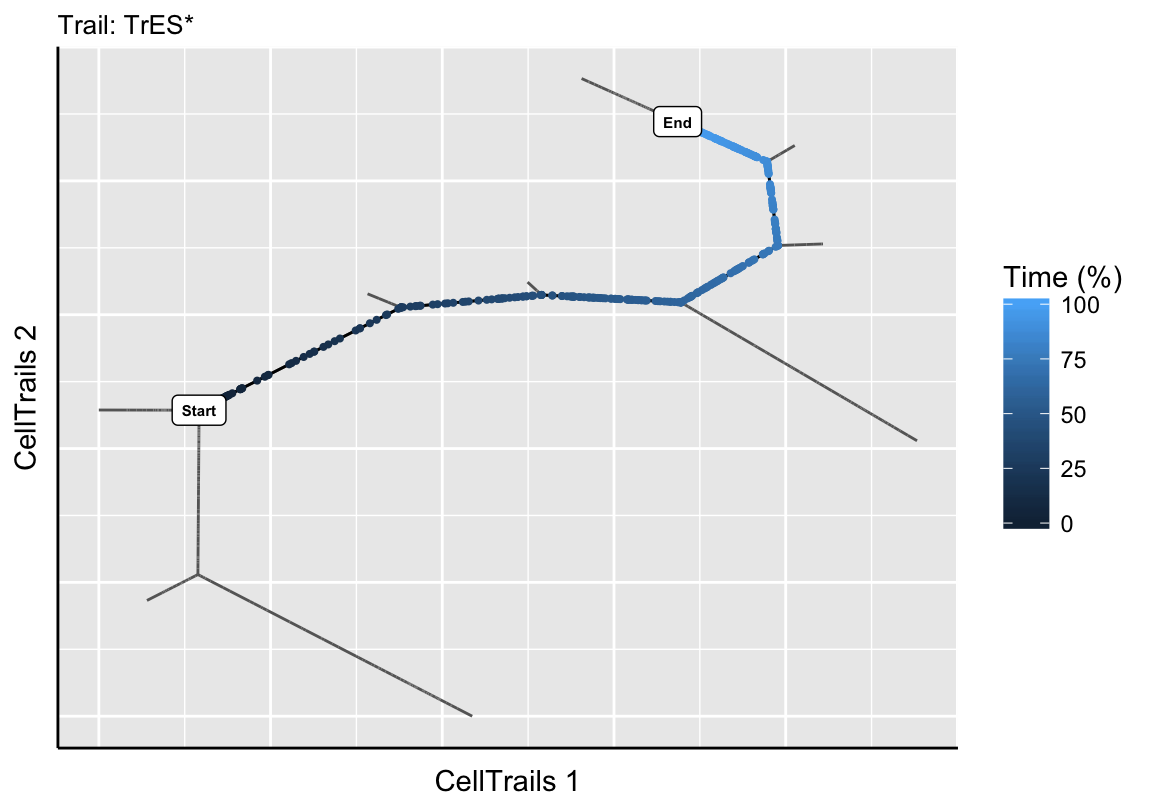
\includegraphics[width=0.7\linewidth]{CellTrails-handbook_files/figure-latex/unnamed-chunk-61-2}

\begin{Shaded}
\begin{Highlighting}[]
\KeywordTok{showTrajInfo}\NormalTok{(exBundle)}
\end{Highlighting}
\end{Shaded}

\begin{verbatim}
## [[ CellTrails ]] 
## logcounts: 183 features, 1008 samples
## Pheno data: 
##   sampleNames: "Cell-1-1" "Cell-1-2" ... "Cell-11-82" (1008)
##   phenoNames: "fm143" "origin" ... "landmark" (7)
## Feature data: 
##   featureNames: "ABCA5" "ARF1" ... "USH2A" (183)
##   rowData: none
## Trajectory data: 
##   trajFeatureNames: "ABCA5" "ARF1" ... "USH2A" (183)
##   latentSpace: 1008 samples, 9 dimensions
##   states: "S1" "S2" ... "S11" (11)
## Trajectories: [Component(#Vertices,Edges)]: 1(10,9)
##   trajSampleNames: "Cell-1-1" "Cell-1-2" ... "Cell-11-82" (896)
##   trajResiduals: MSE=9.9e-03
##   landmarks:  #Branches=7 #Terminals=9 #User=1
##   trajLayout: available
## Trail data: 
##   trailNames: "TrS" "TrES" "TrES*" (3)
\end{verbatim}

\emph{Please note} that the trajectory graph can also be exported having
all landmarks highlighted. This is particulary helpful if user-defined
landmarks need to be changed.

\begin{Shaded}
\begin{Highlighting}[]
\CommentTok{# Export Trajectory Graph Layout with sample names}
\KeywordTok{write.ygraphml}\NormalTok{(exBundle, }\DataTypeTok{file=}\StringTok{'yourFileName.graphml'}\NormalTok{, }
               \DataTypeTok{color_by=}\StringTok{"phenoName"}\NormalTok{, }\DataTypeTok{name=}\StringTok{"landmark"}\NormalTok{, }
               \DataTypeTok{node_label=}\StringTok{"landmark"}\NormalTok{)}
\end{Highlighting}
\end{Shaded}

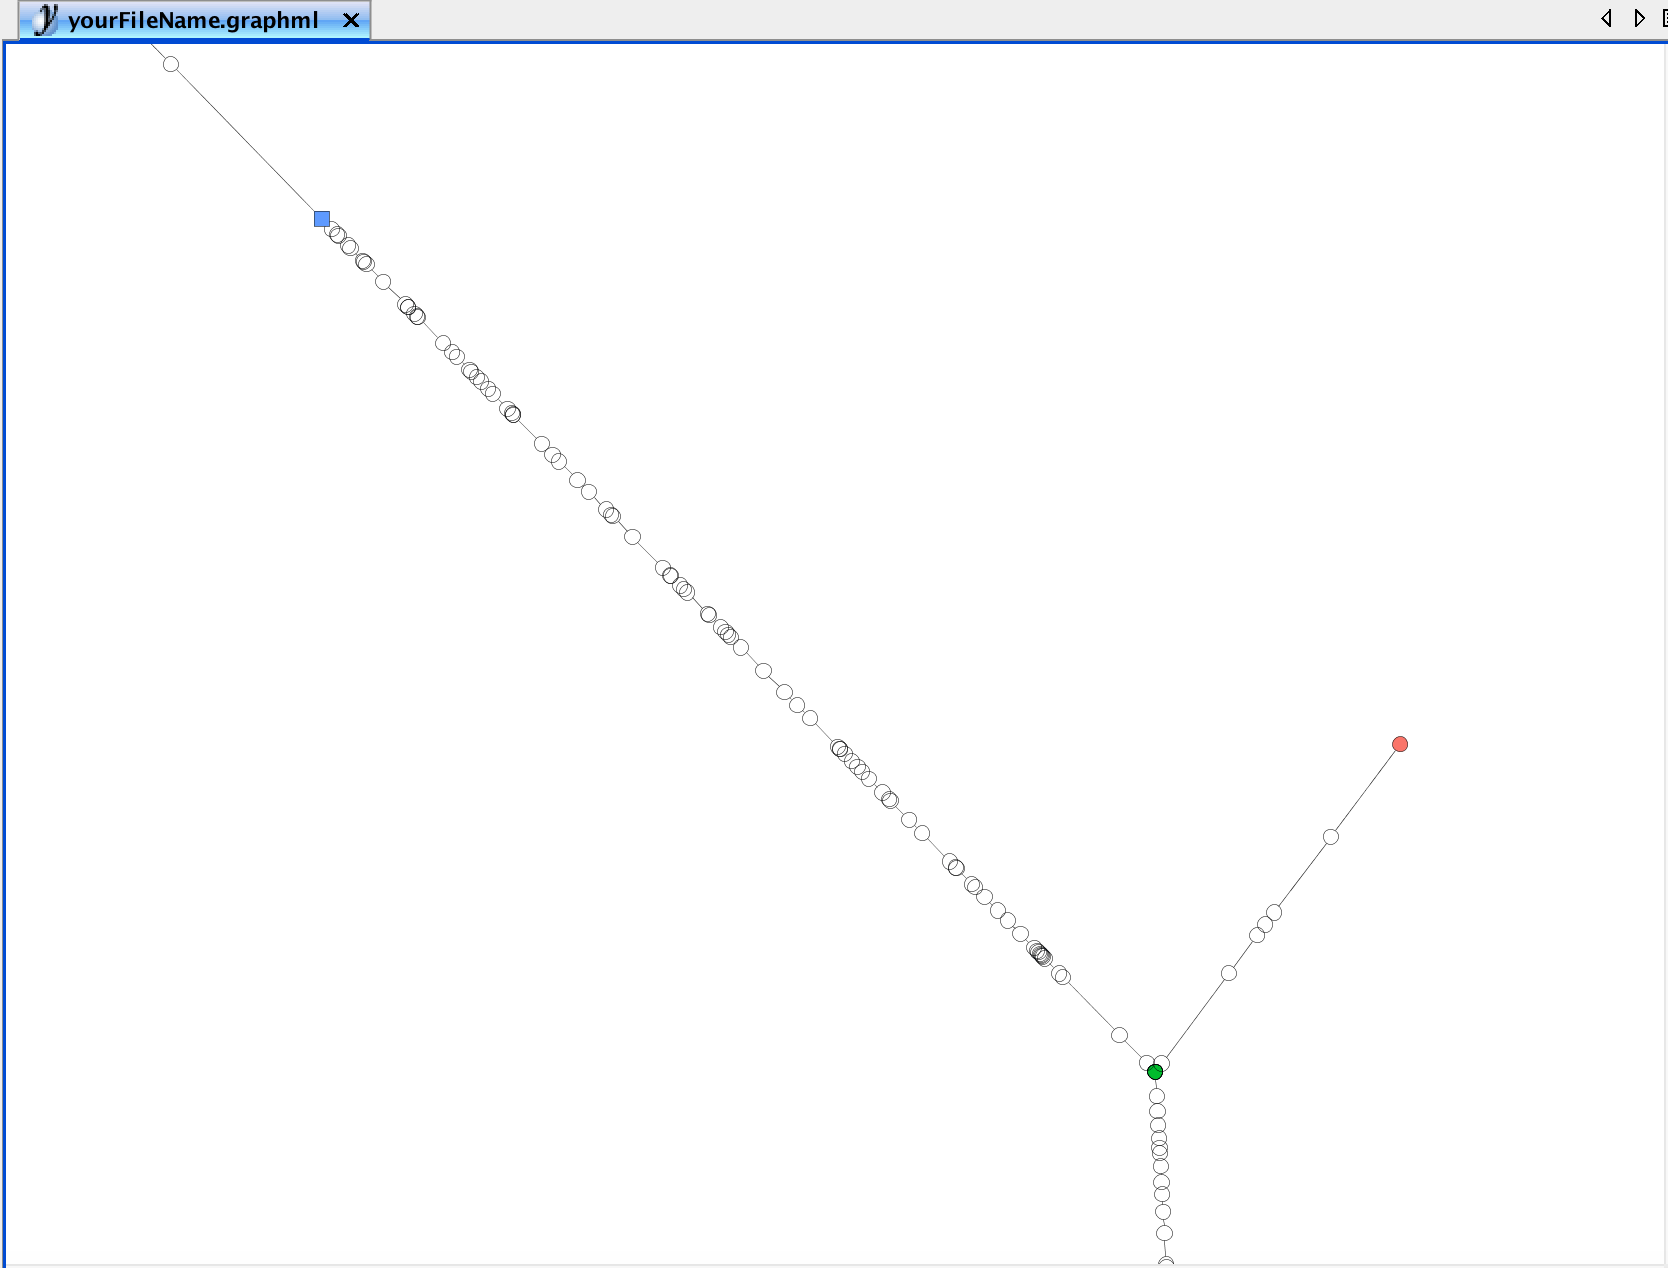
\includegraphics[width=0.7\linewidth]{img/yEd_9}

Here, blue nodes denote user-defined landmarks, green nodes are
branching points and red nodes are leafs. Landmark IDs, as listed by
\texttt{landmarks}, are indicated as node names, respectively.

\subsection{Using R}\label{using-r}

A visual and empiric identification of user-defined landmarks can be
helpful, but scientifically more appropriate is a statistical approach.
For this purpose we analyze the distribution of all lagged differences
along trail TrES. Here, we make use of the pseudotime information of
each trail, respectively.

\begin{Shaded}
\begin{Highlighting}[]
\CommentTok{# Extract pseudotime of TrES}
\NormalTok{ptime <-}\StringTok{ }\KeywordTok{trails}\NormalTok{(exBundle)[, }\StringTok{"TrES"}\NormalTok{]}

\CommentTok{# Subset SingleCellExperiment set}
\CommentTok{# to samples which are part of trail TrES}
\NormalTok{trES <-}\StringTok{ }\NormalTok{exBundle[, }\OperatorTok{!}\KeywordTok{is.na}\NormalTok{(ptime)]}

\CommentTok{# Order samples by pseudotime}
\NormalTok{o <-}\StringTok{ }\KeywordTok{order}\NormalTok{(}\KeywordTok{trails}\NormalTok{(trES)[, }\StringTok{"TrES"}\NormalTok{])}
\NormalTok{trES <-}\StringTok{ }\NormalTok{trES[, o]}
\NormalTok{ptime <-}\StringTok{ }\KeywordTok{trails}\NormalTok{(trES)[, }\StringTok{"TrES"}\NormalTok{]}
\KeywordTok{names}\NormalTok{(ptime) <-}\StringTok{ }\KeywordTok{colnames}\NormalTok{(trES)}

\CommentTok{# Lagged pseudotime values per state}
\NormalTok{ptime_states <-}\StringTok{ }\KeywordTok{split}\NormalTok{(ptime, }\KeywordTok{states}\NormalTok{(trES))}
\NormalTok{lptime <-}\StringTok{ }\KeywordTok{lapply}\NormalTok{(ptime_states, }
                 \ControlFlowTok{function}\NormalTok{(x)\{y <-}\StringTok{ }\KeywordTok{diff}\NormalTok{(}\KeywordTok{sort}\NormalTok{(x)); y[}\OperatorTok{-}\KeywordTok{length}\NormalTok{(y)]\})}

\NormalTok{bp <-}\StringTok{ }\KeywordTok{boxplot}\NormalTok{(lptime, }\DataTypeTok{horizontal=}\OtherTok{TRUE}\NormalTok{, }
              \DataTypeTok{ylab=}\StringTok{"State"}\NormalTok{, }\DataTypeTok{xlab=}\StringTok{"Pseudotime delta"}\NormalTok{, }\DataTypeTok{las=}\DecValTok{2}\NormalTok{)}
\end{Highlighting}
\end{Shaded}

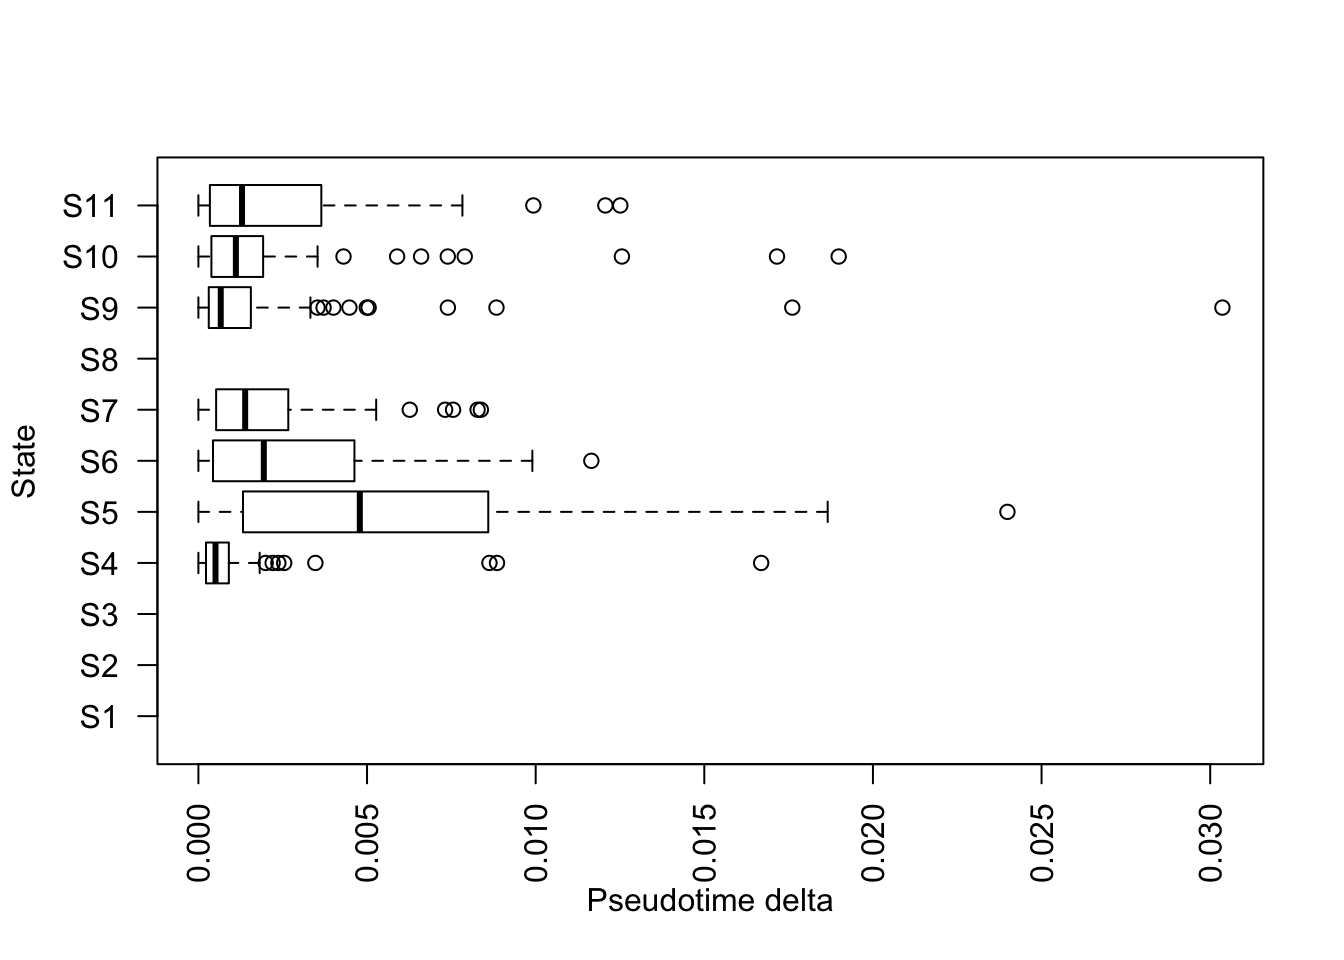
\includegraphics[width=0.7\linewidth]{CellTrails-handbook_files/figure-latex/unnamed-chunk-66-1}

The boxplot statistics indicate that there is a strong outlier in state
S9 (which is termed state \emph{i} in the original \emph{CellTrails}
article). Let's extract the sample right before the leap.

\begin{Shaded}
\begin{Highlighting}[]
\NormalTok{leap <-}\StringTok{ }\NormalTok{lptime}\OperatorTok{$}\NormalTok{S9[}\KeywordTok{which.max}\NormalTok{(lptime}\OperatorTok{$}\NormalTok{S9) }\OperatorTok{-}\StringTok{ }\DecValTok{1}\NormalTok{]}
\KeywordTok{names}\NormalTok{(leap)}
\end{Highlighting}
\end{Shaded}

\begin{verbatim}
## [1] "Cell-8-57"
\end{verbatim}

The function \texttt{userLandmarks\textless{}-} enables us to
(re-)define the set of user landmarks.

\begin{Shaded}
\begin{Highlighting}[]
\KeywordTok{userLandmarks}\NormalTok{(exBundle) <-}\StringTok{ }\KeywordTok{names}\NormalTok{(leap)}

\CommentTok{# Trail Identification}
\KeywordTok{plotMap}\NormalTok{(exBundle, }\DataTypeTok{color_by=}\StringTok{"phenoName"}\NormalTok{, }\DataTypeTok{name=}\StringTok{"landmark"}\NormalTok{)}
\end{Highlighting}
\end{Shaded}

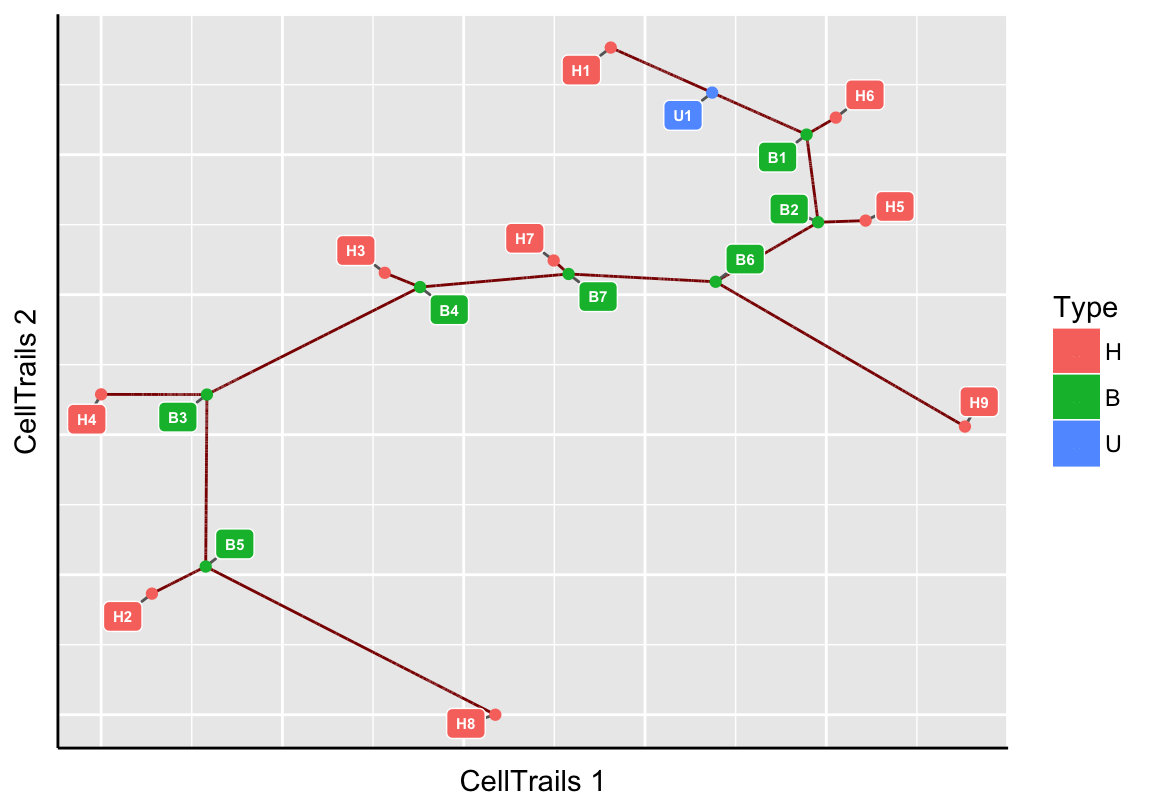
\includegraphics[width=0.7\linewidth]{CellTrails-handbook_files/figure-latex/unnamed-chunk-68-1}

\begin{Shaded}
\begin{Highlighting}[]
\NormalTok{exBundle <-}\StringTok{ }\KeywordTok{addTrail}\NormalTok{(exBundle, }\DataTypeTok{from=}\StringTok{"B3"}\NormalTok{, }\DataTypeTok{to=}\StringTok{"U1"}\NormalTok{, }\DataTypeTok{name=}\StringTok{"TrES*"}\NormalTok{)}
\KeywordTok{plotTrail}\NormalTok{(exBundle, }\DataTypeTok{name=}\StringTok{"TrES*"}\NormalTok{)}
\end{Highlighting}
\end{Shaded}

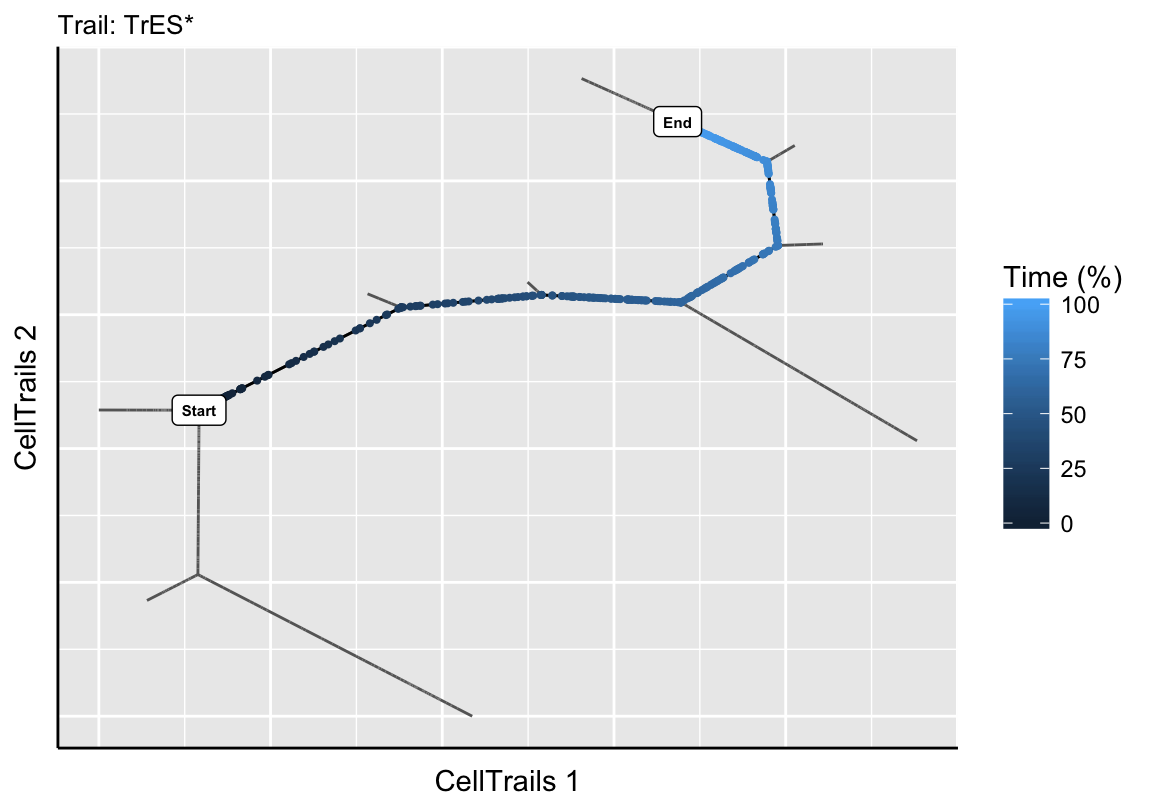
\includegraphics[width=0.7\linewidth]{CellTrails-handbook_files/figure-latex/unnamed-chunk-68-2}

\begin{Shaded}
\begin{Highlighting}[]
\KeywordTok{showTrajInfo}\NormalTok{(exBundle)}
\end{Highlighting}
\end{Shaded}

\begin{verbatim}
## [[ CellTrails ]] 
## logcounts: 183 features, 1008 samples
## Pheno data: 
##   sampleNames: "Cell-1-1" "Cell-1-2" ... "Cell-11-82" (1008)
##   phenoNames: "fm143" "origin" ... "landmark" (7)
## Feature data: 
##   featureNames: "ABCA5" "ARF1" ... "USH2A" (183)
##   rowData: none
## Trajectory data: 
##   trajFeatureNames: "ABCA5" "ARF1" ... "USH2A" (183)
##   latentSpace: 1008 samples, 9 dimensions
##   states: "S1" "S2" ... "S11" (11)
## Trajectories: [Component(#Vertices,Edges)]: 1(10,9)
##   trajSampleNames: "Cell-1-1" "Cell-1-2" ... "Cell-11-82" (896)
##   trajResiduals: MSE=9.9e-03
##   landmarks:  #Branches=7 #Terminals=9 #User=1
##   trajLayout: available
## Trail data: 
##   trailNames: "TrS" "TrES" "TrES*" (3)
\end{verbatim}

\emph{Please note} that all user-defined landmarks can be removed using
\texttt{userLandmarks(exBundle)\ \textless{}-\ NULL}.

\section{Inference of Dynamics}\label{inference-of-dynamics}

\emph{CellTrails} defines pseudotime as the geodesic distance of each
node of the trail from the start node. To learn the expression level of
a feature as a function of pseudotime, \emph{CellTrails} used
generalized additive models (GAM) with a single smoothing term with five
basis dimensions. Here, for each feature, \emph{CellTrails} introduces
prior weights for each observation to lower the confounding effect of
missing data to the maximum-likelihood-based fitting process.

Feature expression as a function of pseudotime along an individual trail
can be plotted with the \texttt{plotDynamic} function. This results in
the fitted dynamic function (= black line) and the individual expression
per sample (= points represent samples colored by their state
membership). For example, the expression of the calcium buffer
\emph{CALB2} during extrastriolar hair cell development can be displayed
as follows:

\begin{Shaded}
\begin{Highlighting}[]
\KeywordTok{plotDynamic}\NormalTok{(exBundle, }\DataTypeTok{feature_name=}\StringTok{"CALB2"}\NormalTok{, }\DataTypeTok{trail_name=}\StringTok{"TrES"}\NormalTok{)}
\end{Highlighting}
\end{Shaded}

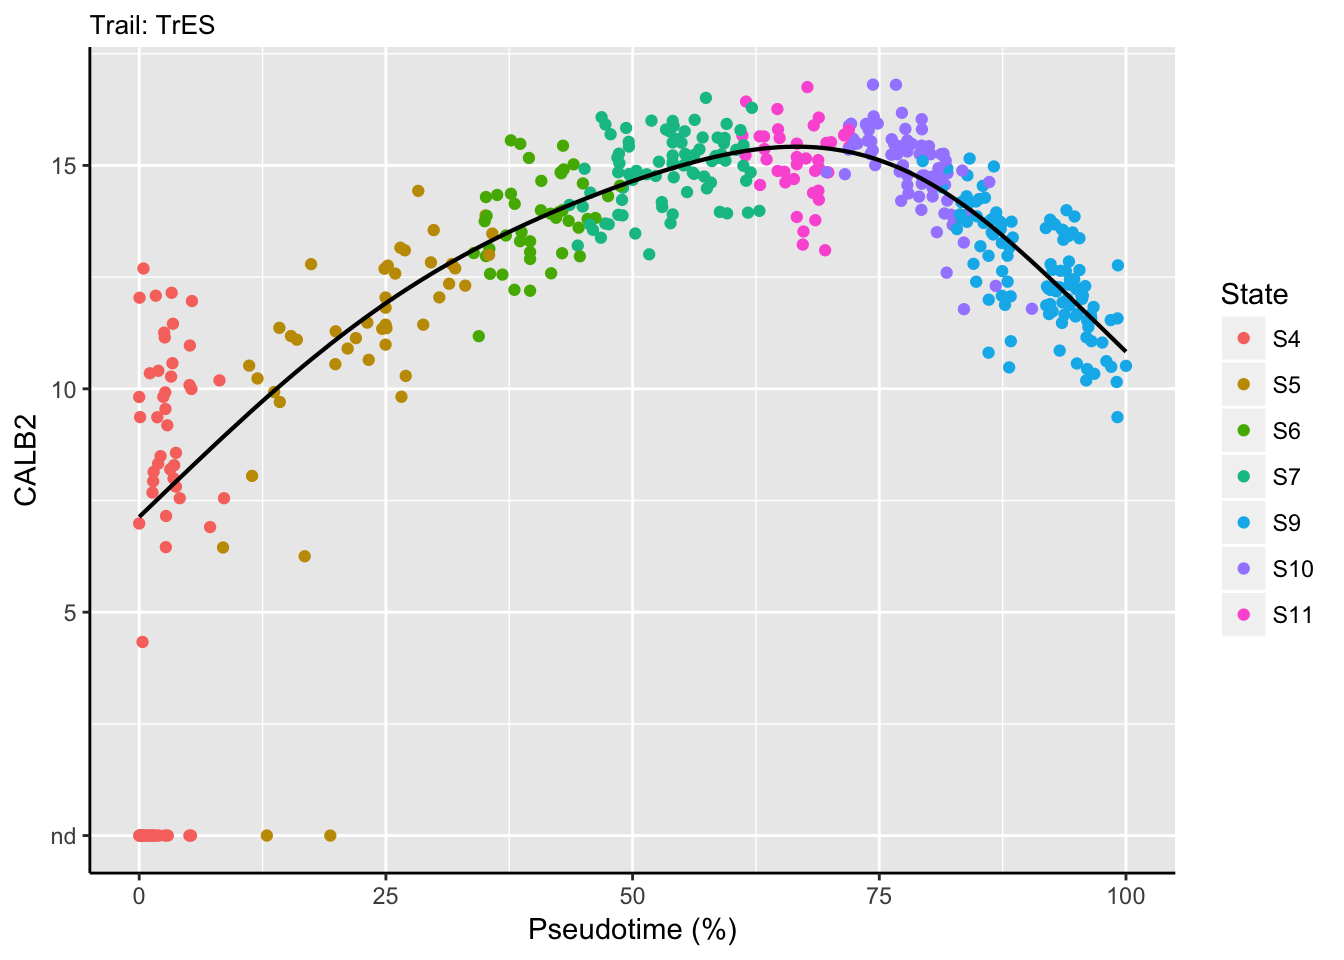
\includegraphics[width=0.7\linewidth]{CellTrails-handbook_files/figure-latex/unnamed-chunk-69-1}

\emph{Please note} that the fitting function automatically scales
pseudotime between 0 and 100\% for each trail.

The fit information can be extracted via function \texttt{fitDynamic}
and used for further downstream analyses:

\begin{Shaded}
\begin{Highlighting}[]
\NormalTok{fit <-}\StringTok{ }\KeywordTok{fitDynamic}\NormalTok{(exBundle, }\DataTypeTok{trail_name=}\StringTok{"TrES"}\NormalTok{, }\DataTypeTok{feature_name=}\StringTok{"CALB2"}\NormalTok{)}

\KeywordTok{summary}\NormalTok{(fit)}
\end{Highlighting}
\end{Shaded}

\begin{verbatim}
##            Length Class  Mode   
## pseudotime 470    -none- numeric
## expression 470    -none- numeric
## gam         52    gam    list
\end{verbatim}

\begin{Shaded}
\begin{Highlighting}[]
\KeywordTok{range}\NormalTok{(fit}\OperatorTok{$}\NormalTok{pseudotime)}
\end{Highlighting}
\end{Shaded}

\begin{verbatim}
## [1] 0 1
\end{verbatim}

\begin{Shaded}
\begin{Highlighting}[]
\KeywordTok{range}\NormalTok{(fit}\OperatorTok{$}\NormalTok{expression)}
\end{Highlighting}
\end{Shaded}

\begin{verbatim}
## [1]  7.131096 15.419633
\end{verbatim}

\begin{Shaded}
\begin{Highlighting}[]
\CommentTok{# Predict expression at 0%, 25%, 50%, 75% and 100% of pseudotime}
\NormalTok{timepoints <-}\StringTok{ }\KeywordTok{data.frame}\NormalTok{(}\DataTypeTok{x=}\KeywordTok{c}\NormalTok{(}\StringTok{"0%"}\NormalTok{=}\DecValTok{0}\NormalTok{, }\StringTok{"25%"}\NormalTok{=.}\DecValTok{25}\NormalTok{, }\StringTok{"50%"}\NormalTok{=.}\DecValTok{5}\NormalTok{, }\StringTok{"75%"}\NormalTok{=.}\DecValTok{75}\NormalTok{, }\StringTok{"100%"}\NormalTok{=}\DecValTok{1}\NormalTok{))}
\KeywordTok{predict}\NormalTok{(fit}\OperatorTok{$}\NormalTok{gam, }\DataTypeTok{newdata=}\NormalTok{timepoints)}
\end{Highlighting}
\end{Shaded}

\begin{verbatim}
##        0%       25%       50%       75%      100% 
##  7.131096 11.917652 14.649184 15.117750 10.831007
\end{verbatim}

\section{Dynamic Comparison: Within
Trails}\label{dynamic-comparison-within-trails}

\emph{CellTrails} allows the analysis and comparison of the expression
of multiple features along a single trail. For example, the expression
dynamics of the acting crosslinkers \emph{FSCN1} and \emph{FSCN2} can be
displayed in a single plot as follows:

\begin{Shaded}
\begin{Highlighting}[]
\KeywordTok{plotDynamic}\NormalTok{(exBundle, }\DataTypeTok{feature_name=}\KeywordTok{c}\NormalTok{(}\StringTok{"FSCN1"}\NormalTok{, }\StringTok{"FSCN2"}\NormalTok{), }\DataTypeTok{trail_name=}\StringTok{"TrES"}\NormalTok{)}
\end{Highlighting}
\end{Shaded}

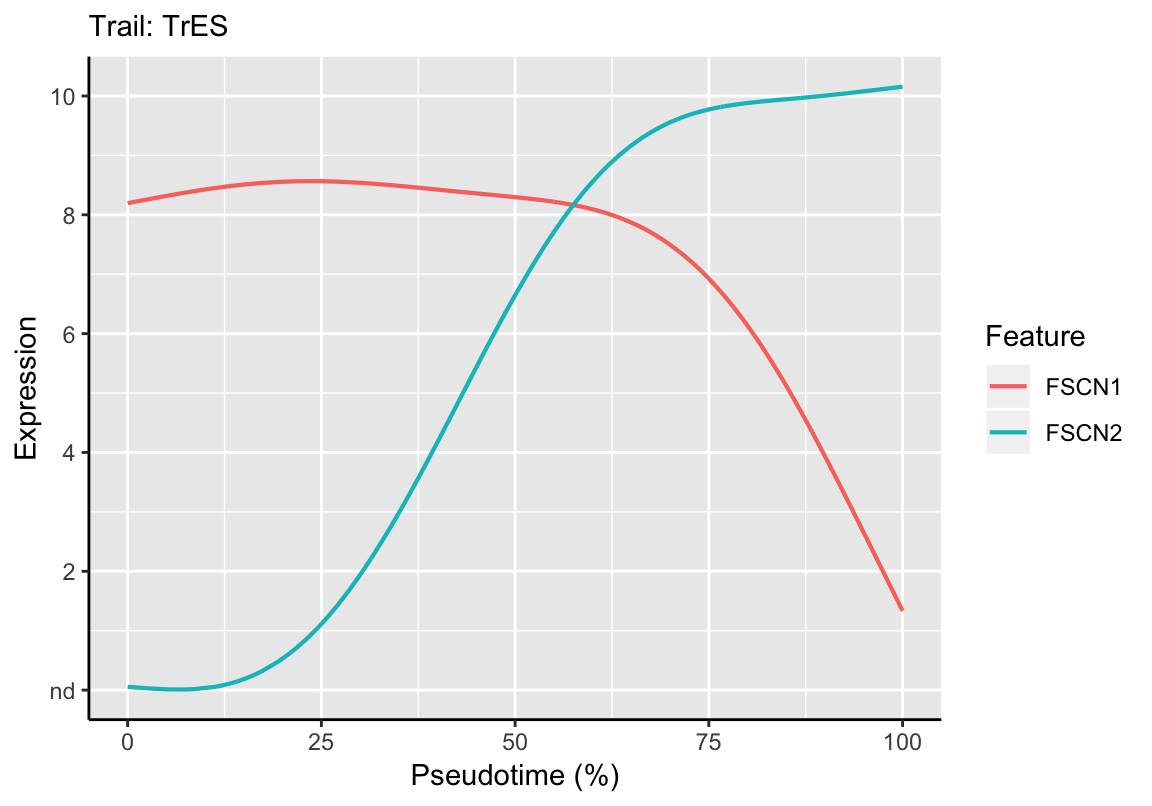
\includegraphics[width=0.7\linewidth]{CellTrails-handbook_files/figure-latex/unnamed-chunk-71-1}

By using the fitting function \texttt{fitDynamic}, the
similarity/correspondence between curves can be quantified. This allows
a quantitative assessment of the observed anticorrelation seen in the
plot above between \emph{FSCN1} and \emph{FSCN2}:

\begin{Shaded}
\begin{Highlighting}[]
\NormalTok{fscn1_fit <-}\StringTok{ }\KeywordTok{fitDynamic}\NormalTok{(exBundle, }\DataTypeTok{trail_name=}\StringTok{"TrES"}\NormalTok{, }\DataTypeTok{feature_name=}\StringTok{"FSCN1"}\NormalTok{)}
\NormalTok{fscn2_fit <-}\StringTok{ }\KeywordTok{fitDynamic}\NormalTok{(exBundle, }\DataTypeTok{trail_name=}\StringTok{"TrES"}\NormalTok{, }\DataTypeTok{feature_name=}\StringTok{"FSCN2"}\NormalTok{)}

\CommentTok{# Correlation}
\KeywordTok{cor}\NormalTok{(fscn1_fit}\OperatorTok{$}\NormalTok{expression, fscn2_fit}\OperatorTok{$}\NormalTok{expression)}
\end{Highlighting}
\end{Shaded}

\begin{verbatim}
## [1] -0.6432156
\end{verbatim}

\section{Dynamic Comparison: Between
Trails}\label{dynamic-comparison-between-trails}

Genes have non-uniform expression rates and each trail has a distinct
set of upregulated features, but also contains unequal numbers of
samples. Since pseudotime is computed based on expression differences
between individual samples, the pseudotime axis may be distorted,
leading to stretched or compressed sections of longitudinal expression
data that make comparisons of such trails challenging. To align
different trails, despite these differences, \emph{CellTrails} employs a
strategy that has long been known in speech recognition, called dynamic
time warping \citep{sakoe1978}. Feature expression dynamics are modeled
analogous to how dynamic time warping is used to align phonetic dynamics
present in speech. Innate non-linear variation in the length of
individual phonemes (i.e., states) is appropriately modeled, which
results in stretching and shrinking of word (i.e., trail) segments. This
allows the computation of inter-trail alignment warps of individual
expression time series that are similar but locally out of phase. The
overall dissimilarity between two expression time series can be
estimated by the root-mean-square deviation (\emph{RMSD}), the total
deviation (\emph{TD}), the area between curves (\emph{ABC}), or
Pearson's correlation coefficient (\emph{COR}) over all aligned
elements. The warp and the corresponding quantitative score can be
computed using the function \texttt{contrastTrailExpr}.

\begin{Shaded}
\begin{Highlighting}[]
\CommentTok{# Compare ATOH1 dynamic}
\CommentTok{# Root-mean-square deviation}
\KeywordTok{contrastTrailExpr}\NormalTok{(exBundle, }\DataTypeTok{feature_names=}\KeywordTok{c}\NormalTok{(}\StringTok{"ATOH1"}\NormalTok{), }
                  \DataTypeTok{trail_names=}\KeywordTok{c}\NormalTok{(}\StringTok{"TrS"}\NormalTok{, }\StringTok{"TrES"}\NormalTok{), }\DataTypeTok{score=}\StringTok{"RMSD"}\NormalTok{)}
\end{Highlighting}
\end{Shaded}

\begin{verbatim}
##     ATOH1 
## 0.0321192
\end{verbatim}

\begin{Shaded}
\begin{Highlighting}[]
\CommentTok{# Total deviation}
\KeywordTok{contrastTrailExpr}\NormalTok{(exBundle, }\DataTypeTok{feature_names=}\KeywordTok{c}\NormalTok{(}\StringTok{"ATOH1"}\NormalTok{), }
                  \DataTypeTok{trail_names=}\KeywordTok{c}\NormalTok{(}\StringTok{"TrS"}\NormalTok{, }\StringTok{"TrES"}\NormalTok{), }\DataTypeTok{score=}\StringTok{"TD"}\NormalTok{)}
\end{Highlighting}
\end{Shaded}

\begin{verbatim}
##    ATOH1 
## 6.364661
\end{verbatim}

\begin{Shaded}
\begin{Highlighting}[]
\CommentTok{# Area between curves}
\KeywordTok{contrastTrailExpr}\NormalTok{(exBundle, }\DataTypeTok{feature_names=}\KeywordTok{c}\NormalTok{(}\StringTok{"ATOH1"}\NormalTok{), }
                  \DataTypeTok{trail_names=}\KeywordTok{c}\NormalTok{(}\StringTok{"TrS"}\NormalTok{, }\StringTok{"TrES"}\NormalTok{), }\DataTypeTok{score=}\StringTok{"ABC"}\NormalTok{)}
\end{Highlighting}
\end{Shaded}

\begin{verbatim}
##      ATOH1 
## 0.02300188
\end{verbatim}

\begin{Shaded}
\begin{Highlighting}[]
\CommentTok{# Pearson's correlation coefficient}
\KeywordTok{contrastTrailExpr}\NormalTok{(exBundle, }\DataTypeTok{feature_names=}\KeywordTok{c}\NormalTok{(}\StringTok{"ATOH1"}\NormalTok{), }
                  \DataTypeTok{trail_names=}\KeywordTok{c}\NormalTok{(}\StringTok{"TrS"}\NormalTok{, }\StringTok{"TrES"}\NormalTok{), }\DataTypeTok{score=}\StringTok{"COR"}\NormalTok{)}
\end{Highlighting}
\end{Shaded}

\begin{verbatim}
##     ATOH1 
## 0.9999033
\end{verbatim}

In this example, \emph{ATOH1} is expected to have a highly similar
dynamic between both trails. Therefore, \emph{RMSD}, \emph{TD},
\emph{ABC} values should be low and \emph{COR} values high relative to
other assayed features.

To identify features that differ between two trails, we can compute the
divergence for all features and analyze the \emph{Z}-score distribution
as derived by \texttt{scale}:

\begin{Shaded}
\begin{Highlighting}[]
\CommentTok{# Compare TrS and TrES dynamics}
\CommentTok{# Root-mean-square deviation}
\NormalTok{all_rmsd <-}\StringTok{ }\KeywordTok{contrastTrailExpr}\NormalTok{(exBundle, }
                              \DataTypeTok{trail_names=}\KeywordTok{c}\NormalTok{(}\StringTok{"TrS"}\NormalTok{, }\StringTok{"TrES"}\NormalTok{), }\DataTypeTok{score=}\StringTok{"RMSD"}\NormalTok{)}

\CommentTok{# Identify highly differing features}
\NormalTok{all_rmsd <-}\StringTok{ }\NormalTok{all_rmsd[all_rmsd }\OperatorTok{>}\StringTok{ }\DecValTok{0}\NormalTok{]}
\NormalTok{zscores <-}\StringTok{ }\KeywordTok{scale}\NormalTok{(}\KeywordTok{log}\NormalTok{(all_rmsd))}
\KeywordTok{sort}\NormalTok{(all_rmsd[zscores }\OperatorTok{>}\StringTok{ }\FloatTok{1.65}\NormalTok{])}
\end{Highlighting}
\end{Shaded}

\begin{verbatim}
##     SYN3    AKAP5      OCM   SLC8A1   ATP2B2    MYO1H   CAB39L   MCOLN3 
## 1.494187 1.529849 1.601328 1.903307 1.953127 1.981343 2.304601 2.417525 
##  CHRNA10    MYO3A     CIB2    TNNC2    SKOR2   LOXHD1     TMC2 
## 2.637487 2.671320 2.790146 3.051273 3.717097 4.129766 4.799793
\end{verbatim}

\section{Parallelization}\label{parallelization}

In the case one wants to compare a large number of features (e.g.~from
an RNA-Seq experiment), the computation can be significantly sped up by
parallel computing. In this example, we use the package
\emph{\href{https://CRAN.R-project.org/package=doSNOW}{doSNOW}}, but any
other package may also be used for this purpose.

\begin{Shaded}
\begin{Highlighting}[]
\KeywordTok{library}\NormalTok{(doSNOW)}
\CommentTok{# Register parallel backend}
\NormalTok{cpu.cl <-}\StringTok{ }\KeywordTok{makeCluster}\NormalTok{(parallel}\OperatorTok{::}\KeywordTok{detectCores}\NormalTok{() }\OperatorTok{*}\StringTok{ }\DecValTok{2}\NormalTok{)}
\KeywordTok{registerDoSNOW}\NormalTok{(cpu.cl)}

\CommentTok{# Compute warps}
\NormalTok{fnames <-}\StringTok{ }\KeywordTok{featureNames}\NormalTok{(exBundle)}
\NormalTok{all_rmsd <-}\StringTok{ }\KeywordTok{foreach}\NormalTok{(}\DataTypeTok{i=}\KeywordTok{seq_along}\NormalTok{(fnames), }\DataTypeTok{.combine=}\NormalTok{rbind)  }\OperatorTok\StringTok{  }\NormalTok{\{}
\NormalTok{  g <-}\StringTok{ }\NormalTok{fnames[i]}
\NormalTok{  CellTrails}\OperatorTok{::}\KeywordTok{contrastTrailExpr}\NormalTok{(exBundle, }
                                \DataTypeTok{feature_name=}\NormalTok{g, }
                                \DataTypeTok{trail_names=}\KeywordTok{c}\NormalTok{(}\StringTok{"TrES"}\NormalTok{, }\StringTok{"TrS"}\NormalTok{), }
                                \DataTypeTok{score=}\StringTok{"RMSD"}\NormalTok{)}
\NormalTok{\}}
\KeywordTok{stopCluster}\NormalTok{(cpu.cl)}
\NormalTok{all_rmsd <-}\StringTok{ }\NormalTok{all_rmsd[, }\DecValTok{1}\NormalTok{]}
\KeywordTok{names}\NormalTok{(all_rmsd) <-}\StringTok{ }\NormalTok{fnames}
\end{Highlighting}
\end{Shaded}

\begin{Shaded}
\begin{Highlighting}[]
\CommentTok{# Identify highly differing features}
\NormalTok{all_rmsd <-}\StringTok{ }\NormalTok{all_rmsd[all_rmsd }\OperatorTok{>}\StringTok{ }\DecValTok{0}\NormalTok{]}
\NormalTok{zscores <-}\StringTok{ }\KeywordTok{scale}\NormalTok{(}\KeywordTok{log}\NormalTok{(all_rmsd))}
\KeywordTok{sort}\NormalTok{(all_rmsd[zscores }\OperatorTok{>}\StringTok{ }\FloatTok{1.65}\NormalTok{])}
\end{Highlighting}
\end{Shaded}

\begin{verbatim}
##     SYN3    AKAP5      OCM   SLC8A1   ATP2B2    MYO1H   CAB39L   MCOLN3 
## 1.494187 1.529849 1.601328 1.903307 1.953127 1.981343 2.304601 2.417525 
##  CHRNA10    MYO3A     CIB2    TNNC2    SKOR2   LOXHD1     TMC2 
## 2.637487 2.671320 2.790146 3.051273 3.717097 4.129766 4.799793
\end{verbatim}

\emph{Please note} that the advantage in computation time increases with
the number of features; for a small number of features parallel
computing may be slower than the sequential approach due to its
overhead.

\chapter{Appendix}\label{appendix}

\section{Protocols}\label{protocols}

The following protocols describe how this package can be used to perform
the data analysis shown in the original \emph{CellTrails} article.

\subsection{Chicken E15 Utricle Data}\label{chicken-e15-utricle-data}

\begin{Shaded}
\begin{Highlighting}[]
\CommentTok{# Load expression data}
\NormalTok{bundle <-}\StringTok{ }\KeywordTok{readRDS}\NormalTok{(}\KeywordTok{system.file}\NormalTok{(}\StringTok{"exdata"}\NormalTok{, }\StringTok{"bundle.rds"}\NormalTok{, }\DataTypeTok{package=}\StringTok{"CellTrails"}\NormalTok{))}

\CommentTok{# Manifold Learning}
\NormalTok{se <-}\StringTok{ }\KeywordTok{embedSamples}\NormalTok{(bundle)}
\NormalTok{d <-}\StringTok{ }\KeywordTok{findSpectrum}\NormalTok{(se}\OperatorTok{$}\NormalTok{eigenvalues, }\DataTypeTok{frac=}\DecValTok{100}\NormalTok{) }\CommentTok{#Similar to Figure 1E}
\KeywordTok{latentSpace}\NormalTok{(bundle) <-}\StringTok{ }\NormalTok{se}\OperatorTok{$}\NormalTok{components[, d]}

\CommentTok{# Clustering}
\KeywordTok{states}\NormalTok{(bundle) <-}\StringTok{ }\KeywordTok{findStates}\NormalTok{(bundle, }\DataTypeTok{min_size=}\FloatTok{0.01}\NormalTok{, }
                             \DataTypeTok{min_feat=}\DecValTok{5}\NormalTok{, }\DataTypeTok{max_pval=}\FloatTok{1e-04}\NormalTok{, }\DataTypeTok{min_fc=}\DecValTok{2}\NormalTok{)}

\CommentTok{# Sample Ordering}
\NormalTok{bundle <-}\StringTok{ }\KeywordTok{connectStates}\NormalTok{(bundle, }\DataTypeTok{l=}\DecValTok{10}\NormalTok{)}
\KeywordTok{showTrajInfo}\NormalTok{(bundle)}

\NormalTok{bundle <-}\StringTok{ }\KeywordTok{selectTrajectory}\NormalTok{(bundle, }\DataTypeTok{component=}\DecValTok{1}\NormalTok{)}
\NormalTok{bundle <-}\StringTok{ }\KeywordTok{fitTrajectory}\NormalTok{(bundle)}

\CommentTok{# CellTrails maps}
\CommentTok{# Please note: For illustration purposes, the layout was }
\CommentTok{# computed in yEd using functions write.ygraphml and }
\CommentTok{# read.ygraphml, and is part of the CellTrails package}
\NormalTok{tl <-}\StringTok{ }\KeywordTok{read.ygraphml}\NormalTok{(}\KeywordTok{system.file}\NormalTok{(}\StringTok{"exdata"}\NormalTok{, }\StringTok{"bundle.graphml"}\NormalTok{, }
                                \DataTypeTok{package=}\StringTok{"CellTrails"}\NormalTok{))}
\KeywordTok{trajLayout}\NormalTok{(bundle, }\DataTypeTok{adjust=}\OtherTok{TRUE}\NormalTok{) <-}\StringTok{ }\NormalTok{tl}

\CommentTok{# Define subtrail by adding a user-defined landmark}
\KeywordTok{userLandmarks}\NormalTok{(bundle) <-}\StringTok{ "Cell-8-57"}

\CommentTok{# Analysis of Expression Dynamics}
\NormalTok{bundle <-}\StringTok{ }\KeywordTok{addTrail}\NormalTok{(bundle, }\DataTypeTok{from=}\StringTok{"B3"}\NormalTok{, }\DataTypeTok{to=}\StringTok{"H9"}\NormalTok{, }\DataTypeTok{name=}\StringTok{"TrS"}\NormalTok{)}
\NormalTok{bundle <-}\StringTok{ }\KeywordTok{addTrail}\NormalTok{(bundle, }\DataTypeTok{from=}\StringTok{"B3"}\NormalTok{, }\DataTypeTok{to=}\StringTok{"H1"}\NormalTok{, }\DataTypeTok{name=}\StringTok{"TrES"}\NormalTok{)}
\NormalTok{bundle <-}\StringTok{ }\KeywordTok{addTrail}\NormalTok{(bundle, }\DataTypeTok{from=}\StringTok{"B3"}\NormalTok{, }\DataTypeTok{to=}\StringTok{"U1"}\NormalTok{, }\DataTypeTok{name=}\StringTok{"TrES*"}\NormalTok{)}

\CommentTok{# Inter-trail comparison (similar to Figure 5B)}
\NormalTok{rmsd_all <-}\StringTok{ }\KeywordTok{contrastTrailExpr}\NormalTok{(bundle, }\DataTypeTok{trail_names=}\KeywordTok{c}\NormalTok{(}\StringTok{"TrS"}\NormalTok{, }\StringTok{"TrES"}\NormalTok{))}
\NormalTok{rmsd_all <-}\StringTok{ }\NormalTok{rmsd_all[rmsd_all }\OperatorTok{>}\StringTok{ }\DecValTok{0}\NormalTok{]}
\KeywordTok{sort}\NormalTok{(rmsd_all[}\KeywordTok{scale}\NormalTok{(}\KeywordTok{log}\NormalTok{(rmsd_all)) }\OperatorTok{>}\StringTok{ }\FloatTok{1.65}\NormalTok{])}

\CommentTok{# -------------------------------}
\CommentTok{# Visualizations}
\CommentTok{# -------------------------------}
\CommentTok{# Plot size of clusters (similar to Figure 2E)}
\KeywordTok{plotStateSize}\NormalTok{(bundle)}

\CommentTok{# Plot expression distribution}
\KeywordTok{plotStateExpression}\NormalTok{(bundle, }\DataTypeTok{feature_name=}\StringTok{"OTOA"}\NormalTok{)}
\KeywordTok{plotStateExpression}\NormalTok{(bundle, }\DataTypeTok{feature_name=}\StringTok{"ATOH1"}\NormalTok{)}
\KeywordTok{plotStateExpression}\NormalTok{(bundle, }\DataTypeTok{feature_name=}\StringTok{"CALB2"}\NormalTok{)}
\KeywordTok{plotStateExpression}\NormalTok{(bundle, }\DataTypeTok{feature_name=}\StringTok{"ATP2B2"}\NormalTok{)}

\CommentTok{# Plot manifold (similar to Figure S4F)}
\KeywordTok{set.seed}\NormalTok{(}\DecValTok{1101}\NormalTok{)}
\NormalTok{gp <-}\StringTok{ }\KeywordTok{plotManifold}\NormalTok{(bundle, }\DataTypeTok{color_by=}\StringTok{"phenoName"}\NormalTok{, }\DataTypeTok{name=}\StringTok{"state"}\NormalTok{)}
\KeywordTok{manifold2D}\NormalTok{(bundle) <-}\StringTok{ }\NormalTok{gp}
\KeywordTok{plotManifold}\NormalTok{(bundle, }\DataTypeTok{color_by=}\StringTok{"phenoName"}\NormalTok{, }\DataTypeTok{name=}\StringTok{"fm143"}\NormalTok{)}
\KeywordTok{plotManifold}\NormalTok{(bundle, }\DataTypeTok{color_by=}\StringTok{"featureName"}\NormalTok{, }\DataTypeTok{name=}\StringTok{"OTOA"}\NormalTok{)}
\KeywordTok{plotManifold}\NormalTok{(bundle, }\DataTypeTok{color_by=}\StringTok{"featureName"}\NormalTok{, }\DataTypeTok{name=}\StringTok{"CALB2"}\NormalTok{)}

\CommentTok{# Plot state trajectory graph (similar to Figure 1G)}
\KeywordTok{plotStateTrajectory}\NormalTok{(bundle, }\DataTypeTok{color_by=}\StringTok{"phenoName"}\NormalTok{, }
                    \DataTypeTok{name=}\StringTok{"fm143"}\NormalTok{, }\DataTypeTok{point_size=}\FloatTok{1.5}\NormalTok{, }
                    \DataTypeTok{label_offset=}\DecValTok{4}\NormalTok{, }\DataTypeTok{component=}\DecValTok{1}\NormalTok{)}
\KeywordTok{plotStateTrajectory}\NormalTok{(bundle, }\DataTypeTok{color_by=}\StringTok{"phenoName"}\NormalTok{, }
                    \DataTypeTok{name=}\StringTok{"origin"}\NormalTok{, }\DataTypeTok{point_size=}\FloatTok{1.5}\NormalTok{, }
                    \DataTypeTok{label_offset=}\DecValTok{4}\NormalTok{, }\DataTypeTok{component=}\DecValTok{1}\NormalTok{)}
\KeywordTok{plotStateTrajectory}\NormalTok{(bundle, }\DataTypeTok{color_by=}\StringTok{"featureName"}\NormalTok{, }
                    \DataTypeTok{name=}\StringTok{"OTOA"}\NormalTok{, }\DataTypeTok{point_size=}\DecValTok{5}\NormalTok{, }
                    \DataTypeTok{label_offset=}\DecValTok{4}\NormalTok{, }\DataTypeTok{component=}\DecValTok{1}\NormalTok{)}
\KeywordTok{plotStateTrajectory}\NormalTok{(bundle, }\DataTypeTok{color_by=}\StringTok{"featureName"}\NormalTok{, }
                    \DataTypeTok{name=}\StringTok{"ATOH1"}\NormalTok{, }\DataTypeTok{point_size=}\DecValTok{5}\NormalTok{, }
                    \DataTypeTok{label_offset=}\DecValTok{4}\NormalTok{, }\DataTypeTok{component=}\DecValTok{1}\NormalTok{)}
\KeywordTok{plotStateTrajectory}\NormalTok{(bundle, }\DataTypeTok{color_by=}\StringTok{"featureName"}\NormalTok{, }
                    \DataTypeTok{name=}\StringTok{"CALB2"}\NormalTok{, }\DataTypeTok{point_size=}\DecValTok{5}\NormalTok{, }
                    \DataTypeTok{label_offset=}\DecValTok{4}\NormalTok{, }\DataTypeTok{component=}\DecValTok{1}\NormalTok{)}

\CommentTok{# Plot trajectory fit (similar to Figure 2E)}
\KeywordTok{plotTrajectoryFit}\NormalTok{(bundle)}

\CommentTok{# Plot CellTrails maps (similar to Figure 3 and Table S2)}
\KeywordTok{plotMap}\NormalTok{(bundle, }\DataTypeTok{color_by=}\StringTok{"phenoName"}\NormalTok{, }\DataTypeTok{name=}\StringTok{"fm143"}\NormalTok{)}
\KeywordTok{plotMap}\NormalTok{(bundle, }\DataTypeTok{color_by=}\StringTok{"featureName"}\NormalTok{, }
        \DataTypeTok{name=}\StringTok{"ATOH1"}\NormalTok{, }\DataTypeTok{type=}\StringTok{"raw"}\NormalTok{)}
\KeywordTok{plotMap}\NormalTok{(bundle, }\DataTypeTok{color_by=}\StringTok{"featureName"}\NormalTok{, }
        \DataTypeTok{name=}\StringTok{"ATOH1"}\NormalTok{, }\DataTypeTok{type=}\StringTok{"surface.fit"}\NormalTok{)}
\KeywordTok{plotMap}\NormalTok{(bundle, }\DataTypeTok{color_by=}\StringTok{"featureName"}\NormalTok{, }
        \DataTypeTok{name=}\StringTok{"ATOH1"}\NormalTok{, }\DataTypeTok{type=}\StringTok{"surface.se"}\NormalTok{)}
\KeywordTok{plotMap}\NormalTok{(bundle, }\DataTypeTok{color_by=}\StringTok{"featureName"}\NormalTok{, }
        \DataTypeTok{name=}\StringTok{"ATOH1"}\NormalTok{, }\DataTypeTok{type=}\StringTok{"surface.fit"}\NormalTok{, }\DataTypeTok{samples_only=}\OtherTok{TRUE}\NormalTok{)}

\CommentTok{# Plot landmarks}
\KeywordTok{plotMap}\NormalTok{(bundle, }\DataTypeTok{color_by=}\StringTok{"phenoName"}\NormalTok{, }\DataTypeTok{name=}\StringTok{"landmark"}\NormalTok{)}

\CommentTok{# Plot trails (similar to Figure 4K)}
\KeywordTok{plotTrail}\NormalTok{(bundle, }\DataTypeTok{name=}\StringTok{"TrS"}\NormalTok{)}
\KeywordTok{plotTrail}\NormalTok{(bundle, }\DataTypeTok{name=}\StringTok{"TrES"}\NormalTok{)}
\KeywordTok{plotTrail}\NormalTok{(bundle, }\DataTypeTok{name=}\StringTok{"TrES*"}\NormalTok{)}

\CommentTok{# Plot single dynamics (similar to Figure 4B,G and Table S2)}
\KeywordTok{plotDynamic}\NormalTok{(bundle, }\DataTypeTok{feature_name=}\StringTok{"CALB2"}\NormalTok{, }\DataTypeTok{trail_name=}\StringTok{"TrES"}\NormalTok{)}
\KeywordTok{plotDynamic}\NormalTok{(bundle, }\DataTypeTok{feature_name=}\StringTok{"ATP2B2"}\NormalTok{, }\DataTypeTok{trail_name=}\StringTok{"TrES"}\NormalTok{)}

\CommentTok{# Compare dynamics (similar to Figure 6A)}
\KeywordTok{plotDynamic}\NormalTok{(bundle, }
            \DataTypeTok{feature_name=}\KeywordTok{c}\NormalTok{(}\StringTok{"TECTA"}\NormalTok{, }\StringTok{"OTOA"}\NormalTok{, }\StringTok{"ATOH1"}\NormalTok{, }\StringTok{"POU4F3"}\NormalTok{, }
                           \StringTok{"MYO7A"}\NormalTok{, }\StringTok{"CALB2"}\NormalTok{, }\StringTok{"SYN3"}\NormalTok{, }\StringTok{"SKOR2"}\NormalTok{,}
                           \StringTok{"ATP2B2"}\NormalTok{, }\StringTok{"LOXHD1"}\NormalTok{, }\StringTok{"MYO3A"}\NormalTok{, }\StringTok{"TMC2"}\NormalTok{, }
                           \StringTok{"TNNC2"}\NormalTok{), }\DataTypeTok{trail_name=}\StringTok{"TrES"}\NormalTok{)}

\KeywordTok{plotDynamic}\NormalTok{(bundle, }
            \DataTypeTok{feature_name=}\KeywordTok{c}\NormalTok{(}\StringTok{"TECTA"}\NormalTok{, }\StringTok{"OTOA"}\NormalTok{, }\StringTok{"ATOH1"}\NormalTok{, }\StringTok{"POU4F3"}\NormalTok{, }
                           \StringTok{"MYO7A"}\NormalTok{, }\StringTok{"CALB2"}\NormalTok{, }\StringTok{"SYN3"}\NormalTok{, }\StringTok{"SKOR2"}\NormalTok{,}
                           \StringTok{"ATP2B2"}\NormalTok{, }\StringTok{"LOXHD1"}\NormalTok{, }\StringTok{"MYO3A"}\NormalTok{, }\StringTok{"TMC2"}\NormalTok{, }
                           \StringTok{"TNNC2"}\NormalTok{), }\DataTypeTok{trail_name=}\StringTok{"TrS"}\NormalTok{)}
\end{Highlighting}
\end{Shaded}

\subsection{Mouse P1 Utricle Data}\label{mouse-p1-utricle-data}

In the following, we provide a protocol to analyze the
publicly-available dataset containing single-cell RNASeq measurements of
14,313 genes in 120 cells from P1 mouse utricles
(\href{https://www.ncbi.nlm.nih.gov/geo/}{\emph{GEO}} accession code:
GSE71982). Experimental metadata was generated during cell sorting (GFP
and tdTomato fluorescence indicating major cell types). The processed
data (\texttt{mmu\_p1\_utricle.rda}) can be downloaded as
\emph{\href{http://bioconductor.org/packages/SingleCellExperiment}{SingleCellExperiment}}
object from
\href{https://github.com/dcellwanger/CellTrails-handbook/raw/master/exdata/mmu_p1_utricle.rds}{here}.
The trajectory layout (\texttt{mmu\_p1\_utricle.graphml}) can be
downloaded from
\href{https://github.com/dcellwanger/CellTrails-handbook/raw/master/exdata/mmu_p1_utricle.graphml}{here}.

If you use this dataset for your research, please cite the original work
by \citet{burns2015}.

\begin{Shaded}
\begin{Highlighting}[]
\CommentTok{# Load expression data}
\NormalTok{p1utricle <-}\StringTok{ }\KeywordTok{readRDS}\NormalTok{(}\StringTok{"mmu_p1_utricle.rds"}\NormalTok{)}

\CommentTok{# Feature Selection}
\KeywordTok{trajFeatureNames}\NormalTok{(p1utricle) <-}\StringTok{ }\KeywordTok{filterTrajFeaturesByDL}\NormalTok{(p1utricle, }\DataTypeTok{threshold=}\DecValTok{2}\NormalTok{)}
\KeywordTok{trajFeatureNames}\NormalTok{(p1utricle) <-}\StringTok{ }\KeywordTok{filterTrajFeaturesByCOV}\NormalTok{(p1utricle, }\DataTypeTok{threshold=}\NormalTok{.}\DecValTok{5}\NormalTok{)}
\KeywordTok{trajFeatureNames}\NormalTok{(p1utricle) <-}\StringTok{ }\KeywordTok{filterTrajFeaturesByFF}\NormalTok{(p1utricle)}

\KeywordTok{showTrajInfo}\NormalTok{(p1utricle)}

\CommentTok{# Manifold Learning}
\NormalTok{se <-}\StringTok{ }\KeywordTok{embedSamples}\NormalTok{(p1utricle)}
\NormalTok{d <-}\StringTok{ }\KeywordTok{findSpectrum}\NormalTok{(se}\OperatorTok{$}\NormalTok{eigenvalues)}
\KeywordTok{latentSpace}\NormalTok{(p1utricle) <-}\StringTok{ }\NormalTok{se}\OperatorTok{$}\NormalTok{components[, d]}

\CommentTok{# Clustering (parameters account for low sample size)}
\KeywordTok{states}\NormalTok{(p1utricle) <-}\StringTok{ }\KeywordTok{findStates}\NormalTok{(p1utricle, }\DataTypeTok{max_pval=}\FloatTok{1e-3}\NormalTok{, }\DataTypeTok{min_feat=}\DecValTok{2}\NormalTok{)}

\CommentTok{# Sample Ordering}
\NormalTok{p1utricle <-}\StringTok{ }\KeywordTok{connectStates}\NormalTok{(p1utricle)}
\NormalTok{p1utricle <-}\StringTok{ }\KeywordTok{fitTrajectory}\NormalTok{(p1utricle)}
\KeywordTok{showTrajInfo}\NormalTok{(p1utricle)}

\CommentTok{# CellTrails maps}
\NormalTok{tl <-}\StringTok{ }\KeywordTok{read.ygraphml}\NormalTok{(}\StringTok{"mmu_p1_utricle.graphml"}\NormalTok{)}
\KeywordTok{trajLayout}\NormalTok{(p1utricle) <-}\StringTok{ }\NormalTok{tl}

\CommentTok{# Analysis of Expression Dynamics}
\NormalTok{p1utricle <-}\StringTok{ }\KeywordTok{addTrail}\NormalTok{(p1utricle, }\DataTypeTok{from=}\StringTok{"H1"}\NormalTok{, }\DataTypeTok{to=}\StringTok{"H3"}\NormalTok{, }\DataTypeTok{name=}\StringTok{"Tr1"}\NormalTok{)}
\NormalTok{p1utricle <-}\StringTok{ }\KeywordTok{addTrail}\NormalTok{(p1utricle, }\DataTypeTok{from=}\StringTok{"H1"}\NormalTok{, }\DataTypeTok{to=}\StringTok{"H2"}\NormalTok{, }\DataTypeTok{name=}\StringTok{"Tr2"}\NormalTok{)}

\CommentTok{# Inter-trail comparison}
\NormalTok{rmsd_all <-}\StringTok{ }\KeywordTok{contrastTrailExpr}\NormalTok{(p1utricle, }\DataTypeTok{trail_names=}\KeywordTok{c}\NormalTok{(}\StringTok{"Tr1"}\NormalTok{, }\StringTok{"Tr2"}\NormalTok{))}
\NormalTok{rmsd_all <-}\StringTok{ }\NormalTok{rmsd_all[rmsd_all }\OperatorTok{>}\StringTok{ }\DecValTok{0}\NormalTok{]}
\KeywordTok{sort}\NormalTok{(rmsd_all[}\KeywordTok{scale}\NormalTok{(}\KeywordTok{log}\NormalTok{(rmsd_all)) }\OperatorTok{>}\StringTok{ }\FloatTok{1.65}\NormalTok{])}

\CommentTok{# Alternative: using parallel computing using doSNOW}
\KeywordTok{library}\NormalTok{(doSNOW)}
\NormalTok{cpu.cl <-}\StringTok{ }\KeywordTok{makeCluster}\NormalTok{(parallel}\OperatorTok{::}\KeywordTok{detectCores}\NormalTok{() }\OperatorTok{*}\StringTok{ }\DecValTok{2}\NormalTok{)}
\KeywordTok{registerDoSNOW}\NormalTok{(cpu.cl)}

\NormalTok{fnames <-}\StringTok{ }\KeywordTok{featureNames}\NormalTok{(p1utricle)}
\NormalTok{all_rmsd <-}\StringTok{ }\KeywordTok{foreach}\NormalTok{(}\DataTypeTok{i=}\KeywordTok{seq_along}\NormalTok{(fnames), }\DataTypeTok{.combine=}\NormalTok{rbind)  }\OperatorTok\StringTok{  }\NormalTok{\{}
\NormalTok{  g <-}\StringTok{ }\NormalTok{fnames[i]}
\NormalTok{  CellTrails}\OperatorTok{::}\KeywordTok{contrastTrailExpr}\NormalTok{(p1utricle, }\DataTypeTok{feature_name=}\NormalTok{g, }
                                \DataTypeTok{trail_names=}\KeywordTok{c}\NormalTok{(}\StringTok{"Tr1"}\NormalTok{, }\StringTok{"Tr2"}\NormalTok{), }\DataTypeTok{score=}\StringTok{"RMSD"}\NormalTok{)}
\NormalTok{\}}
\KeywordTok{stopCluster}\NormalTok{(cpu.cl)}
\NormalTok{all_rmsd <-}\StringTok{ }\NormalTok{all_rmsd[, }\DecValTok{1}\NormalTok{]}
\KeywordTok{names}\NormalTok{(all_rmsd) <-}\StringTok{ }\NormalTok{fnames}
\NormalTok{all_rmsd <-}\StringTok{ }\NormalTok{all_rmsd[all_rmsd }\OperatorTok{>}\StringTok{ }\DecValTok{0}\NormalTok{]}
\NormalTok{zscores <-}\StringTok{ }\KeywordTok{scale}\NormalTok{(}\KeywordTok{log}\NormalTok{(all_rmsd))}
\KeywordTok{sort}\NormalTok{(all_rmsd[zscores }\OperatorTok{>}\StringTok{ }\FloatTok{1.65}\NormalTok{])}

\CommentTok{# -------------------------------}
\CommentTok{# Visualizations}
\CommentTok{# -------------------------------}
\CommentTok{# Plot size of clusters (similar to Figure 7A)}
\KeywordTok{plotStateSize}\NormalTok{(p1utricle)}

\CommentTok{# Plot expression distribution}
\KeywordTok{plotStateExpression}\NormalTok{(p1utricle, }\DataTypeTok{feature_name=}\StringTok{"Otoa"}\NormalTok{)}
\KeywordTok{plotStateExpression}\NormalTok{(p1utricle, }\DataTypeTok{feature_name=}\StringTok{"Atoh1"}\NormalTok{)}
\KeywordTok{plotStateExpression}\NormalTok{(p1utricle, }\DataTypeTok{feature_name=}\StringTok{"Sox2"}\NormalTok{)}

\CommentTok{# Plot manifold}
\KeywordTok{set.seed}\NormalTok{(}\DecValTok{1101}\NormalTok{)}
\NormalTok{gp <-}\StringTok{ }\KeywordTok{plotManifold}\NormalTok{(p1utricle, }\DataTypeTok{color_by=}\StringTok{"phenoName"}\NormalTok{, }\DataTypeTok{name=}\StringTok{"state"}\NormalTok{)}
\KeywordTok{manifold2D}\NormalTok{(p1utricle) <-}\StringTok{ }\NormalTok{gp}
\KeywordTok{plotManifold}\NormalTok{(p1utricle, }\DataTypeTok{color_by=}\StringTok{"phenoName"}\NormalTok{, }\DataTypeTok{name=}\StringTok{"gate"}\NormalTok{)}
\KeywordTok{plotManifold}\NormalTok{(p1utricle, }\DataTypeTok{color_by=}\StringTok{"featureName"}\NormalTok{, }\DataTypeTok{name=}\StringTok{"Otoa"}\NormalTok{)}
\KeywordTok{plotManifold}\NormalTok{(p1utricle, }\DataTypeTok{color_by=}\StringTok{"featureName"}\NormalTok{, }\DataTypeTok{name=}\StringTok{"Fscn2"}\NormalTok{)}

\CommentTok{# Plot state trajectory graph (similar to Figure 1G)}
\KeywordTok{plotStateTrajectory}\NormalTok{(p1utricle, }\DataTypeTok{color_by=}\StringTok{"phenoName"}\NormalTok{, }
                    \DataTypeTok{name=}\StringTok{"gate"}\NormalTok{, }\DataTypeTok{point_size=}\FloatTok{1.5}\NormalTok{, }
                    \DataTypeTok{label_offset=}\DecValTok{4}\NormalTok{, }\DataTypeTok{component=}\DecValTok{1}\NormalTok{)}
\KeywordTok{plotStateTrajectory}\NormalTok{(p1utricle, }\DataTypeTok{color_by=}\StringTok{"featureName"}\NormalTok{, }
                    \DataTypeTok{name=}\StringTok{"Otoa"}\NormalTok{, }\DataTypeTok{point_size=}\DecValTok{5}\NormalTok{, }
                    \DataTypeTok{label_offset=}\DecValTok{4}\NormalTok{, }\DataTypeTok{component=}\DecValTok{1}\NormalTok{)}

\CommentTok{# Plot trajectory fit (similar to Figure 7A)}
\KeywordTok{plotTrajectoryFit}\NormalTok{(p1utricle)}

\CommentTok{# Plot CellTrails maps (similar to Figure 7C-E)}
\KeywordTok{plotMap}\NormalTok{(p1utricle, }\DataTypeTok{color_by=}\StringTok{"phenoName"}\NormalTok{, }\DataTypeTok{name=}\StringTok{"gate"}\NormalTok{)}
\KeywordTok{plotMap}\NormalTok{(p1utricle, }\DataTypeTok{color_by=}\StringTok{"featureName"}\NormalTok{, }
        \DataTypeTok{name=}\StringTok{"Atoh1"}\NormalTok{, }\DataTypeTok{type=}\StringTok{"raw"}\NormalTok{)}
\KeywordTok{plotMap}\NormalTok{(p1utricle, }\DataTypeTok{color_by=}\StringTok{"featureName"}\NormalTok{, }
        \DataTypeTok{name=}\StringTok{"Atoh1"}\NormalTok{, }\DataTypeTok{type=}\StringTok{"surface.fit"}\NormalTok{)}
\KeywordTok{plotMap}\NormalTok{(p1utricle, }\DataTypeTok{color_by=}\StringTok{"featureName"}\NormalTok{, }
        \DataTypeTok{name=}\StringTok{"Atoh1"}\NormalTok{, }\DataTypeTok{type=}\StringTok{"surface.se"}\NormalTok{)}
\KeywordTok{plotMap}\NormalTok{(p1utricle, }\DataTypeTok{color_by=}\StringTok{"featureName"}\NormalTok{, }
        \DataTypeTok{name=}\StringTok{"Atoh1"}\NormalTok{, }\DataTypeTok{type=}\StringTok{"surface.fit"}\NormalTok{, }
        \DataTypeTok{samples_only=}\OtherTok{TRUE}\NormalTok{)}

\CommentTok{# Plot landmarks}
\KeywordTok{plotMap}\NormalTok{(p1utricle, }\DataTypeTok{color_by=}\StringTok{"phenoName"}\NormalTok{, }\DataTypeTok{name=}\StringTok{"landmark"}\NormalTok{)}

\CommentTok{# Plot trails (similar to Figure 7F)}
\KeywordTok{plotTrail}\NormalTok{(p1utricle, }\DataTypeTok{name=}\StringTok{"Tr1"}\NormalTok{)}
\KeywordTok{plotTrail}\NormalTok{(p1utricle, }\DataTypeTok{name=}\StringTok{"Tr2"}\NormalTok{)}

\CommentTok{# Plot single dynamics (similar to Figure 7I)}
\KeywordTok{plotDynamic}\NormalTok{(p1utricle, }\DataTypeTok{feature_name=}\StringTok{"Fgf21"}\NormalTok{, }\DataTypeTok{trail_name=}\StringTok{"Tr2"}\NormalTok{)}
\KeywordTok{plotDynamic}\NormalTok{(p1utricle, }\DataTypeTok{feature_name=}\StringTok{"Fgf21"}\NormalTok{, }\DataTypeTok{trail_name=}\StringTok{"Tr1"}\NormalTok{)}

\CommentTok{# Compare dynamics}
\KeywordTok{plotDynamic}\NormalTok{(p1utricle, }\DataTypeTok{feature_name=}\KeywordTok{c}\NormalTok{(}\StringTok{"Fscn1"}\NormalTok{, }\StringTok{"Fscn2"}\NormalTok{), }\DataTypeTok{trail_name=}\StringTok{"Tr2"}\NormalTok{)}
\end{Highlighting}
\end{Shaded}

\section{Runtime}\label{runtime}

In this section, we illustrate that a \emph{CellTrails} analysis can be
performed in a reasonable period of time. The elapsed computational
runtime of each function was measured on a MacBook Pro (Early 2015) with
a 3.1 GHz Intel Core i7 processor, 16 GB 1867 MHz DDR3 RAM, and an Intel
Iris Graphics 6100 1536 MB graphics card.

\subsection{Protocol: Chicken E15 Utricle
Data}\label{protocol-chicken-e15-utricle-data}

This dataset consists of 183 features and 1,008 samples. The computation
time of the whole protocol as listed above took less then two minutes.
Let's assume that computing the layout takes about two minutes (starting
\emph{yEd}, running the layouter, saving the file), then the total
runtime is up to five minutes.

\subsection{Protocol: Mouse P1 Utricle
Data}\label{protocol-mouse-p1-utricle-data}

This dataset consists of 14,313 features and 120 samples. The
computation time of the whole protocol as listed above (with
parallelization of the inter-trail dynamics comparison) took less then
seven minutes. Let's assume that computing the layout takes about two
minutes (starting \emph{yEd}, running the layouter, saving the file),
then the total runtime is up to 10 minutes.

\section{Session Info}\label{session-info}

This manual was created with \emph{yEd} version 3.14.4.\\
The \emph{R} session and the system used to compile this document are
listed below.

\begin{Shaded}
\begin{Highlighting}[]
\KeywordTok{sessionInfo}\NormalTok{()}
\end{Highlighting}
\end{Shaded}

\begin{verbatim}
## R version 3.4.3 (2017-11-30)
## Platform: x86_64-apple-darwin15.6.0 (64-bit)
## Running under: macOS Sierra 10.12.4
## 
## Matrix products: default
## BLAS: /Library/Frameworks/R.framework/Versions/3.4/Resources/lib/libRblas.0.dylib
## LAPACK: /Library/Frameworks/R.framework/Versions/3.4/Resources/lib/libRlapack.dylib
## 
## locale:
## [1] en_US.UTF-8/en_US.UTF-8/en_US.UTF-8/C/en_US.UTF-8/en_US.UTF-8
## 
## attached base packages:
## [1] parallel  stats4    stats     graphics  grDevices utils     datasets 
## [8] methods   base     
## 
## other attached packages:
##  [1] CellTrails_0.99.12         SingleCellExperiment_1.0.0
##  [3] SummarizedExperiment_1.8.0 DelayedArray_0.4.1        
##  [5] matrixStats_0.52.2         Biobase_2.38.0            
##  [7] GenomicRanges_1.30.0       GenomeInfoDb_1.14.0       
##  [9] IRanges_2.12.0             S4Vectors_0.16.0          
## [11] BiocGenerics_0.24.0        BiocStyle_2.6.1           
## 
## loaded via a namespace (and not attached):
##   [1] backports_1.1.2         Hmisc_4.0-3            
##   [3] RcppEigen_0.3.3.3.1     plyr_1.8.4             
##   [5] igraph_1.1.2            lazyeval_0.2.1         
##   [7] sp_1.2-5                shinydashboard_0.6.1   
##   [9] splines_3.4.3           BiocParallel_1.12.0    
##  [11] ggplot2_2.2.1           scater_1.6.1           
##  [13] digest_0.6.12           htmltools_0.3.6        
##  [15] viridis_0.4.0           magrittr_1.5           
##  [17] checkmate_1.8.5         memoise_1.1.0          
##  [19] cluster_2.0.6           limma_3.34.3           
##  [21] xts_0.10-0              prettyunits_1.0.2      
##  [23] colorspace_1.3-2        blob_1.1.0             
##  [25] ggrepel_0.7.0           xfun_0.1               
##  [27] dplyr_0.7.4             RCurl_1.95-4.8         
##  [29] tximport_1.6.0          EnvStats_2.3.0         
##  [31] lme4_1.1-14             bindr_0.1              
##  [33] survival_2.41-3         zoo_1.8-0              
##  [35] glue_1.2.0              gtable_0.2.0           
##  [37] zlibbioc_1.24.0         XVector_0.18.0         
##  [39] MatrixModels_0.4-1      cba_0.2-19             
##  [41] car_2.1-6               kernlab_0.9-25         
##  [43] prabclus_2.2-6          DEoptimR_1.0-8         
##  [45] SparseM_1.77            VIM_4.7.0              
##  [47] scales_0.5.0            mvtnorm_1.0-6          
##  [49] DBI_0.7                 edgeR_3.20.1           
##  [51] Rcpp_0.12.14            dtw_1.18-1             
##  [53] laeken_0.4.6            viridisLite_0.2.0      
##  [55] xtable_1.8-2            progress_1.1.2         
##  [57] htmlTable_1.11.0        foreign_0.8-69         
##  [59] bit_1.1-12              proxy_0.4-20           
##  [61] mclust_5.4              Formula_1.2-2          
##  [63] DT_0.2                  vcd_1.4-4              
##  [65] htmlwidgets_0.9         FNN_1.1                
##  [67] RColorBrewer_1.1-2      fpc_2.1-10             
##  [69] acepack_1.4.1           modeltools_0.2-21      
##  [71] pkgconfig_2.0.1         XML_3.98-1.9           
##  [73] flexmix_2.3-14          nnet_7.3-12            
##  [75] locfit_1.5-9.1          dynamicTreeCut_1.63-1  
##  [77] labeling_0.3            rlang_0.1.4            
##  [79] reshape2_1.4.3          AnnotationDbi_1.40.0   
##  [81] munsell_0.4.3           tools_3.4.3            
##  [83] RSQLite_2.0             evaluate_0.10.1        
##  [85] stringr_1.2.0           maptree_1.4-7          
##  [87] yaml_2.1.16             knitr_1.20             
##  [89] bit64_0.9-7             robustbase_0.92-8      
##  [91] purrr_0.2.4             dendextend_1.6.0       
##  [93] bindrcpp_0.2            nlme_3.1-131           
##  [95] quantreg_5.34           whisker_0.3-2          
##  [97] mime_0.5                scran_1.6.6            
##  [99] biomaRt_2.34.0          pbkrtest_0.4-7         
## [101] compiler_3.4.3          rstudioapi_0.7         
## [103] curl_3.1                beeswarm_0.2.3         
## [105] e1071_1.6-8             smoother_1.1           
## [107] tibble_1.3.4            statmod_1.4.30         
## [109] stringi_1.1.6           lattice_0.20-35        
## [111] trimcluster_0.1-2       Matrix_1.2-12          
## [113] nloptr_1.0.4            lmtest_0.9-35          
## [115] data.table_1.10.4-3     bitops_1.0-6           
## [117] httpuv_1.3.5            R6_2.2.2               
## [119] latticeExtra_0.6-28     bookdown_0.7           
## [121] gridExtra_2.3           vipor_0.4.5            
## [123] boot_1.3-20             MASS_7.3-47            
## [125] assertthat_0.2.0        destiny_2.6.1          
## [127] rhdf5_2.22.0            rprojroot_1.2          
## [129] rjson_0.2.15            GenomeInfoDbData_0.99.1
## [131] diptest_0.75-7          mgcv_1.8-22            
## [133] grid_3.4.3              rpart_4.1-11           
## [135] minqa_1.2.4             tidyr_0.7.2            
## [137] class_7.3-14            rmarkdown_1.8          
## [139] Rtsne_0.13              TTR_0.23-2             
## [141] shiny_1.0.5             base64enc_0.1-3        
## [143] ggbeeswarm_0.6.0
\end{verbatim}

\bibliography{book.bib,articles.bib}


\end{document}
